\documentclass[12pt,a4paper]{article}

\usepackage[utf8]{inputenc}
\usepackage[T2A]{fontenc}
\usepackage[english,russian]{babel}
\usepackage{amsmath}
\usepackage{amssymb}
\usepackage{bm}
\usepackage{geometry}
\usepackage{hyperref}
\usepackage{graphicx}
\usepackage{setspace}
\usepackage{indentfirst}
\usepackage{enumitem}
\usepackage{float}
% Times New Roman font (Annex 7, §1.3 — TNR 12pt)
\usepackage{mathptmx}

\geometry{
  a4paper,
  left=25mm,
  right=10mm,
  top=20mm,
  bottom=20mm
}

% Annex 7, §1.3: line spacing 1.5, paragraph indent 1.25 cm
\onehalfspacing
\setlength{\parindent}{1.25cm}

% Annex 7, §1.4.1 & §1.4.2: figure captions below (centred) with en-dash;
% table captions above, left-aligned, with en-dash.
\usepackage{caption}
\usepackage{multirow}
\captionsetup[figure]{labelsep=endash}
\captionsetup[table]{singlelinecheck=false, justification=raggedright,
                     labelsep=endash, position=top}

\hypersetup{
  colorlinks=true,
  linkcolor=blue,
  urlcolor=blue,
  citecolor=blue
}
\urlstyle{rm}

\begin{document}

%----------------------------------------------------------------------
% Title page
%----------------------------------------------------------------------
\begin{titlepage}
  \begin{center}
    NATIONAL RESEARCH UNIVERSITY\\
    HIGHER SCHOOL OF ECONOMICS\\[1em]
    Faculty of Computer Science\\
    Bachelor's Programme ``Data Science And Business Analytics''\\[4em]

    Research Project Report on the Topic:\\[1em]
    Optimisation of Warehouse Slotting and Routing\\[5em]

    \begin{flushleft}
      Submitted by the Student:\\[0.5em]
      Korablina Maya Aleksandrovna\\
      group \#БПАД233, 3rd year of study\\[2em]

      Approved by the Project Supervisor:\\[0.5em]
      Korneluyk Egor\\
      Faculty of Computer Science, HSE University
    \end{flushleft}

    \vfill
    Moscow 2026
  \end{center}
\end{titlepage}

%----------------------------------------------------------------------
% Table of Contents
%----------------------------------------------------------------------
\tableofcontents
\newpage

%----------------------------------------------------------------------
\section*{Abstract}
\addcontentsline{toc}{section}{Abstract}
%----------------------------------------------------------------------

This paper studies warehouse order picking optimisation through the integration of
analytical inventory classification and spatial movement analysis. Traditional approaches
rely either on ABC$\times$XYZ analysis or on spatial tools such as RTLS tracking and
heat maps, but these methods are usually applied independently, which limits their
effectiveness.

The study proposes a unified framework that combines ABC$\times$XYZ analysis,
simulated RTLS data, heat-map-based congestion modelling, and routing algorithms
in a single graph-based model, where edge weights include both physical distance
and congestion penalties.

Computational experiments on synthetic warehouse data show that the proposed
method reduces both average route length and aisle congestion compared with
non-integrated approaches in the tested single-depot setting.

\bigskip

В работе изучается задача оптимизации комплектации заказов на складе через
интеграцию аналитической классификации запасов и пространственного анализа
перемещений. Традиционные подходы опираются либо на ABC$\times$XYZ-анализ, либо
на пространственные инструменты мониторинга (RTLS, тепловые карты), но обычно
применяются раздельно, что снижает их эффективность.

В работе предлагается единая модель, объединяющая ABC$\times$XYZ-анализ,
симулированные данные RTLS, построение тепловых карт и алгоритмы маршрутизации
в одном графовом представлении, где вес ребра зависит как от расстояния, так
и от загруженности.

Результаты вычислительных экспериментов на синтетических данных показывают,
что предложенный метод снижает как средний путь сборки, так и уровень
загруженности проходов по сравнению с неинтегрированными подходами в
исследованной конфигурации склада с одним пунктом приёма/выдачи.

%----------------------------------------------------------------------
\section*{Keywords}
\addcontentsline{toc}{section}{Keywords}
%----------------------------------------------------------------------

Warehouse optimisation; ABC$\times$XYZ analysis; slotting problem; congestion-aware
routing; RTLS simulation; heat map analysis; order picking; graph-based modelling.

\newpage
%----------------------------------------------------------------------
\section{Introduction}
%----------------------------------------------------------------------

Warehouse operations constitute a critical component of modern supply chains. Storage
organization, order picking, and internal transportation directly influence operational costs,
service levels, and overall logistics performance. In many distribution centers, order picking
accounts for a significant share of total warehouse operating costs, making it one of the
primary targets for optimisation.

Traditionally, warehouse management relies on analytical inventory classification methods
such as ABC and XYZ analysis. ABC analysis ranks items according to their economic
importance, typically based on turnover or contribution to revenue, while XYZ analysis groups
items by demand stability. The combined ABC$\times$XYZ framework enables structured
prioritisation of stock keeping units (SKUs) and supports inventory planning decisions.
However, these methods do not consider the spatial layout of the warehouse or the dynamic
movement of operators and equipment.

Supply chain disruptions~--- most visibly those triggered by the Covid-19 pandemic~---
have shifted the strategic focus of logistics from pure cost minimisation toward operational
resilience and flexibility, accelerating the adoption of data-driven decision support across
all supply chain tiers~\cite{ref9}. At the warehouse level, this pressure manifests as a
growing need to respond to volatile demand patterns while maintaining service levels,
making the integration of analytical and spatial tools more urgent than ever.

At the same time, advances in digital technologies have enabled the collection of detailed
spatial-temporal data through real-time location systems (RTLS) and indoor positioning
systems (IPS). These technologies allow warehouses to monitor movement patterns, identify
congestion zones, and construct activity heat maps. Spatial analysis provides insight into
operational bottlenecks and traffic intensity within aisles. Nevertheless, such tools are often
applied separately from analytical inventory models and mainly serve monitoring rather than
integrated optimisation purposes.

The separation between demand-based prioritisation and spatial congestion analysis limits
the effectiveness of warehouse optimisation strategies. Classical ABC$\times$XYZ slotting
improves placement decisions but ignores aisle load and traffic interactions. Conversely,
congestion-aware routing can reduce local bottlenecks but does not differentiate between
high- and low-priority SKUs. As a result, warehouse systems frequently optimize isolated
components rather than the entire process.

This study focuses on small-to-medium warehouses (approximately 1\,000--5\,000\,m$^2$,
500--5\,000~SKUs) that are common among regional third-party logistics (3PL) providers,
e-commerce fulfillment centres, wholesale distributors, and spare-parts depots. A key
characteristic of this segment is the \emph{single-depot} configuration: receiving and
dispatch share the same access point, and pickers follow a \emph{return-to-origin} route.
This configuration corresponds to the classical return routing problem studied since
Ratliff and Rosenthal~\cite{ref_ratliff} and further developed by
Petersen~\cite{ref_petersen}, as opposed to the dual-depot setups typical of
large-scale distribution centres with separate inbound and outbound docks.

Within this operational setting, the separation between demand-based and spatial
optimisation methods is particularly problematic. A single chokepoint near the depot
concentrates nearly all picker traffic, so even a well-classified inventory will generate
heavy congestion if spatial constraints are ignored. The present study addresses this
limitation by proposing an integrated framework that
simultaneously accounts for inventory importance, demand variability, and spatial congestion.
The warehouse is modelled as a graph, where nodes represent pick locations and
intersections, and edges represent feasible movements. Heat map data derived from simulated
RTLS tracks are incorporated into edge weights as congestion penalties. Slotting decisions
are informed by ABC$\times$XYZ classification, while routing is performed using
congestion-aware shortest-path algorithms.

The innovative contribution of this work lies in the explicit integration of analytical inventory
prioritisation with spatial-temporal congestion modelling within a single optimisation
framework. Unlike existing approaches that treat these components independently, the
proposed model evaluates their combined impact on operational performance.

\paragraph{Structure of the paper.}
The remainder of the report is organised as follows.
Section~2 reviews the relevant literature on inventory classification,
RTLS-based spatial tracking, slotting strategies, and order picking routing,
and positions the present work in this context.
Section~3 gives the conceptual overview of the proposed method.
Section~4 provides the formal problem formulation (sets, decision variables,
cost structure, and objective function).
Section~5 describes the experimental setup: the warehouse layout, the SKU
dataset, the ABC$\times$XYZ classification, the baseline graph model, and
the $2 \times 2$ experimental design with its four evaluation metrics.
Section~6 reports the results for Config~A (congestion-aware routing on
classical slotting), including a sensitivity analysis on the congestion
penalty~$\lambda$.
Section~7 reports the results for Config~B (heat-map-informed slotting
under shortest-path routing) and compares six concrete slotting strategies
(DWC, HZR, TAPS, Aisle-Balanced, AAHMS, and the exploratory CAS).
Section~8 reports Config~C, which closes the $2 \times 2$ design by
combining the two interventions, and reports the full $7 \times 2$ matrix
of slottings under both routing algorithms.
Section~9 concludes with the main findings and limitations,
and Section~10 outlines directions for future work.

%----------------------------------------------------------------------
\section{Overview of Bibliographical Sources}
%----------------------------------------------------------------------

The reviewed literature covers four major research directions relevant to warehouse
optimisation: inventory classification methods, RTLS-based spatial tracking, slotting
optimisation, and warehouse digitalisation.

Trubchenko et al.~\cite{ref1} apply ABC$\times$XYZ analysis to the inventory of
Karandash LLC, a Russian commercial enterprise with approximately 30\,000 office supply
SKUs. ABC analysis ranks items by annual sales volume, while XYZ quantifies demand
stability using the coefficient of variation $V = 100\sigma/\bar{q}$, with thresholds
X~$\leq$~10--15\%, Y~=~15--25\%, and Z~$>$~25\%. The study finds that all analysed
items fall into Group~Z, yielding three cross-groups~--- AZ, BZ, and~CZ~--- each with a
dedicated replenishment strategy. Applying these recommendations reduced inventory storage
costs by~20\%. Despite the practical impact, the method remains purely analytical:
it does not incorporate the spatial layout of the warehouse, movement patterns of operators,
or operational congestion effects, limiting its applicability to static inventory
planning scenarios.

Pekar\v{c}\'{i}kov\'{a} et al.~\cite{ref2} investigate simulation-based optimisation of
material supply using RTLS data in automotive production environments. Their work
integrates real-time tracking data with simulation models in order to analyze
spatial-temporal movement patterns, identify bottlenecks, and evaluate logistics routes.
While spatial dynamics are modelled in detail, the study does not include analytical inventory
prioritisation methods such as ABC$\times$XYZ classification. As a result, SKU-level
importance is not considered in routing or placement decisions.

Kofler et al.~\cite{ref3} explore affinity-based slotting strategies under dynamic order
patterns. Their research highlights the importance of grouping frequently co-ordered items
to reduce travel distances and improve picking efficiency. Although the approach incorporates
order structure and demand interdependencies, it does not integrate real-time congestion data
or spatial heat map analysis into routing decisions.

Winkelhaus and Grosse~\cite{ref4} present a systematic literature review of 114~articles
on Logistics~4.0, deriving a framework that links external triggers (mass customisation,
sustainability), digital technological building blocks (IoT, cyber-physical systems, Big
Data, cloud, mobile and AR-based systems) and logistics tasks across supply, intra-,
distribution and reverse domains. The review identifies warehousing and warehouse
management as the single most represented task in the sample, with IoT-based WMS and
real-time visibility repeatedly reported as drivers of improved order picking, inventory
accuracy and material handling. However, the authors explicitly note that the field
remains dominated by conceptual works and that the integration of analytical inventory
prioritisation with the spatial dynamics of intralogistics is still underexplored~--- the
exact gap addressed by the present work.

Stroumpoulis and Kopanaki~\cite{ref10} complement this picture at the strategic level.
Their systematic review of sustainable supply chain management under digital transformation
surveys how Big Data Analytics (BDA), IoT, and Blockchain technology (BT) are discussed
in the academic literature in relation to economic, social, and environmental sustainability.
The review reveals that these technologies are analysed almost exclusively through a
strategic or conceptual lens: researchers examine their role in supply chain design,
supplier selection, and triple-bottom-line reporting, but operational algorithmic frameworks
for applying BDA or IoT-derived data within intralogistics processes are largely absent.
This finding reinforces the gap identified by Winkelhaus and Grosse: while the potential
of digital technologies is extensively theorised at the macro level, their translation into
concrete routing and slotting optimisation algorithms remains an open research question
--- which the present work directly addresses.

The professional publication by LIDD Consultants~\cite{ref5} demonstrates the use of
warehouse productivity heat maps for visualizing traffic intensity and identifying high-load
zones. Heat maps provide valuable operational insights and support congestion analysis.
Nevertheless, the approach is primarily descriptive and is not formally integrated with
analytical SKU prioritisation or routing algorithms.

Overall, existing research addresses inventory prioritisation, spatial tracking, heat map
visualisation, and routing optimisation as largely independent problems. Analytical methods
such as ABC and XYZ classification provide demand-based prioritisation but lack spatial
awareness. Conversely, RTLS-based tracking and heat map analysis capture movement
dynamics but do not incorporate demand-driven importance of SKUs into decision-making
models.

The large-scale literature review by Casella et al.~\cite{ref7} (2023) provides direct academic
evidence that this separation is methodologically problematic. The study explicitly concludes
that order picking operations should be optimized through the joint solution of a wide
set of interdependent problems, and that sequential (isolated) optimisation of individual
design tasks is likely to yield suboptimal performance. This finding strongly supports
the integrated modelling approach adopted in the present work. Furthermore, Casella et al.
document that picker blocking and aisle congestion lead to increased idle time, waiting
periods, and overall efficiency losses --- providing academic justification for introducing the
congestion weight $c_e$ into the routing cost function $\mathrm{Cost}(e) = d_e + \lambda c_e$.

In the area of order picking routing, Ratliff and Rosenthal~\cite{ref_ratliff} (1983)
provide the foundational result for single-block warehouses with return-to-depot routing.
They prove that an optimal picking route in a rectangular warehouse with a single entry/exit
can be computed in polynomial time using dynamic programming. This result establishes the
theoretical basis for the routing setting adopted in the present study. Petersen~\cite{ref_petersen}
(1997) extends this line of work by comparing multiple routing heuristics in single-depot
warehouses and evaluating their performance under different order sizes and layout
configuration.

Practical industry evidence is provided by the GEODIS optimisation report~\cite{ref8}, which
documents a real-world warehouse transformation combining slotting reorganization and
wave-based routing improvement. The report directly confirms the hypothesis underlying the
present work: ``good slotting without good routing still leads to suboptimal results,
and good routing without good slotting means items are placed sub-optimally.''  The GEODIS
experience demonstrates that the true potential of warehouse optimisation lies in the
integration of intelligent slotting and routing strategies, since together they maximize
overall operational efficiency --- which is precisely the objective of the $2 \times 2$
experimental design proposed in this study.

The absence of a unified framework that integrates ABC$\times$XYZ analysis,
congestion-aware routing, and spatial heat map data represents the main research gap
addressed in this work. Although these approaches are widely used, they are usually applied
separately.

Inventory classification methods focus on demand characteristics and economic importance
of SKUs, but they do not consider warehouse layout or movement patterns. On the other
hand, RTLS-based tracking and heat maps analyze spatial activity and congestion, but they
do not include demand-based prioritisation. Routing models often minimise distance or time,
yet they typically ignore both SKU importance and dynamic congestion.

To the best of the author's knowledge, there is no clear methodological framework that
combines these three components within a single optimisation model. As highlighted in the
topic defence presentation, this separation limits the overall efficiency of warehouse
optimisation, since improving only one aspect does not guarantee improvement of the entire
system.

This study aims to address this gap by developing an integrated graph-based framework
that connects inventory prioritisation, congestion modelling, and routing decisions. The
proposed approach allows joint evaluation of slotting and routing strategies and supports
more comprehensive warehouse performance improvement.

%----------------------------------------------------------------------
\section{Overview of the Proposed Method}
%----------------------------------------------------------------------

This section presents the conceptual framework of the proposed approach to warehouse
slotting and routing optimisation. The method combines inventory classification, spatial
congestion modelling, and routing optimisation within a single integrated structure.

\subsection{General Concept}

The main objective of the proposed approach is to reduce both picking route length
and aisle congestion by jointly considering demand-based SKU prioritisation and
spatial warehouse activity. Route length is used as a proxy for picking time under
the standard assumption that movement speed is roughly constant.

Traditional warehouse optimisation methods usually focus on only one component of the
system. Inventory models prioritize items based on economic importance and demand
variability, while spatial tools analyze movement patterns and congestion. In contrast, the
proposed method connects these components and evaluates their interaction.

The framework is based on three main elements:
\begin{enumerate}
  \item ABC$\times$XYZ classification of SKUs,
  \item Heat map construction based on RTLS/IPS movement data (or simulated tracks),
  \item Congestion-aware routing within a graph-based warehouse model.
\end{enumerate}

These elements are not applied independently. Instead, they are integrated into a unified
decision-making model.

\subsection{Warehouse as a Graph}

The warehouse layout is represented as a graph $G = (V, E)$, where:
\begin{itemize}
  \item $V$ is the set of nodes representing aisle cells, intersections, and pick locations,
  \item $E$ is the set of edges representing feasible movements between nodes.
\end{itemize}

Each edge has a base distance that reflects physical movement cost. In addition, congestion
information derived from heat maps is associated with edges. This allows spatial activity to
influence routing decisions. Such representation enables consistent modelling of both slotting
and routing within the same structure.

\subsection{Slotting Logic}

At the first stage, SKUs are classified using ABC$\times$XYZ analysis. The ABC component
reflects economic importance, while the XYZ component captures demand stability.

High-priority items (for example, AX or AY groups) are placed in more accessible storage
locations. Lower-priority items (such as CZ group) are assigned to less accessible areas.

In the extended version of the method, congestion levels are also considered during slotting.
Storage locations are evaluated not only by their distance to the warehouse entrance, but
also by local traffic intensity. This allows better distribution of picking activity across the
warehouse.

\subsection{Routing Logic}

For each order, a picking route is constructed within the warehouse graph. The cost of
movement along an edge is defined as:
\[
  \mathrm{Cost} = \mathrm{Distance} + \lambda \cdot \mathrm{CongestionWeight},
\]
where $\lambda$ controls the influence of congestion on routing decisions.

If $\lambda = 0$, routing is based only on physical distance. If $\lambda > 0$, the model
prefers less congested paths, even if they are slightly longer.

This formulation allows flexible balance between shortest-path efficiency and congestion
avoidance.

\subsection{Experimental Design}

To evaluate the impact of different components, a $2 \times 2$ experimental design is used.

\noindent\textbf{Slotting strategies:}
\begin{itemize}
  \item ABC$\times$XYZ slotting,
  \item ABC$\times$XYZ + heat map slotting.
\end{itemize}

\noindent\textbf{Routing strategies:}
\begin{itemize}
  \item Shortest path routing,
  \item Congestion-aware routing.
\end{itemize}

This results in four configurations:
\begin{enumerate}
  \item ABC$\times$XYZ + shortest path,
  \item ABC$\times$XYZ + congestion-aware routing,
  \item ABC$\times$XYZ + heat map slotting + shortest path,
  \item ABC$\times$XYZ + heat map slotting + congestion-aware routing.
\end{enumerate}

Such structure makes it possible to evaluate separately the contribution of improved slotting
and congestion-aware routing, as well as their combined effect.

\subsection{Methodological Contribution}

The key contribution of the proposed approach lies in the integration of analytical inventory
prioritisation with spatial congestion modelling inside a unified graph-based framework.
Instead of optimizing isolated components, the method evaluates how demand structure and
movement dynamics influence each other.

This integrated perspective enables more comprehensive analysis of warehouse performance
and provides a foundation for further formal modelling and experimental evaluation.

%----------------------------------------------------------------------
\section{Formal Problem Formulation}
%----------------------------------------------------------------------

In this section, the warehouse slotting and routing problem is described in a formal way. The
goal is to define the main sets, decision variables, cost structure, and optimisation objective.

\subsection{Basic Sets}

Let:
\begin{itemize}
  \item $S = \{s_1, s_2, \ldots, s_n\}$ be the set of SKUs,
  \item $L = \{l_1, l_2, \ldots, l_m\}$ be the set of storage locations,
  \item $O = \{o_1, o_2, \ldots, o_K\}$ be the set of customer orders.
\end{itemize}

Each order $o_k \in O$ is a subset of SKUs:
\[
  o_k \subseteq S.
\]

Each SKU $s_i$ has a priority weight $w_i$ derived from the ABC$\times$XYZ classification.
Higher values of $w_i$ correspond to more important items.

\subsection{Warehouse Graph}

The warehouse layout is modelled as a graph:
\[
  G = (V, E),
\]
where:
\begin{itemize}
  \item $V$ is the set of nodes (aisle cells, intersections, pick positions),
  \item $E$ is the set of edges representing possible movements.
\end{itemize}

Each edge $e \in E$ has:
\begin{itemize}
  \item a base distance $d_e > 0$,
  \item a congestion weight $c_e \geq 0$ derived from heat map data.
\end{itemize}

\subsection{Slotting Decision}

The slotting problem consists of assigning each SKU to a storage location.
Define a binary decision variable:
\[
  x_{i,j} =
  \begin{cases}
    1, & \text{if SKU } s_i \text{ is assigned to location } l_j,\\
    0, & \text{otherwise.}
  \end{cases}
\]

Each SKU must be assigned to exactly one location:
\[
  \sum_{j=1}^{m} x_{i,j} = 1 \qquad \forall\, s_i \in S.
\]

Each storage location has limited capacity. For simplicity, assume capacity equal to 1:
\[
  \sum_{i=1}^{n} x_{i,j} \leq 1 \qquad \forall\, l_j \in L.
\]

\subsection{Routing Cost}

For each order $o_k$, a picking route is constructed in graph $G$.
The cost of traversing edge $e$ is defined as:
\[
  \mathrm{Cost}(e) = d_e + \lambda \cdot c_e,
\]
where $\lambda \geq 0$ controls the influence of congestion.

When $\lambda = 0$, routing depends only on physical distance. When $\lambda > 0$,
congestion avoidance becomes part of the routing decision.

Let $P_k$ denote the path chosen for order $o_k$. The total routing cost for this order is:
\[
  C_k = \sum_{e \in P_k} (d_e + \lambda \cdot c_e).
\]

This formulation corresponds to a variant of the return routing problem~\cite{ref_ratliff},
extended with congestion-aware edge weights controlled by $\lambda$.

\subsection{Objective Function}

The overall objective is to minimise the expected total picking cost over all orders.
Let $p_k$ denote the probability (or frequency) of order $o_k$. The objective function is:
\[
  \min \sum_{k=1}^{K} p_k \cdot C_k.
\]

Since routing depends on SKU locations, and SKU locations depend on slotting decisions
$x_{i,j}$, the routing cost is indirectly determined by slotting. Therefore, the problem
integrates:
\begin{itemize}
  \item slotting decisions $x_{i,j}$,
  \item congestion-aware routing,
  \item order demand structure.
\end{itemize}

\subsection{Integrated Nature of the Problem}

The complexity of the problem comes from the interaction between placement and routing.
Changing SKU locations modifies pick nodes in the graph, which changes optimal paths and
total cost.

The proposed framework does not aim to solve the global optimisation problem exactly.
Instead, it evaluates heuristic slotting and routing strategies within this formal structure and
compares their performance under different configurations.

%----------------------------------------------------------------------
\section{Experimental Setup}
%----------------------------------------------------------------------

This section describes the experimental environment used to evaluate the proposed slotting
and routing framework. The implementation is based on a simulated warehouse model
represented as a grid and a corresponding walkability graph.

\subsection{Warehouse Layout Generation}

The warehouse is modelled as a two-dimensional grid of size $R \times C$, which provides the
spatial structure for the graph $G = (V, E)$ defined in the previous section.

Each cell of the grid belongs to one of three categories:
\begin{itemize}
  \item $0$ --- aisle (walkable cell),
  \item $1$ --- storage location (shelf, non-walkable),
  \item $2$ --- door (walkable; used as both entrance and exit).
\end{itemize}

The set of storage locations $L = \{l_1, \ldots, l_m\}$ corresponds to all grid cells marked
as shelves (value 1). Each location $l_j \in L$ represents a potential assignment point for
SKU $s_i \in S$ through decision variable $x_{i,j}$ defined in the formal model.

For experimental simplicity, all storage locations are assumed to have identical capacity.
Each shelf cell can store at most one SKU unit, which corresponds to the capacity constraint
\[
  \sum_{i=1}^{n} x_{i,j} \leq 1, \qquad \forall\, l_j \in L.
\]

This assumption allows clear comparison of slotting strategies without introducing additional
variability related to heterogeneous storage capacity.

Shelves are arranged in parallel rows separated by aisles of fixed width. Each shelf block
has predefined dimensions (length and height), and shelf rows are separated by corridors to
allow movement of picking agents. This structured layout ensures that all pick locations are
accessible through walkable cells.

A single door is placed on the boundary of the grid and serves as both entry and exit point.
In the graph model, the door corresponds to a specific node $v_\mathrm{door} \in V$. All
picking routes start and end at this node, which allows consistent computation of routing
cost $C_k$ for each order $o_k \in O$.

The single-door configuration with a combined entry and exit reflects the operational
reality of small-to-medium warehouses, where receiving and dispatch typically share the
same access infrastructure due to space, security, or cost constraints. This is common
in regional 3PL facilities, e-commerce fulfillment centres, pharmaceutical and
controlled-access storage, cold-chain warehouses (where each additional door increases
heat loss), and buffer warehouses inside manufacturing plants. The resulting routing
problem --- where every picker starts at the depot, visits a set of shelf locations,
and returns to the same depot --- belongs to the return routing class formalised by
Ratliff and Rosenthal~\cite{ref_ratliff}.

With a grid resolution of approximately $1$~m per cell, the $52 \times 52$ grid
corresponds to a total floor area of roughly $2\,700$\,m$^2$, which is representative of
small-to-medium regional distribution facilities. The $|S| = 1\,000$ SKUs used in the
experiment fall within the typical range for this segment (1\,000--10\,000 SKUs).
The generated layout contains $|L| = 1\,040$ shelf cells, which is slightly larger
than $|S|$; the remaining $40$ shelf cells stay empty in every slotting
configuration, so the assignment $x_{i,j}$ is one-to-one on the placed SKUs.

The layout generation follows deterministic geometric rules to ensure:
\begin{itemize}
  \item Regular shelf alignment,
  \item Uniform aisle width,
  \item Full connectivity of walkable cells.
\end{itemize}

The generated layout features a uniform aisle structure without a dedicated front
cross-aisle near the depot. This design choice amplifies congestion concentration at the
entry point and may underestimate the effectiveness of routing-only interventions in
warehouses with more sophisticated aisle hierarchies (e.g., wide main aisles, front/back
cross-aisles, one-way picking lanes). Validation on layouts with heterogeneous aisle
widths is left for future work.

The resulting structure represents a simplified but realistic warehouse environment suitable
for controlled experimental comparison of slotting decisions $x_{i,j}$ and routing strategies.
In this model, each shelf cell represents a single pick location at the SKU level, abstracting
away physical bin sharing. Although real shelves in medium-sized warehouses often hold
5--20~SKUs per bin, the unit-capacity assumption isolates the spatial effect of slotting and
allows cleaner comparison between placement strategies.

\begin{figure}[h]
  \centering
  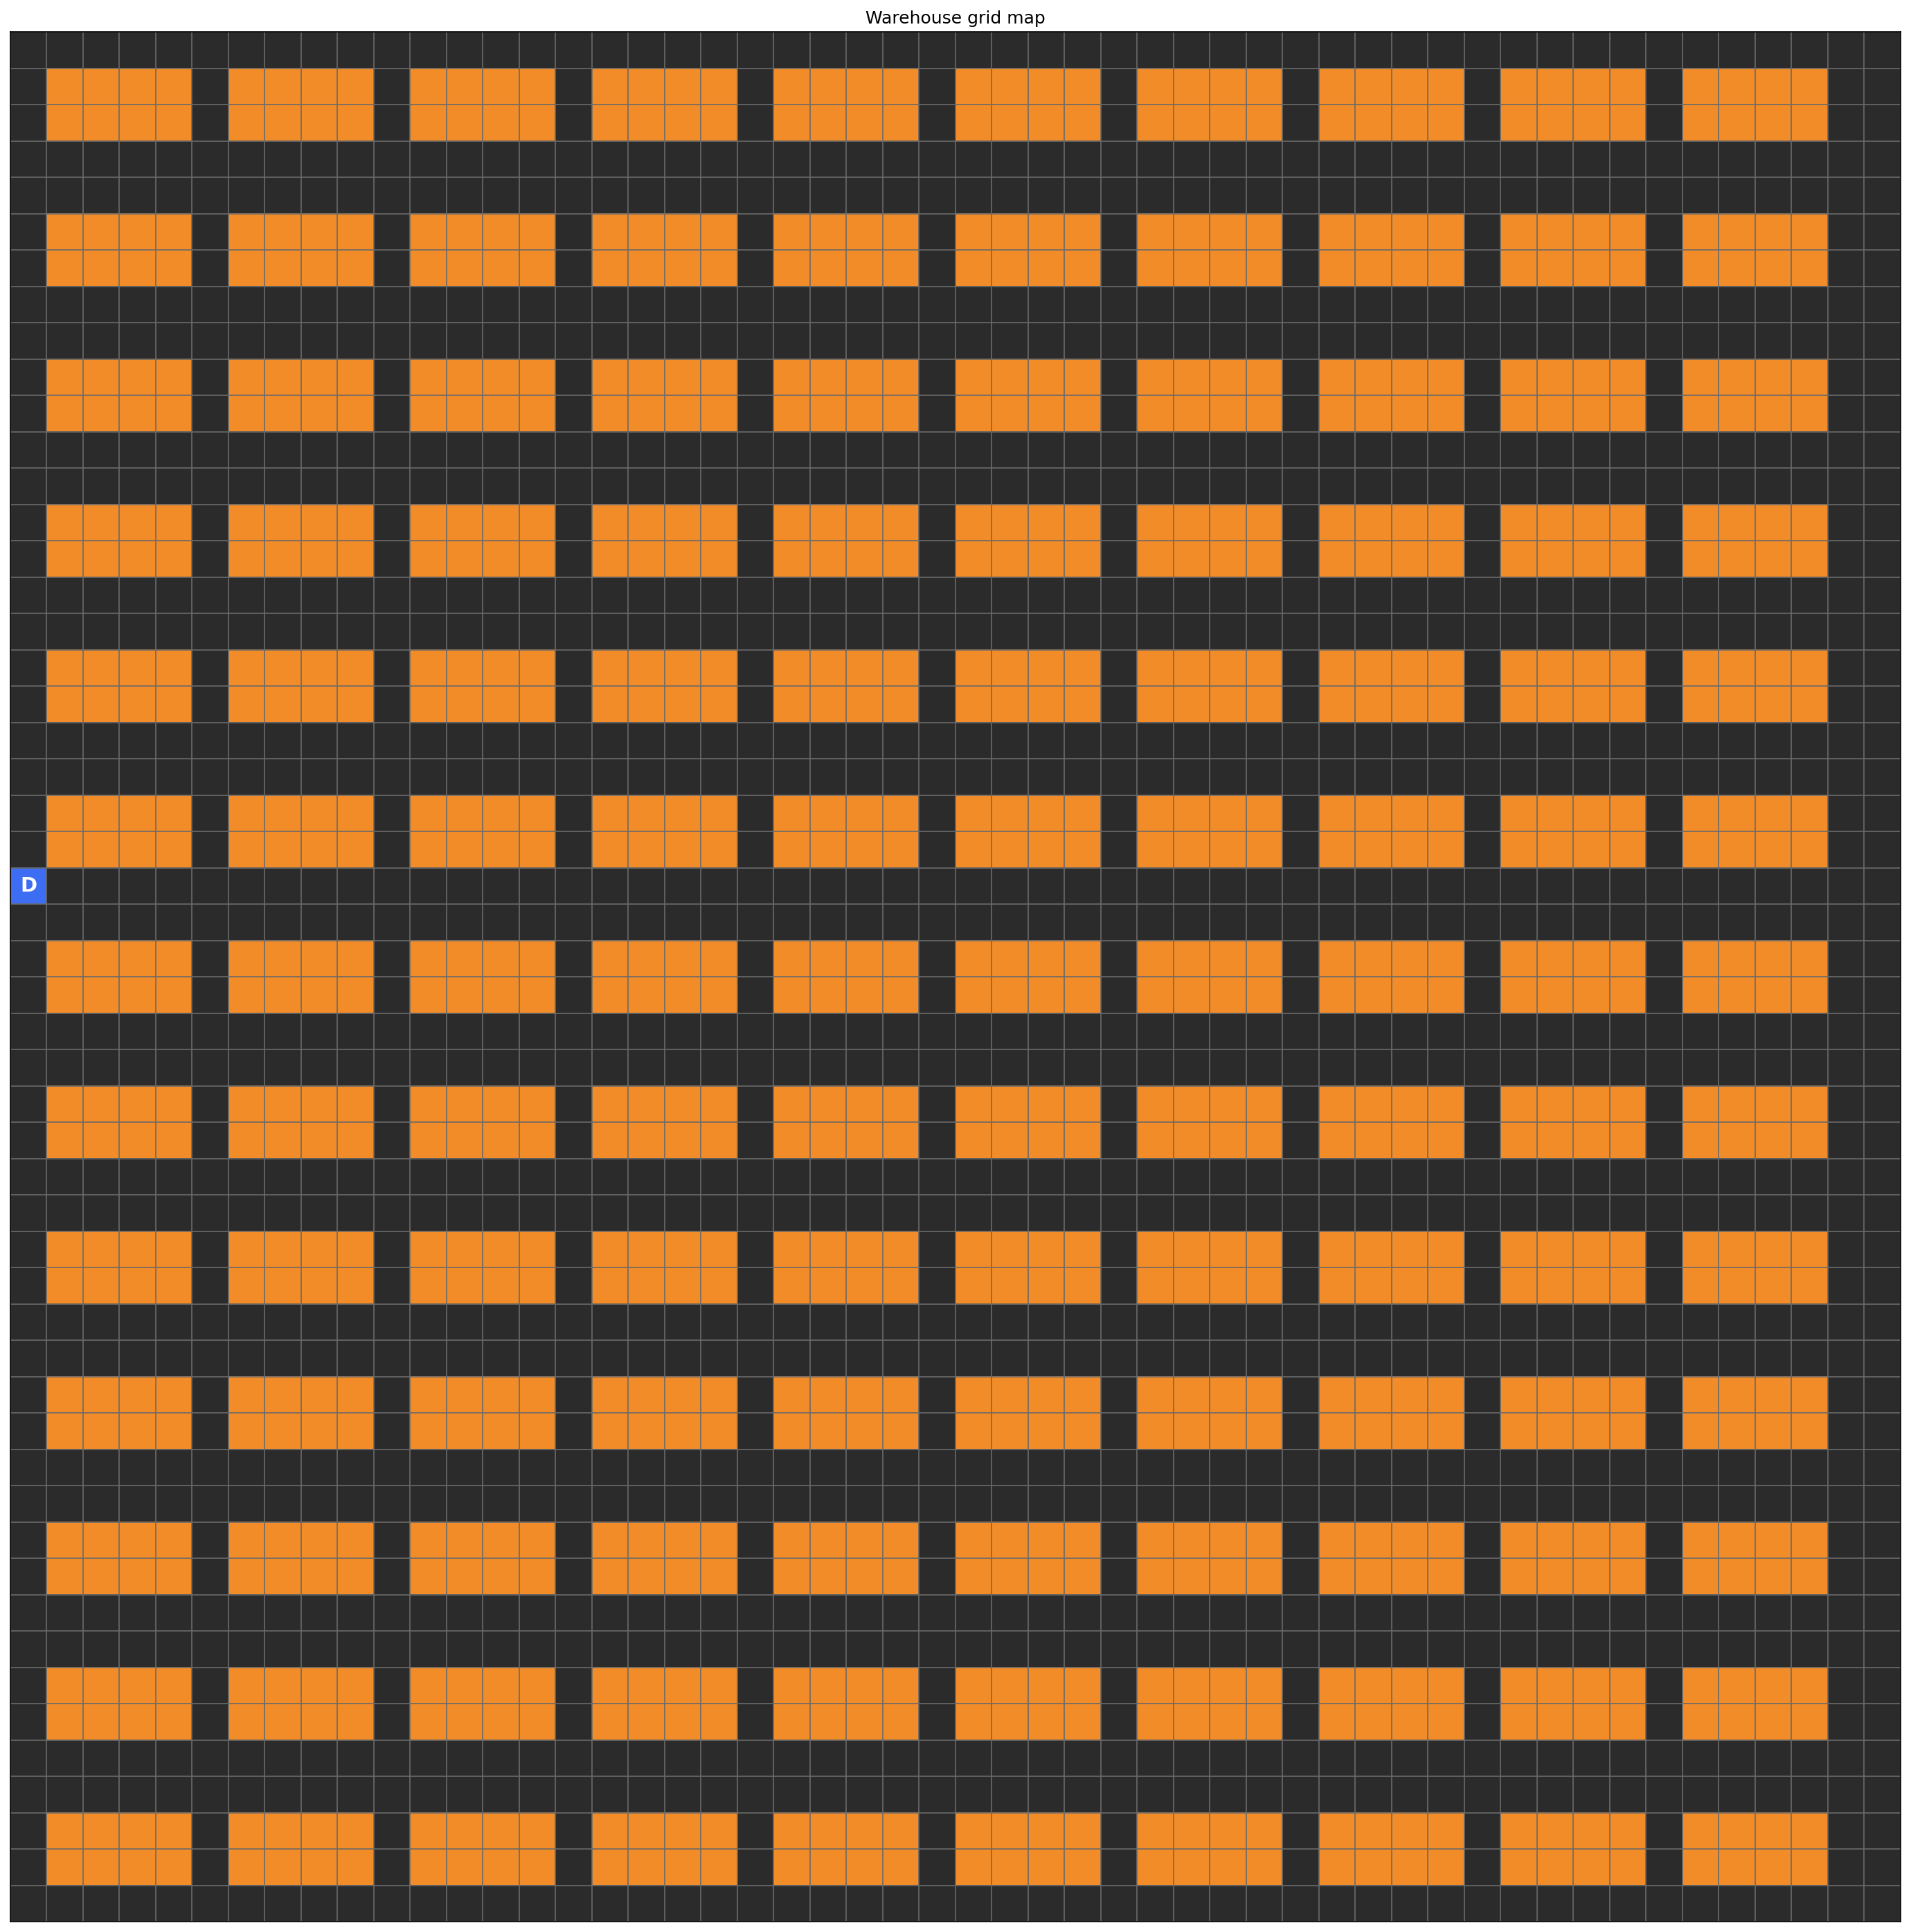
\includegraphics[width=0.8\textwidth]{warehouse_grid.png}
  \caption{Generated warehouse layout ($R \times C = 52 \times 52$). Dark cells
    represent walkable aisles, orange cells represent storage locations (shelves), and the
    blue cell on the left boundary at row~23 indicates the single door node $v_\mathrm{door}$.}
  \label{fig:layout}
\end{figure}

\subsection{Input SKU Dataset and ABC$\times$XYZ Classification}

The experiment uses a synthetic dataset consisting of $|S| = 1{,}000$ stock-keeping units
(SKUs) with 12~months of historical demand data (January through December). Each record
contains monthly demand figures, unit price, and total annual sales value. The dataset
was sourced from the publicly available ABC-XYZ Inventory Classification Dataset
published on Kaggle~\cite{ref6}.

This dataset was selected as the most suitable publicly available resource for
ABC$\times$XYZ inventory classification experiments. It provides exactly the data
structure required by the combined analysis methodology: item-level sales values for
ABC segmentation and monthly demand time series for XYZ variability assessment via the
coefficient of variation. Unlike generic sales datasets, it was specifically designed
to support supply chain segmentation tasks, making it directly applicable to the
warehouse slotting context studied in this work.

\paragraph{ABC Classification.}
Items are ranked by descending total annual units (demand volume) and segmented into three
groups following the APICS 70/20/10 convention by the number of items:
\begin{itemize}
  \item \textbf{A} --- top 20\,\% of items (200~SKUs) by annual demand volume ---
    the highest-priority group placed closest to the door;
  \item \textbf{B} --- next 30\,\% of items (300~SKUs) by annual demand volume;
  \item \textbf{C} --- remaining 50\,\% of items (500~SKUs) by annual demand volume.
\end{itemize}
Because order sampling is weighted by total annual units, the resulting order
probability distribution across classes is: A~--~56.2\,\%, B~--~33.7\,\%, C~--~10.1\,\%.
This distribution is substantially more balanced than the revenue-weighted alternative
(which concentrates 92.6\,\% of order probability in class~A), and reflects the reality
that items with high unit volume are not always the same as items with high revenue value.
In practice, item-count proportions frequently deviate from the 20/30/50 convention:
Trubchenko et al.~\cite{ref1} report a 5/16/79 distribution in a real retail assortment,
confirming that the thresholds define value boundaries, not item-count quotas.
The synthetic dataset used here adheres to the imposed convention by construction.

\paragraph{XYZ Classification.}
Demand stability is quantified by the coefficient of variation
$\mathrm{CV}_i = \sigma_i / \mu_i$,
where $\mu_i$ and $\sigma_i$ are the mean and standard deviation of monthly demand for
SKU~$s_i$. Items are classified using thresholds following Trubchenko et al.~\cite{ref1}:
\begin{itemize}
  \item \textbf{X} --- $\mathrm{CV}_i \leq 0.10$ (stable, predictable demand): 637~SKUs;
  \item \textbf{Y} --- $0.10 < \mathrm{CV}_i \leq 0.25$ (moderate variability): 216~SKUs;
  \item \textbf{Z} --- $\mathrm{CV}_i > 0.25$ (high variability, irregular demand): 147~SKUs.
\end{itemize}

The resulting $3 \times 3$ matrix of combined ABC$\times$XYZ categories is shown in
Figure~\ref{fig:abc_dist}. The mean coefficient of variation across all SKUs is
$\overline{\mathrm{CV}} = 0.143$, indicating that the dataset is predominantly
stable. X-type items account for 63.7\,\% of the total assortment, and the highest-priority
sub-class AX contains 136~SKUs --- these are positioned closest to the door in the
baseline slotting strategy. With demand-unit-based order sampling, the baseline traffic
Gini coefficient is $0.6697$ (compared to $0.8214$ under revenue-weighted sampling),
confirming that traffic is now more evenly spread across the warehouse.

\begin{figure}[h]
  \centering
  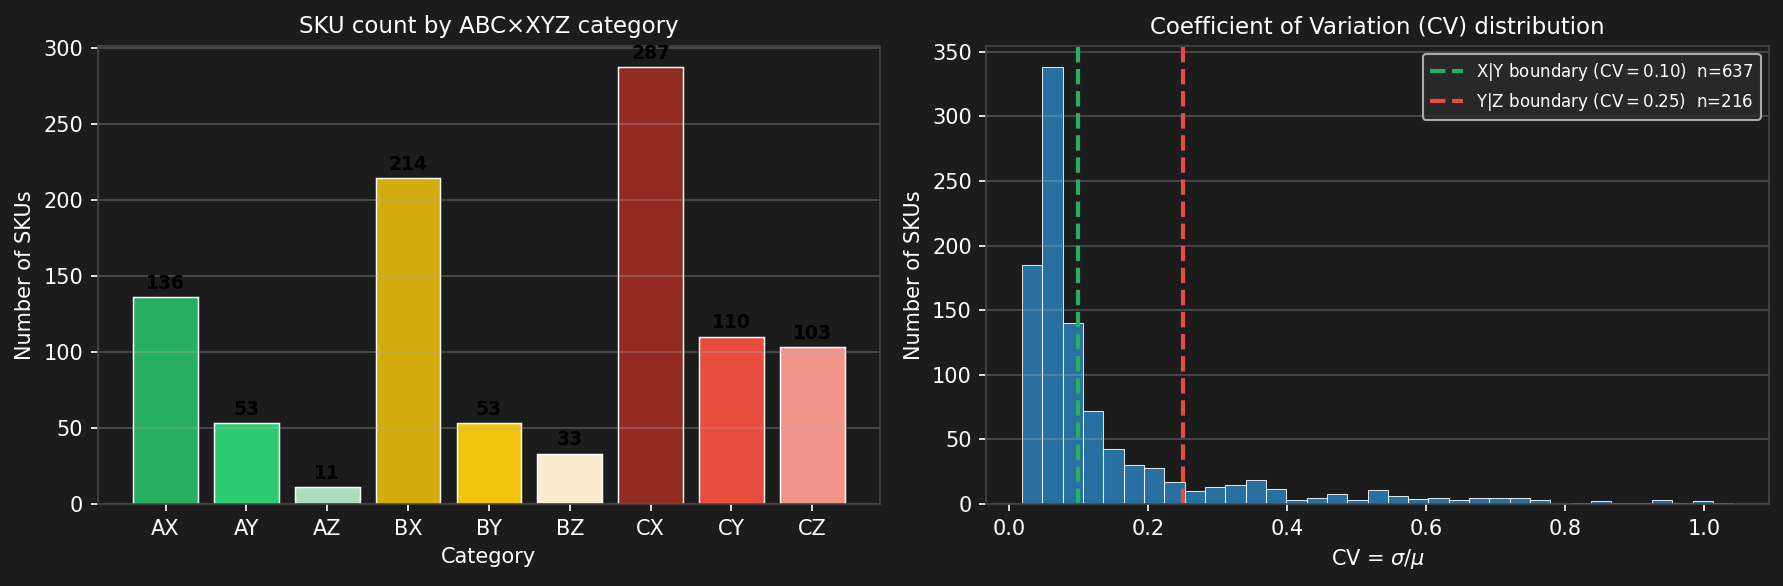
\includegraphics[width=\textwidth]{abc_distribution.png}
  \caption{Left: number of SKUs per ABC$\times$XYZ category. Right: distribution
    of the coefficient of variation $\mathrm{CV}$ with XYZ threshold boundaries
    ($\mathrm{CV} = 0.10$ and $\mathrm{CV} = 0.25$). X-type items dominate, reflecting
    stable seasonal demand patterns in the dataset.}
  \label{fig:abc_dist}
\end{figure}

\subsection{Baseline Graph Model and Initial Configurations}

After generating the grid, the warehouse is represented as a walkability graph
\[
  G = (V, E),
\]
as defined in Section~4.

The node set $V$ consists of all walkable grid cells (values 0 and 2), namely aisle cells and
the door. The edge set $E$ is defined using four-neighbor connectivity (up, down, left, right).
An edge $e = (u, v) \in E$ exists if both cells are walkable and adjacent.

In the baseline configuration, the movement cost between adjacent nodes is defined in the
simplest possible way. Each edge has unit weight:
\[
  d_e = 1.
\]

Thus, the distance between two nodes corresponds to the number of movement steps required
to travel between them. For any order $o_k \in O$, the routing cost under the baseline model
is computed as
\[
  C_k = \sum_{e \in P_k} d_e,
\]
where $P_k$ is the selected path in graph $G$. Since $d_e = 1$ for all edges, the total cost is
equal to the path length.

\subsubsection{Baseline A: Classical ABC$\times$XYZ Slotting}

In Baseline A, slotting decisions $x_{i,j}$ are determined solely by ABC$\times$XYZ
classification.

SKUs $s_i \in S$ are ranked according to their combined category (AX, AY, \ldots, CZ) and
economic importance. Storage locations $l_j \in L$ are ranked by their accessibility,
measured as the shortest-path distance from the door node $v_\mathrm{door}$ to the nearest
adjacent aisle cell.

Each SKU is assigned to exactly one shelf cell ($\sum_j x_{i,j} = 1$), and each shelf
cell holds at most one SKU ($\sum_i x_{i,j} \leq 1$). This corresponds to the
single-location assignment constraint from the formal model:
\[
  \sum_{j=1}^{m} x_{i,j} = 1,
  \qquad
  \sum_{i=1}^{n} x_{i,j} \leq 1.
\]

Importantly, congestion information is not used in this baseline. Placement decisions depend
only on demand priority and geometric accessibility.

Figure~\ref{fig:bfs_dist} shows the distribution of BFS distances across all
$|L| = 1{,}040$ shelf cells in the generated layout. The distribution is approximately
unimodal with a mean distance of $\overline{\delta} = 38.9$ steps. Shelf cells closest
to the door (distance $\leq 10$ steps) correspond to high-priority AX and AY zones;
cells at the far end of the range (distance $\geq 70$ steps) are assigned to CZ items.
The spread of the distribution reflects the geometric depth of the warehouse and confirms
that the slotting mechanism creates a meaningful priority gradient from door to rear.

\begin{figure}[h]
  \centering
  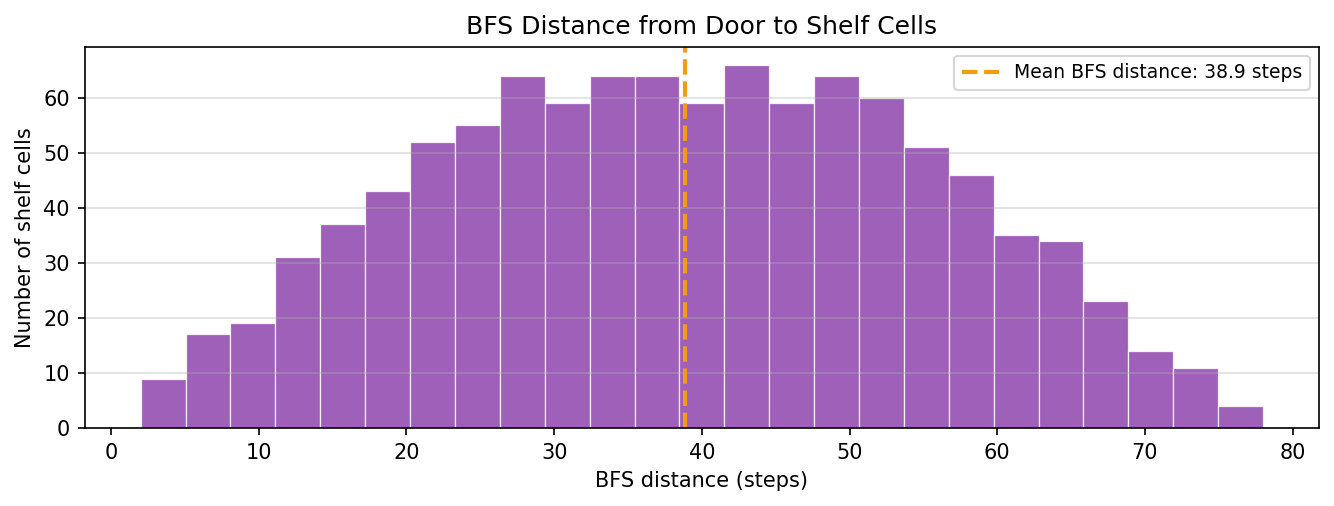
\includegraphics[width=0.85\textwidth]{bfs_distances.png}
  \caption{Distribution of BFS distances from the door node $v_\mathrm{door}$
    (row~23, left boundary) to all $|L| = 1{,}040$ shelf cells in the $52 \times 52$
    warehouse layout. The dashed line marks the mean distance $\overline{\delta} = 38.9$
    steps. AX-priority items occupy the left tail (shortest distances), while CZ items
    are assigned to the right tail (longest distances).}
  \label{fig:bfs_dist}
\end{figure}

\subsubsection{Baseline B: Distance-Based Routing Without Congestion}

Baseline B evaluates routing independently from congestion effects.

For each order $o_k \in O$, the picking path is constructed using a shortest-path search on
graph $G$ with edge weights $d_e = 1$. No congestion penalties $c_e$ are included in the
cost function. Therefore, routing decisions are based purely on geometric distance.

Slotting configuration remains the same as in Baseline A. The only difference is the routing
logic, which minimizes step count without considering traffic intensity.

\subsubsection{Order Generation and Connection to Baselines}

To evaluate Baseline A (slotting) and Baseline B (routing), a synthetic set of orders
\[
  O = \{o_1, o_2, \ldots, o_K\}
\]
is generated using demand information from the ABC$\times$XYZ dataset.

Let $d_i$ denote the average monthly demand of SKU $s_i \in S$. Each order is created by
sampling a fixed number of distinct SKUs without replacement. The probability of selecting
SKU $s_i$ is proportional to its average demand:
\[
  p_i = \frac{d_i}{\sum_{j=1}^{|S|} d_j}.
\]

This design reflects a realistic assumption: items with higher demand are more likely to
appear in customer orders. A fixed random seed is used to ensure reproducibility of the
generated orders.

The generated orders connect the two baselines in the following way:
\begin{itemize}
  \item Baseline A defines where each SKU is stored (the mapping from SKUs in $S$ to shelf
    locations in $L$).
  \item Baseline B defines how a picker moves through the warehouse graph $G = (V, E)$ to
    collect all SKUs from an order $o_k$.
\end{itemize}

For a given order $o_k$, the picker starts at the door node $v_\mathrm{door}$, visits the
locations needed for the SKUs in $o_k$, and returns to the door. The routing cost is computed
using the baseline edge weights $d_e = 1$, so the route cost is equal to the total number of
movement steps:
\[
  C_k = \sum_{e \in P_k} d_e.
\]

Since high-demand SKUs have larger probabilities $p_i$, they appear more often across
orders. As a result, the corresponding shelf areas are visited more frequently. Even without
explicit congestion modelling, this creates repeated traffic patterns near popular storage
zones, which motivates the later introduction of heat maps and congestion-aware routing.

\subsubsection{Order Picking Simulation in the Baseline Model}

To illustrate how the model operates in practice, we describe the processing of a single
order $o_k \in O$ under the baseline configuration.

\medskip
\noindent\textbf{Step 1: Identification of storage cells.}
Using the slotting configuration defined in Baseline A, each SKU from the order $o_k$ is
mapped to its assigned shelf cell(s) in the set $L$. Since shelf cells are non-walkable, the
picker cannot enter them directly.

\medskip
\noindent\textbf{Step 2: Selection of access points.}
For each required shelf cell, an adjacent walkable aisle cell is selected. Among the
neighboring aisle cells, the one with the smallest distance to the door $v_\mathrm{door}$ is
chosen. This ensures consistent distance-based accessibility evaluation.

\medskip
\noindent\textbf{Step 3: Route construction.}
The picker starts at the door node $v_\mathrm{door}$, sequentially visits all selected access
points, and finally returns to the door. The visiting order is determined by increasing
distance from the door, which corresponds to the baseline distance-based logic.

Each movement segment is computed using a shortest-path search on the graph $G = (V, E)$
with unit edge weights $d_e = 1$. Therefore, the total picking cost for order $o_k$ is equal
to the total number of movement steps:
\[
  C_k = \sum_{e \in P_k} d_e.
\]

\medskip
\noindent\textbf{Route Visualisation.}
Figure~\ref{fig:route} illustrates an example of a picking route under the baseline
configuration. The purple line represents the picker's movement through aisle cells,
and the numbered markers indicate the sequence of visited pick locations.

\begin{figure}[h]
  \centering
  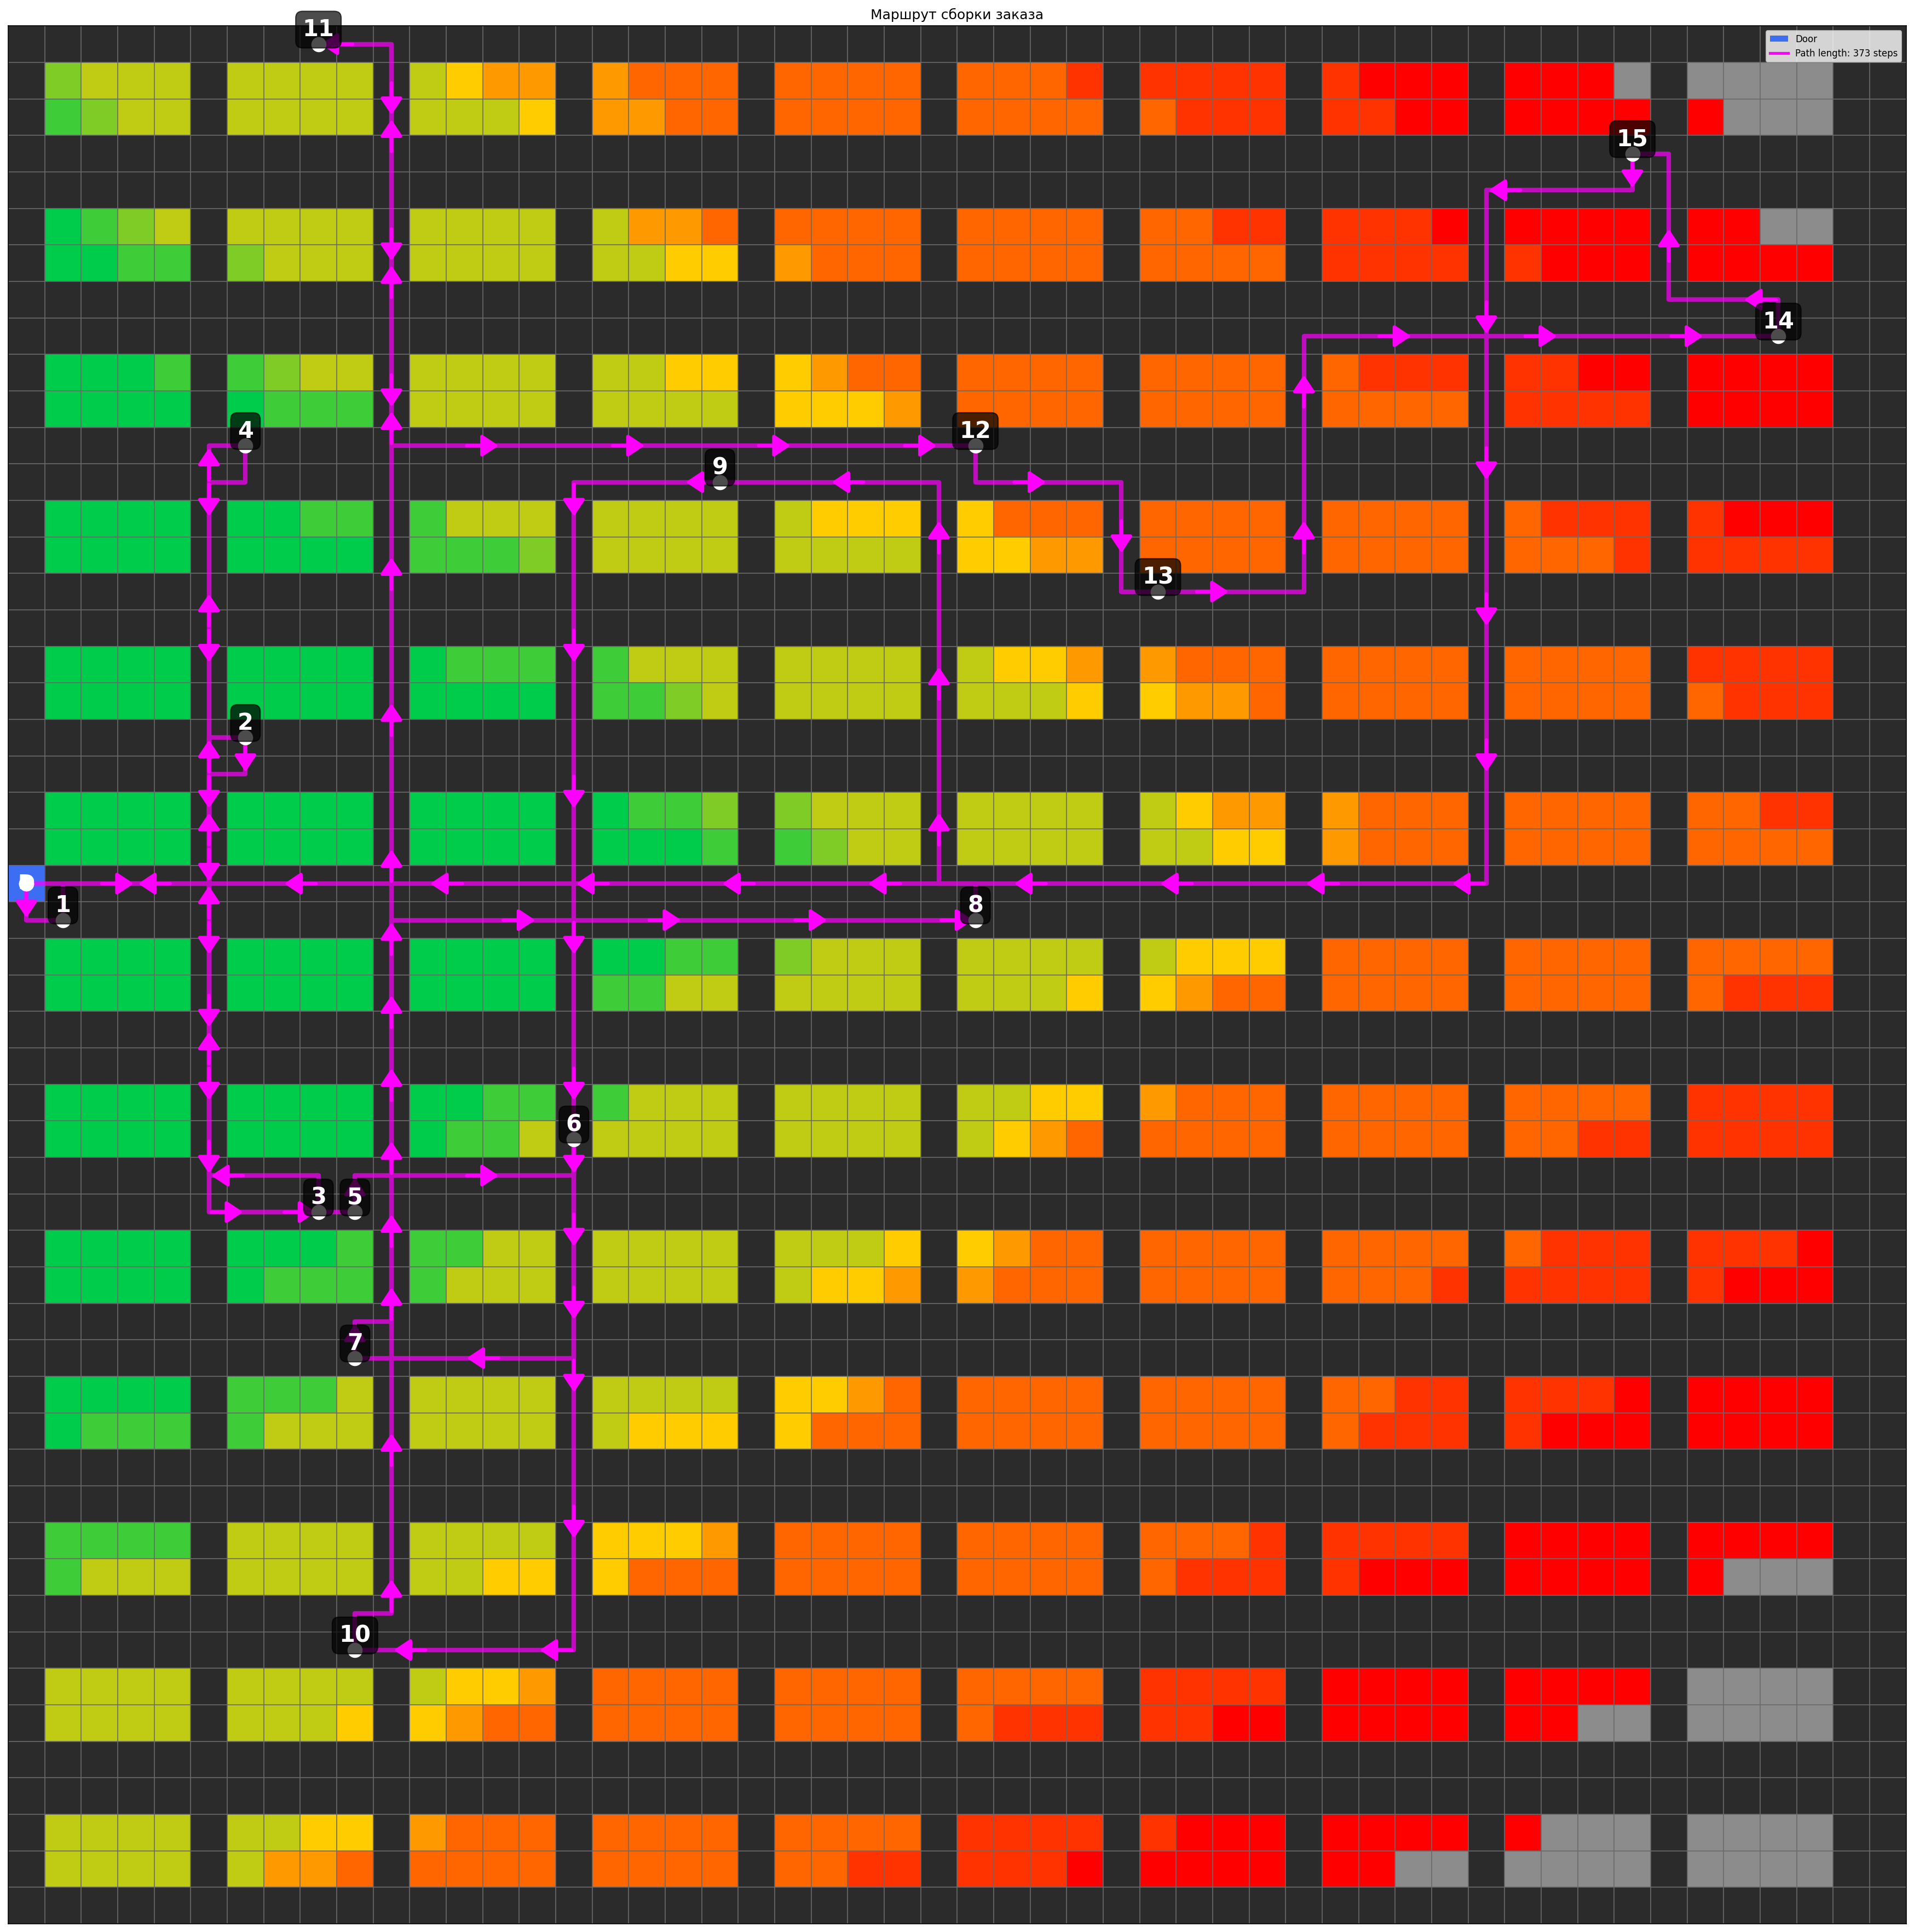
\includegraphics[width=0.8\textwidth]{order_route.png}
  \caption{Example of a picking route under the baseline model. Shelf cells are
    coloured by ABC$\times$XYZ priority (green = AX, red = CZ). The picker starts at the
    door node $v_\mathrm{door}$, visits pick locations in order of increasing BFS distance,
    and returns to the door. Numbered markers indicate the visit sequence.}
  \label{fig:route}
\end{figure}

\medskip
\noindent\textbf{Observation on Traffic Concentration.}
Even in the absence of explicit congestion modelling, the visualisation reveals repeated use
of specific aisle segments. Since high-demand SKUs are placed closer to the door and
appear more frequently in orders, the corresponding storage zones are visited repeatedly.

As a result, central corridors and areas near high-priority items experience higher traffic
intensity. This effect motivates the introduction of heat map construction and
congestion-aware routing in the extended model.

\subsubsection{Resulting Baseline Configuration}

The outcome of the two baseline components is:
\begin{itemize}
  \item A slotting configuration where each SKU $s_i \in S$ is assigned to exactly one
    shelf cell $l_j \in L$ according to ABC$\times$XYZ priority and BFS distance to the
    door (AX items closest, CZ items furthest);
  \item A routing model where all edge weights are $d_e = 1$, so the cost of each path
    equals the total number of movement steps, without any congestion penalty.
\end{itemize}

This configuration represents the simplest integrated warehouse model and serves as a
reference point for evaluating congestion-aware extensions introduced in later sections.

\subsection{2$\times$2 Experimental Design}

The $2 \times 2$ factorial design is used to measure the effect of each proposed
improvement separately. Instead of testing one combined solution, the design treats
two independent decisions --- where items are stored (slotting) and how the picker
moves between them (routing) --- as separate factors. Crossing these two factors
produces four distinct configurations. This structure allows the effect of each
change to be measured on its own and also shows what happens when both changes
are applied at the same time.

\subsubsection{Design Variables}

The two experimental factors are:

\paragraph{Slotting strategy (rows of the table).}
\begin{itemize}
  \item \textbf{Classical slotting} --- ABC$\times$XYZ placement without congestion
    awareness. High-priority AX/AY items are placed closest to the door based only
    on BFS distance.
  \item \textbf{Heat-map-informed slotting} --- ABC$\times$XYZ placement that also
    uses the observed congestion heat map. Items are moved away from zones that the
    baseline experiment identifies as structurally congested.
\end{itemize}

\paragraph{Routing strategy (columns of the table).}
\begin{itemize}
  \item \textbf{Shortest-path routing} ($\lambda = 0$) --- Dijkstra / BFS with unit
    edge weights $d_e = 1$; no congestion penalty is used.
  \item \textbf{Congestion-aware routing} ($\lambda > 0$) --- Dijkstra with the
    combined edge cost $\mathrm{Cost}(e) = d_e + \lambda\,c_e$, which penalises
    heavily used corridors and encourages detours around congested areas.
\end{itemize}

\subsubsection{Four Experimental Configurations}

Crossing the two factors yields four distinct configurations (Table~\ref{tab:2x2}):

\begin{table}[h]
\centering
\caption{$2 \times 2$ experimental design: four warehouse configurations}
\label{tab:2x2}
\begin{tabular}{lcc}
\hline
 & \textbf{Shortest-path routing} & \textbf{Congestion-aware routing} \\
\hline
\textbf{Classical slotting}   & Baseline & Config~A \\
\textbf{Heat-map slotting}    & Config~B & Config~C (full integration) \\
\hline
\end{tabular}
\end{table}

\begin{itemize}
  \item \textbf{Baseline} --- ABC$\times$XYZ slotting with shortest-path routing
    ($\lambda = 0$). This is the reference configuration described in the previous
    section. All performance improvements are measured relative to it.
  \item \textbf{Config~A} (routing improvement only) --- classical slotting with
    congestion-aware routing. Item placement does not change, but the algorithm
    penalises congested edges. Structural bottlenecks near the door are expected
    to persist, since slotting is not modified.
  \item \textbf{Config~B} (slotting improvement only) --- heat-map-informed placement
    with shortest-path routing. Moving high-demand items away from the congested
    entry zone targets the main cause of traffic concentration.
  \item \textbf{Config~C} (full integration) --- heat-map slotting combined with
    congestion-aware routing. When item placement already reduces structural
    bottlenecks, the routing algorithm has more room to choose alternative
    corridors. The combination of both axes is expected to give the largest
    overall gain.
\end{itemize}

The pre-experiment hypothesis is that the gains grow from Config~A to Config~C,
but the exact magnitude depends on how the two axes interact. The experimental
sections (Sections~9 and~10) report the measured values.

\subsubsection{Evaluation Metrics}

Four metrics are used to evaluate each configuration:

\begin{enumerate}
  \item \textbf{Weighted Path Congestion (WPC)} --- the main congestion metric.
    For a picking path $P$:
    \[
      \mathrm{WPC}(P) = \sum_{e \in E(P)} c_e,
    \]
    where $c_e \in [0,1]$ is the normalised congestion weight of edge $e$ taken
    from the heat map. WPC shows how much congested corridor capacity a picking
    route uses. A lower WPC means the route avoids busy segments, which reduces
    the chance of picker delays even if the physical path is slightly longer.

  \item \textbf{Mean route length (steps)} --- the average number of movement steps
    needed to complete an order over all $K = 10{,}000$ orders:
    \[
      \overline{L} = \frac{1}{K} \sum_{k=1}^{K} |P_k|.
    \]
    This metric reflects picking time when movement speed is assumed to be constant.
    It is used as a proxy for order fulfilment efficiency.

  \item \textbf{95th-percentile route length ($L_{95}$)} --- a robustness indicator
    based on the distribution of per-order route lengths:
    \[
      L_{95} = \mathrm{Percentile}_{95}\bigl(\{|P_k|\}_{k=1}^{K}\bigr).
    \]
    While $\overline{L}$ shows average performance, $L_{95}$ shows whether a
    configuration produces very long routes for a small but notable fraction of orders.
    A decrease in $L_{95}$ across configurations means the improvement is consistent
    and not limited to simple orders.

    \textit{Note on interpretation.} In this model, congestion weights $c_e$ are
    pre-computed from the baseline simulation and stay fixed during the experiment
    (single-picker, sequential routing). Therefore, $L_{95}$ captures worst-case
    \emph{order compositions} (e.g.\ orders whose items are in distant zones) rather
    than real-time congestion between pickers working at the same time. A dynamic,
    multi-picker simulation would be needed to study the latter, and this is left
    for future work.

    \textit{Note on data partitioning.} A train/test split is not used in this
    work. All $K = 10\,000$ orders are generated from the same fixed demand
    distribution and the same random seed, so every order is an independent sample
    drawn with identical probabilities. Building the heat map and evaluating
    routing on the same set therefore does not introduce a selection bias:
    a held-out subsample would have the same expected distribution as the training
    one. A more elaborate protocol with multiple independent order samples (for
    example, $k$-fold averaging over different seeds) is left for future work.
\end{enumerate}

Together, these three metrics give a complete picture of the $2 \times 2$ design:
WPC measures congestion load, $\overline{L}$ measures average efficiency, and
$L_{95}$ checks that improvements hold even for the most demanding orders.

\subsection{Implementation and Volumetric Characteristics}
\label{sec:volumetric}

All experiments were implemented in Python~3.12 and run on a MacBook Pro
with an Apple M4 processor and $48$~GB of RAM. The full source code base
contains approximately $5\,500$ lines of Python distributed across
$28$ files (about $270$~KB of source text). The core of the implementation
is the project-specific library \texttt{warehouse/}, which provides ten
modules (\texttt{layout}, \texttt{graph}, \texttt{slotting},
\texttt{routing}, \texttt{model}, \texttt{metrics}, \texttt{viz},
\texttt{constants}, \texttt{\_\_init\_\_}, and a few helpers).
The library accounts for approximately $2\,500$ lines and $250$~KB.
The remaining files are experiment-specific scripts (sensitivity sweeps,
plot generation, results dump) and three Jupyter notebooks
(\texttt{thesis\_notebook.ipynb}, \texttt{demo.ipynb}, and
\texttt{test.ipynb}) which were used for interactive exploration and
for the iterative construction of the heat maps and figures presented
in the report.

The experimental volume is summarised as follows:
\begin{itemize}
  \item \textbf{Dataset:} $1\,000$ SKUs with $12$ months of demand
        history, sourced from the public Kaggle ABC-XYZ Classification
        Dataset~\cite{ref6}.
  \item \textbf{Warehouse:} $52 \times 52$ grid, $1\,040$ shelf cells,
        and $1\,532$ walkable cells.
  \item \textbf{Orders:} $10\,000$ orders of $15$ items each, sampled
        with demand-weighted probabilities under a fixed seed of~$42$.
  \item \textbf{Slotting strategies tested:} $7$ in total --- Baseline
        ABC$\times$XYZ, DWC, HZR, TAPS, Aisle-Balanced, AAHMS, and
        the exploratory CAS.
  \item \textbf{Routing algorithms tested:} $2$ (BFS and Dijkstra-NN);
        full $7 \times 2 = 14$ slotting--routing combinations.
  \item \textbf{Sensitivity sweeps:} $\Delta \in \{5,10,15,20,30,50\}$;
        $h \in \{0.05,\ldots,0.30\}$ ($6$ values);
        $\alpha \in \{0,0.5,1,2,3,5,10\}$;
        $f_A \in \{0.10,\ldots,0.40\}$ ($6$ values);
        $K \in \{25,50,100,150,250,400\}$;
        $\lambda \in \{1,2,5,6,7,8,10,20\}$ on Baseline;
        $\lambda \in \{0,1,2,5,10,20\}$ on CAS.
        Together these add $45$ extra configurations.
\end{itemize}

A single full evaluation (one slotting combined with one routing algorithm,
across $K = 10\,000$ orders) takes about $30$--$60$~seconds on the M4
machine. Running the full $7 \times 2$ matrix together with the
$\lambda$-sweep on CAS therefore takes roughly $40$--$45$~minutes
end-to-end. Peak resident memory stays below $1$~GB; the dominant
data structures (the visit-count field on $52 \times 52$ cells, the
$10\,000$-order list, and the per-strategy heat maps) all fit
comfortably into RAM. All reported results use the fixed seed of~$42$,
so every experiment is reproducible from the published scripts and
notebooks.

%----------------------------------------------------------------------
\section{Congestion-Aware Routing: Experiment and Results}
%----------------------------------------------------------------------

\subsection{Config~A: Congestion-Aware Routing with Classical Slotting}

This section evaluates \textbf{Config~A} from the $2 \times 2$ experimental design:
classical ABC$\times$XYZ slotting (unchanged from the Baseline) combined with
congestion-aware routing ($\lambda > 0$). Config~A isolates the effect of routing
alone: item placement stays the same, and only the navigation strategy changes.

The key question is: \emph{does replacing shortest-path routing with a
congestion-penalised Dijkstra search reduce traffic on busy corridors, given that
high-demand items are still clustered near the door?}

The simulation uses the same $52 \times 52$ warehouse grid described in Section~5:
1\,000 SKUs in shelf cells, door at position $(23, 0)$, ABC$\times$XYZ slotting
with thresholds $A = 20\%$, $B = 30\%$, $X_{\mathrm{CV}} = 0.10$,
$Y_{\mathrm{CV}} = 0.25$.

\subsubsection{Baseline Traffic Heat Map}
\label{sec:configA_heatmap}

Before congestion-aware routing can be applied, the traffic pattern generated
by the standard ABC$\times$XYZ slotting must be recorded. A simulation of
$K = 10\,000$ orders with BFS routing ($\lambda = 0$) is run, and the number of
times each corridor cell is visited is counted. The result is the baseline traffic
heat map $H : V \to \mathbb{N}$ shown in Figure~\ref{fig:basic_heatmap}.

\begin{figure}[H]
  \centering
  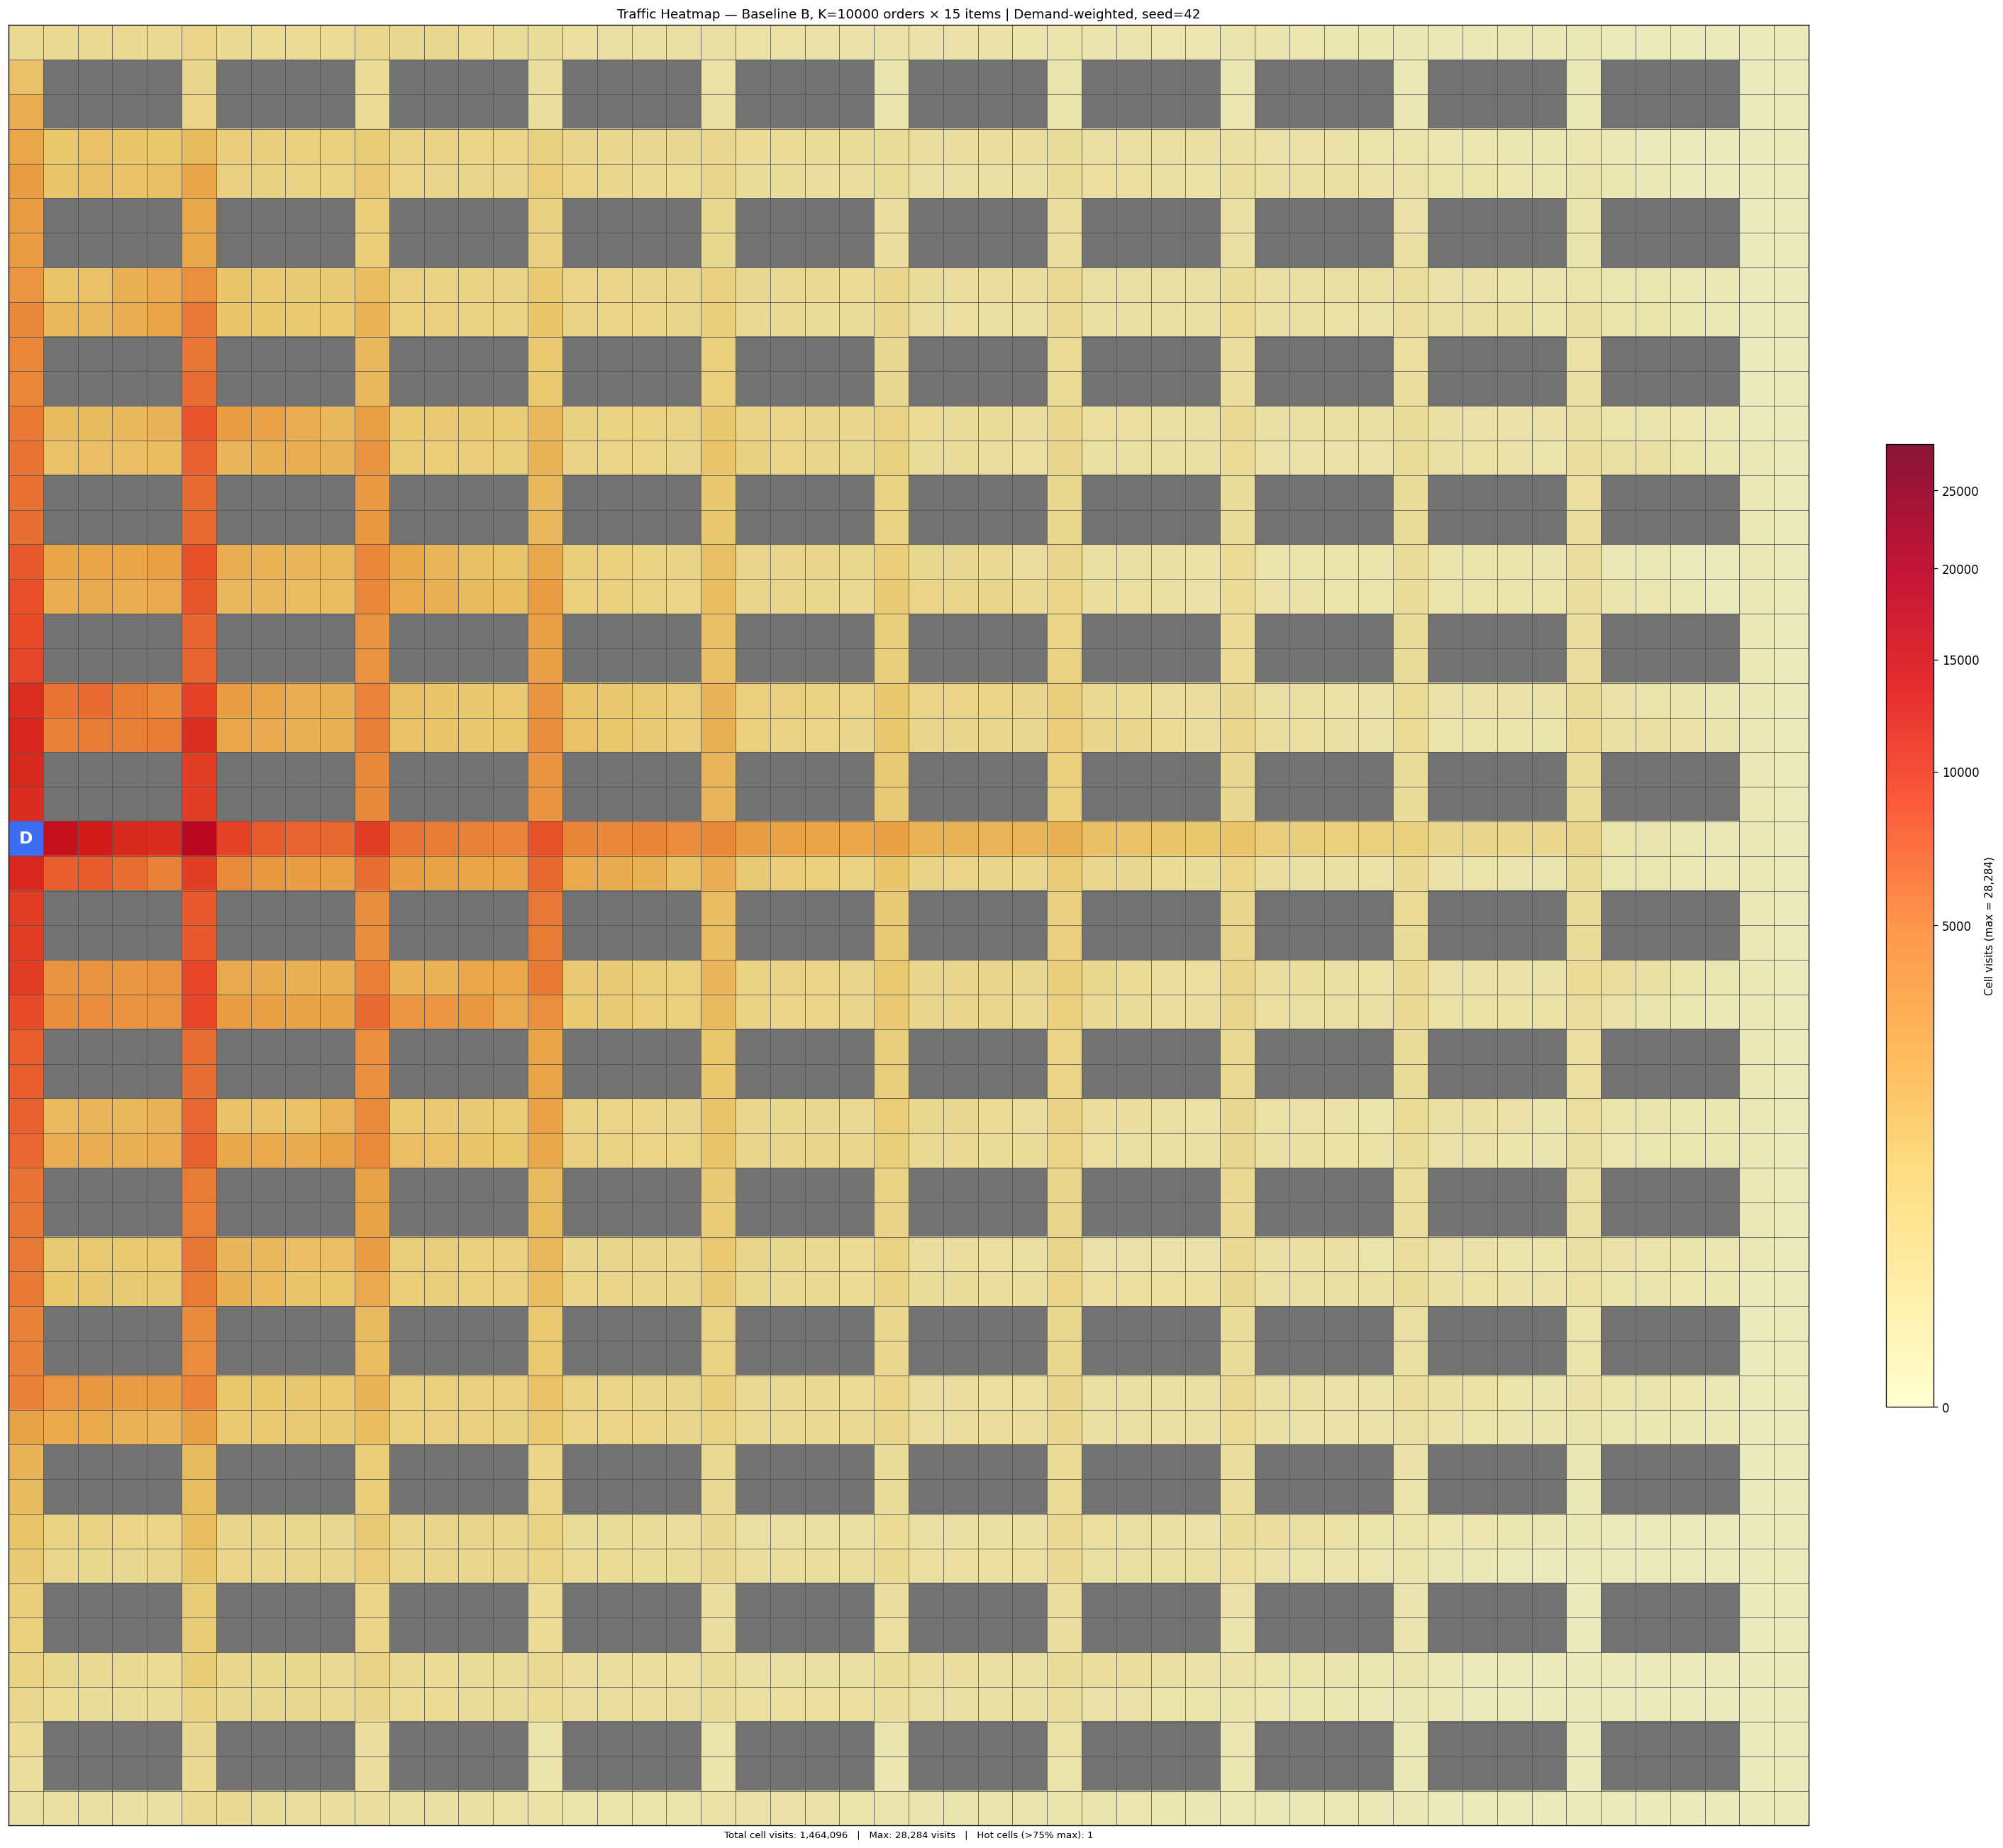
\includegraphics[width=0.80\textwidth]{basic_heatmap.png}
  \caption{Baseline traffic heat map ($K = 10\,000$ orders, BFS routing,
    demand-unit-weighted). Cell colour indicates the number of picker traversals:
    dark red is the highest load, light yellow is low load, grey cells are shelf
    blocks. The total number of cell visits is 3\,398\,472; the maximum single-cell
    count is 35\,158.}
  \label{fig:basic_heatmap}
\end{figure}

Traffic is extremely concentrated in the upper-left corner of the warehouse, near
the door. The leftmost vertical aisle and the horizontal corridor at door height act
as the primary bottleneck: every picker must pass through them to reach the A-class
shelves clustered in that zone. The rest of the warehouse --- roughly the right
two-thirds --- is barely used, with cell visit counts close to zero.

\subsubsection{Edge Congestion Weights $c_e$}

The congestion field for Config~A is built directly from the $K = 10\,000$
generated orders. Each walkable edge $e = (u, v) \in E$ collects a traversal
count, which is then normalised by the warehouse-wide maximum:
\[
  c_e = \frac{\mathrm{count}(e)}{\max_{e' \in E} \mathrm{count}(e')}, \quad c_e \in [0, 1].
\]
Edges never traversed during the simulation receive $c_e = 0$.
This congestion map is fixed and used as the static weight input to Config~A;
all reported metrics (mean steps, $L_{95}$, WPC) are computed on the same
$K = 10\,000$ orders. As explained in the note on data partitioning in
Section~5.5, a train/test split is not used here because every order is an
independent sample drawn from the same fixed distribution.

\subsubsection{Congestion-Aware Routing Algorithm}

The Baseline routes each order with a simple \emph{distance-sorted + BFS}
pipeline. Target shelves are visited in increasing order of BFS distance
from the door, and the segment between two consecutive stops is found by
an unweighted BFS.
This is a deliberately minimal routing model that uses no clever
visit-order heuristic; it serves as the simplest possible benchmark
against which the value of congestion-aware routing can be measured.

In Config~A, this pipeline is replaced by a single congestion-aware
mechanism that decides both \emph{which stop to visit next} and
\emph{how to reach it}, using the same edge cost everywhere:
\[
  \mathrm{Cost}(e) = 1 + \lambda \cdot c_e, \quad \lambda = 5.0,
\]
where $c_e \in [0,1]$ is the pre-computed normalised congestion weight of
edge~$e$.
With $\lambda = 5$, a maximally congested edge is penalised as heavily as
five additional movement steps, which strongly encourages the algorithm
to take detours around hot spots.

The routing procedure is the Dijkstra-driven nearest-neighbour heuristic
(\emph{Dijkstra-NN}):
\begin{enumerate}
  \item At the picker's current position $p$ (initially the door), run a
        single-source Dijkstra with the cost above.
        In one pass this returns the cost-distance from $p$ to every cell
        in the warehouse.
  \item Among the remaining unvisited stops, pick the one with the
        \emph{lowest Dijkstra cost} from $p$.
  \item Rebuild the path to that stop from the Dijkstra predecessor map,
        append it to the route, and update $p$ to the new position.
  \item Repeat steps 1--3 until every stop has been visited; finally
        compute one more Dijkstra from the last stop back to the door.
\end{enumerate}
The key property of Dijkstra-NN is \emph{metric consistency}: the same
$1 + \lambda c_e$ cost decides both the visit order (greedy by Dijkstra
distance from the current position) and the path between consecutive
stops.
A static sort by door distance --- the equivalent of the Baseline's
visit order --- would use one metric in the outer loop and a different
metric in the inner Dijkstra, and could send the picker through a hot
corridor on a ``shorter-by-door'' detour.
Dijkstra-NN aligns the two metrics and recomputes the order after every
visit, so that congestion penalties affect \emph{which} item is picked
next, not just \emph{how} the picker reaches an item that has already
been chosen.

\paragraph{On the choice of visit-order heuristic.}
Ratliff and Rosenthal~\cite{ref_ratliff} present a polynomial-time
dynamic-programming algorithm for the joint visit-order-and-path problem,
but only under strict topological assumptions: a single-block rectangular
warehouse with parallel aisles and a fixed depot.
The $52 \times 52$ grid used here does not meet those assumptions: shelf
rows are arbitrary, the depot lies on the perimeter, and paths may take
any shape on the full adjacency graph.
R\&R's DP is therefore not directly applicable in this study.
The survey by Petersen~\cite{ref_petersen} compares single-depot routing
heuristics (S-shape, largest-gap, NN) and reports that NN is typically
within $10$--$15\%$ of structured strategies on rectangular layouts.
Because of the topology gap above, neither S-shape nor largest-gap can be
used on the present grid without modification, so the comparison in this
work is restricted to Baseline (distance-sorted) versus Config~A
(Dijkstra-NN).

Route length alone does not show the \emph{quality} of a path in terms
of congestion: a longer route through empty corridors may be better than
a shorter route through a hot spot. The Weighted Path Congestion (WPC)
metric, defined in Section~7, captures this trade-off directly.

Table~\ref{tab:wpc} shows route lengths and WPC values for both the Baseline and
Config~A for two representative orders discussed in the following subsections.

\begin{table}[h]
\centering
\caption{Route length and Weighted Path Congestion for two orders}
\label{tab:wpc}
\begin{tabular}{lrrrrr}
\hline
\textbf{Order} & \textbf{Routing} & \textbf{Steps} & \textbf{$\Delta$Steps} & \textbf{WPC} & \textbf{$\Delta$WPC} \\
\hline
Order $o_0$ (random) & Baseline (distance-sort + BFS) & 361 & ---             & 108.58 & ---                    \\
Order $o_0$ (random) & Config~A (Dijkstra-NN, $\lambda=5$) & 249 & $-31.0\%$  & 24.89 & $-77.1\%$              \\
\hline
Typical order        & Baseline (distance-sort + BFS) & 147 & ---             & 55.86 & ---                    \\
Typical order        & Config~A (Dijkstra-NN, $\lambda=5$) & 85  & $-42.2\%$  & 16.79 & $-69.9\%$              \\
\hline
\end{tabular}
\end{table}

\subsection{Representative Orders}

The analysis uses two representative orders that cover opposite ends of the demand
spectrum:

\begin{itemize}
  \item \textbf{Order $o_0$ (randomly selected)} --- the first order generated by the
    simulation. Its 20~items are drawn from the full demand
    distribution and span several shelf zones, making it a typical example of a
    spatially dispersed order.

  \item \textbf{Typical order} --- a synthetic order composed of the 15~SKUs with the
    highest demand frequency across all 10\,000~simulated orders. Because these items
    belong to the A-class and are stored in the zone directly adjacent to the door,
    this order represents the most common traffic pattern in the warehouse and puts
    maximum stress on the entry corridor.
\end{itemize}

Figure~\ref{fig:routes_2x2} shows the four picking routes: Baseline (BFS) and
Config~A (congestion-aware, $\lambda = 5.0$) applied to each order. Shelf cells are
coloured by ABC$\times$XYZ priority (green = AX/high-demand, orange = CZ/low-demand).
The magenta line is the picking route; the letter \textbf{D} marks the door.

\begin{figure}[H]
  \centering
  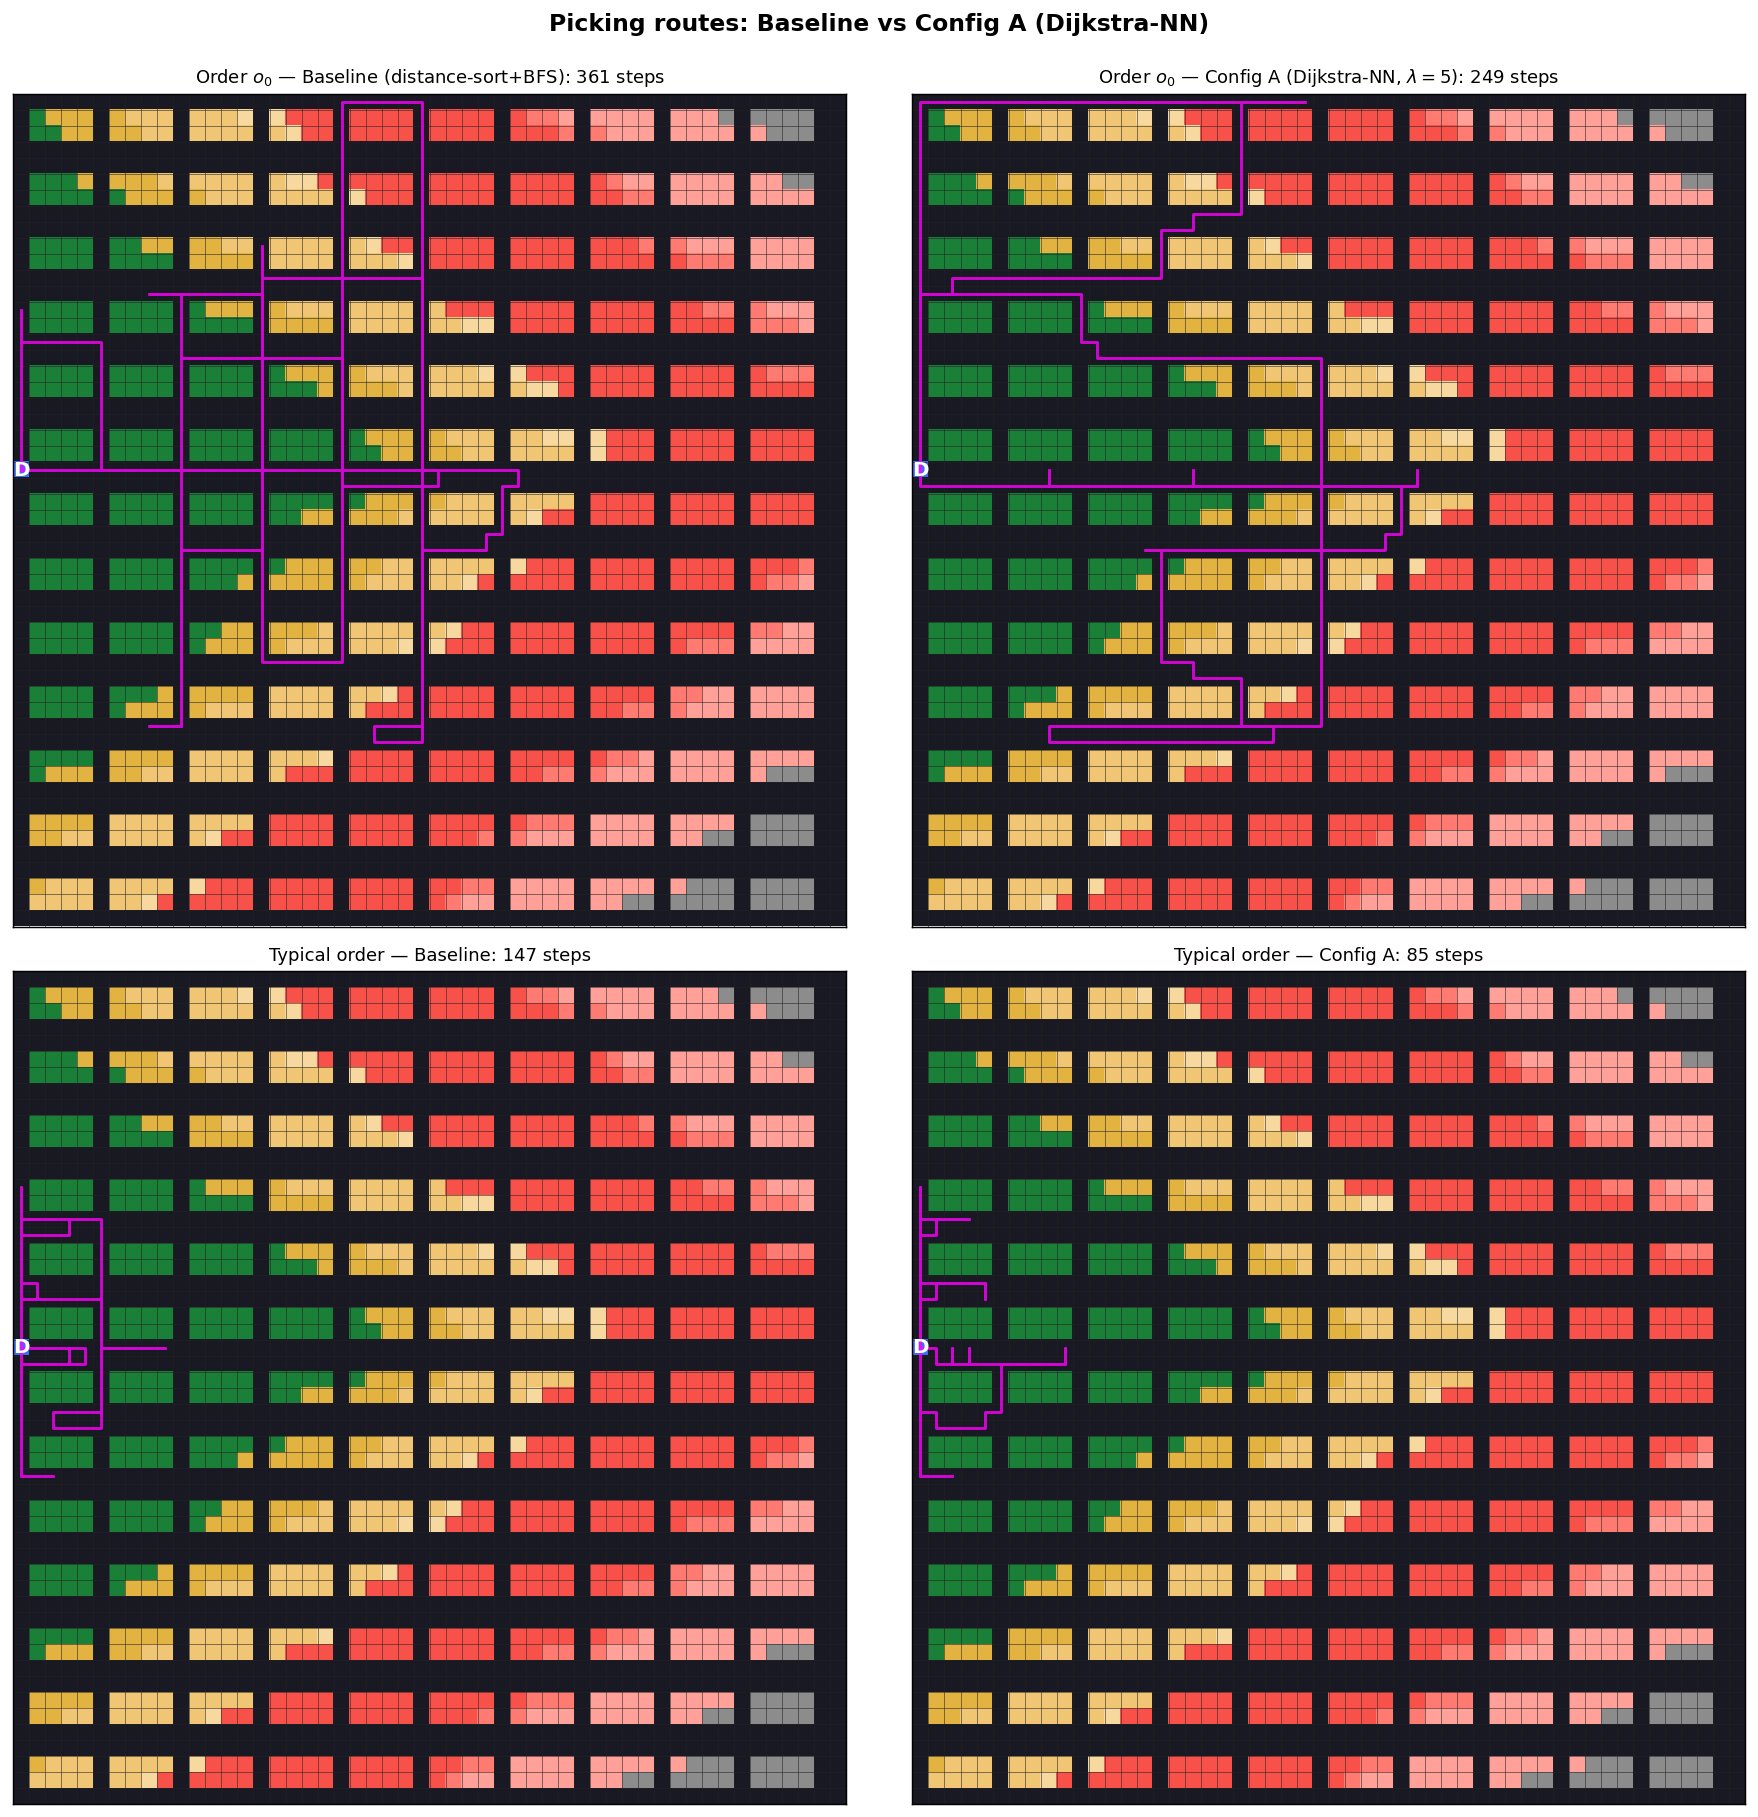
\includegraphics[width=\textwidth]{fig_routes_2x2.png}
  \caption{Picking routes for the two representative orders under BFS (left column)
    and congestion-aware routing with $\lambda = 5.0$ (right column). Top row:
    order~$o_0$ (random). Bottom row: typical order (top-15 most frequent items).
    Shelf cells are coloured by ABC$\times$XYZ category. The magenta line shows
    the picking path; \textbf{D} marks the door.}
  \label{fig:routes_2x2}
\end{figure}

To complement the route visualisations, Figures~\ref{fig:zone_order0} and
\ref{fig:zone_typical} present a \emph{zone analysis} of each order: every
walkable cell is classified by which routing algorithms use it.
\textbf{Green} cells are used by the Baseline but avoided by Config~A
(\emph{relieved by CA}); \textbf{blue} cells are CA-only detours; \textbf{red}
cells are shared by both routes (\emph{bottleneck}).
This view makes explicit \emph{where} the Dijkstra-NN router achieves its
savings.

\begin{figure}[H]
  \centering
  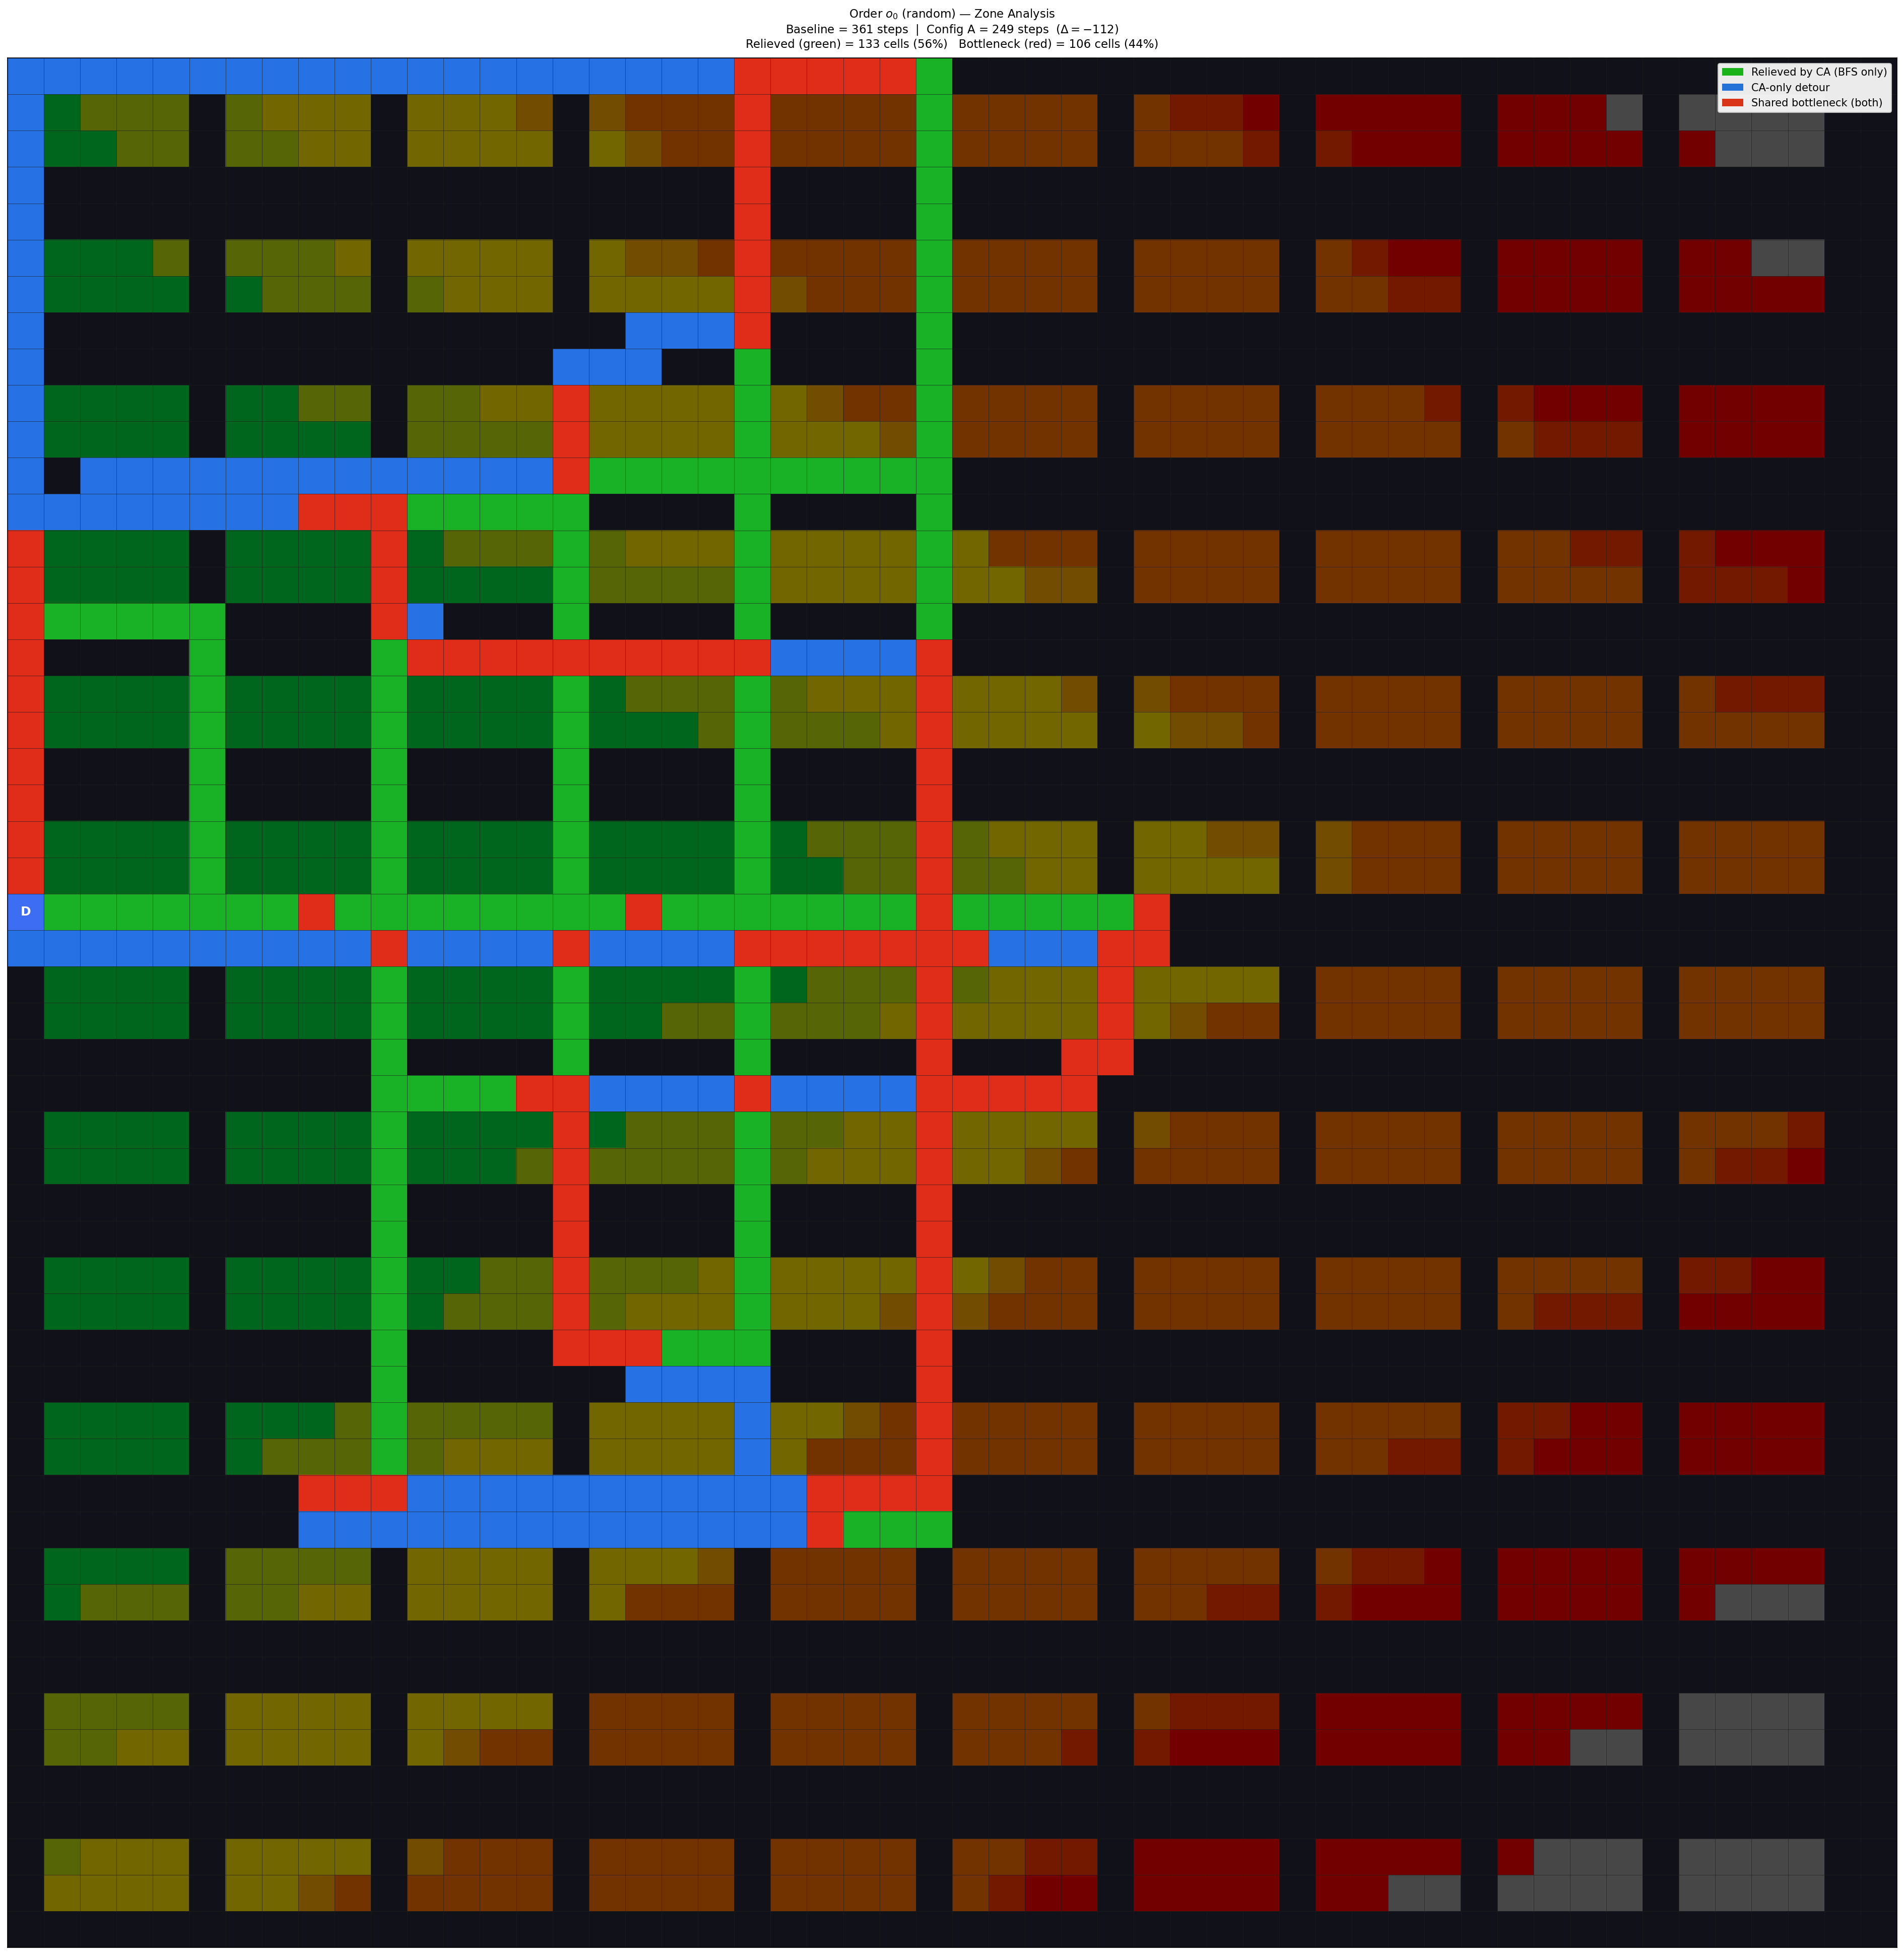
\includegraphics[width=0.85\textwidth]{fig_zone_order0.png}
  \caption{Zone analysis for order $o_0$ (random).
    Baseline route = $361$~steps, Config~A route = $249$~steps ($\Delta=-112$).
    A substantial fraction of Baseline-only cells are relieved by CA;
    a shared bottleneck remains along the entry corridor that every A-class
    pick must cross.
    Shelves are tinted by ABC$\times$XYZ category (dark green~AX
    $\to$ dark red~CZ) for spatial reference.}
  \label{fig:zone_order0}
\end{figure}

\begin{figure}[H]
  \centering
  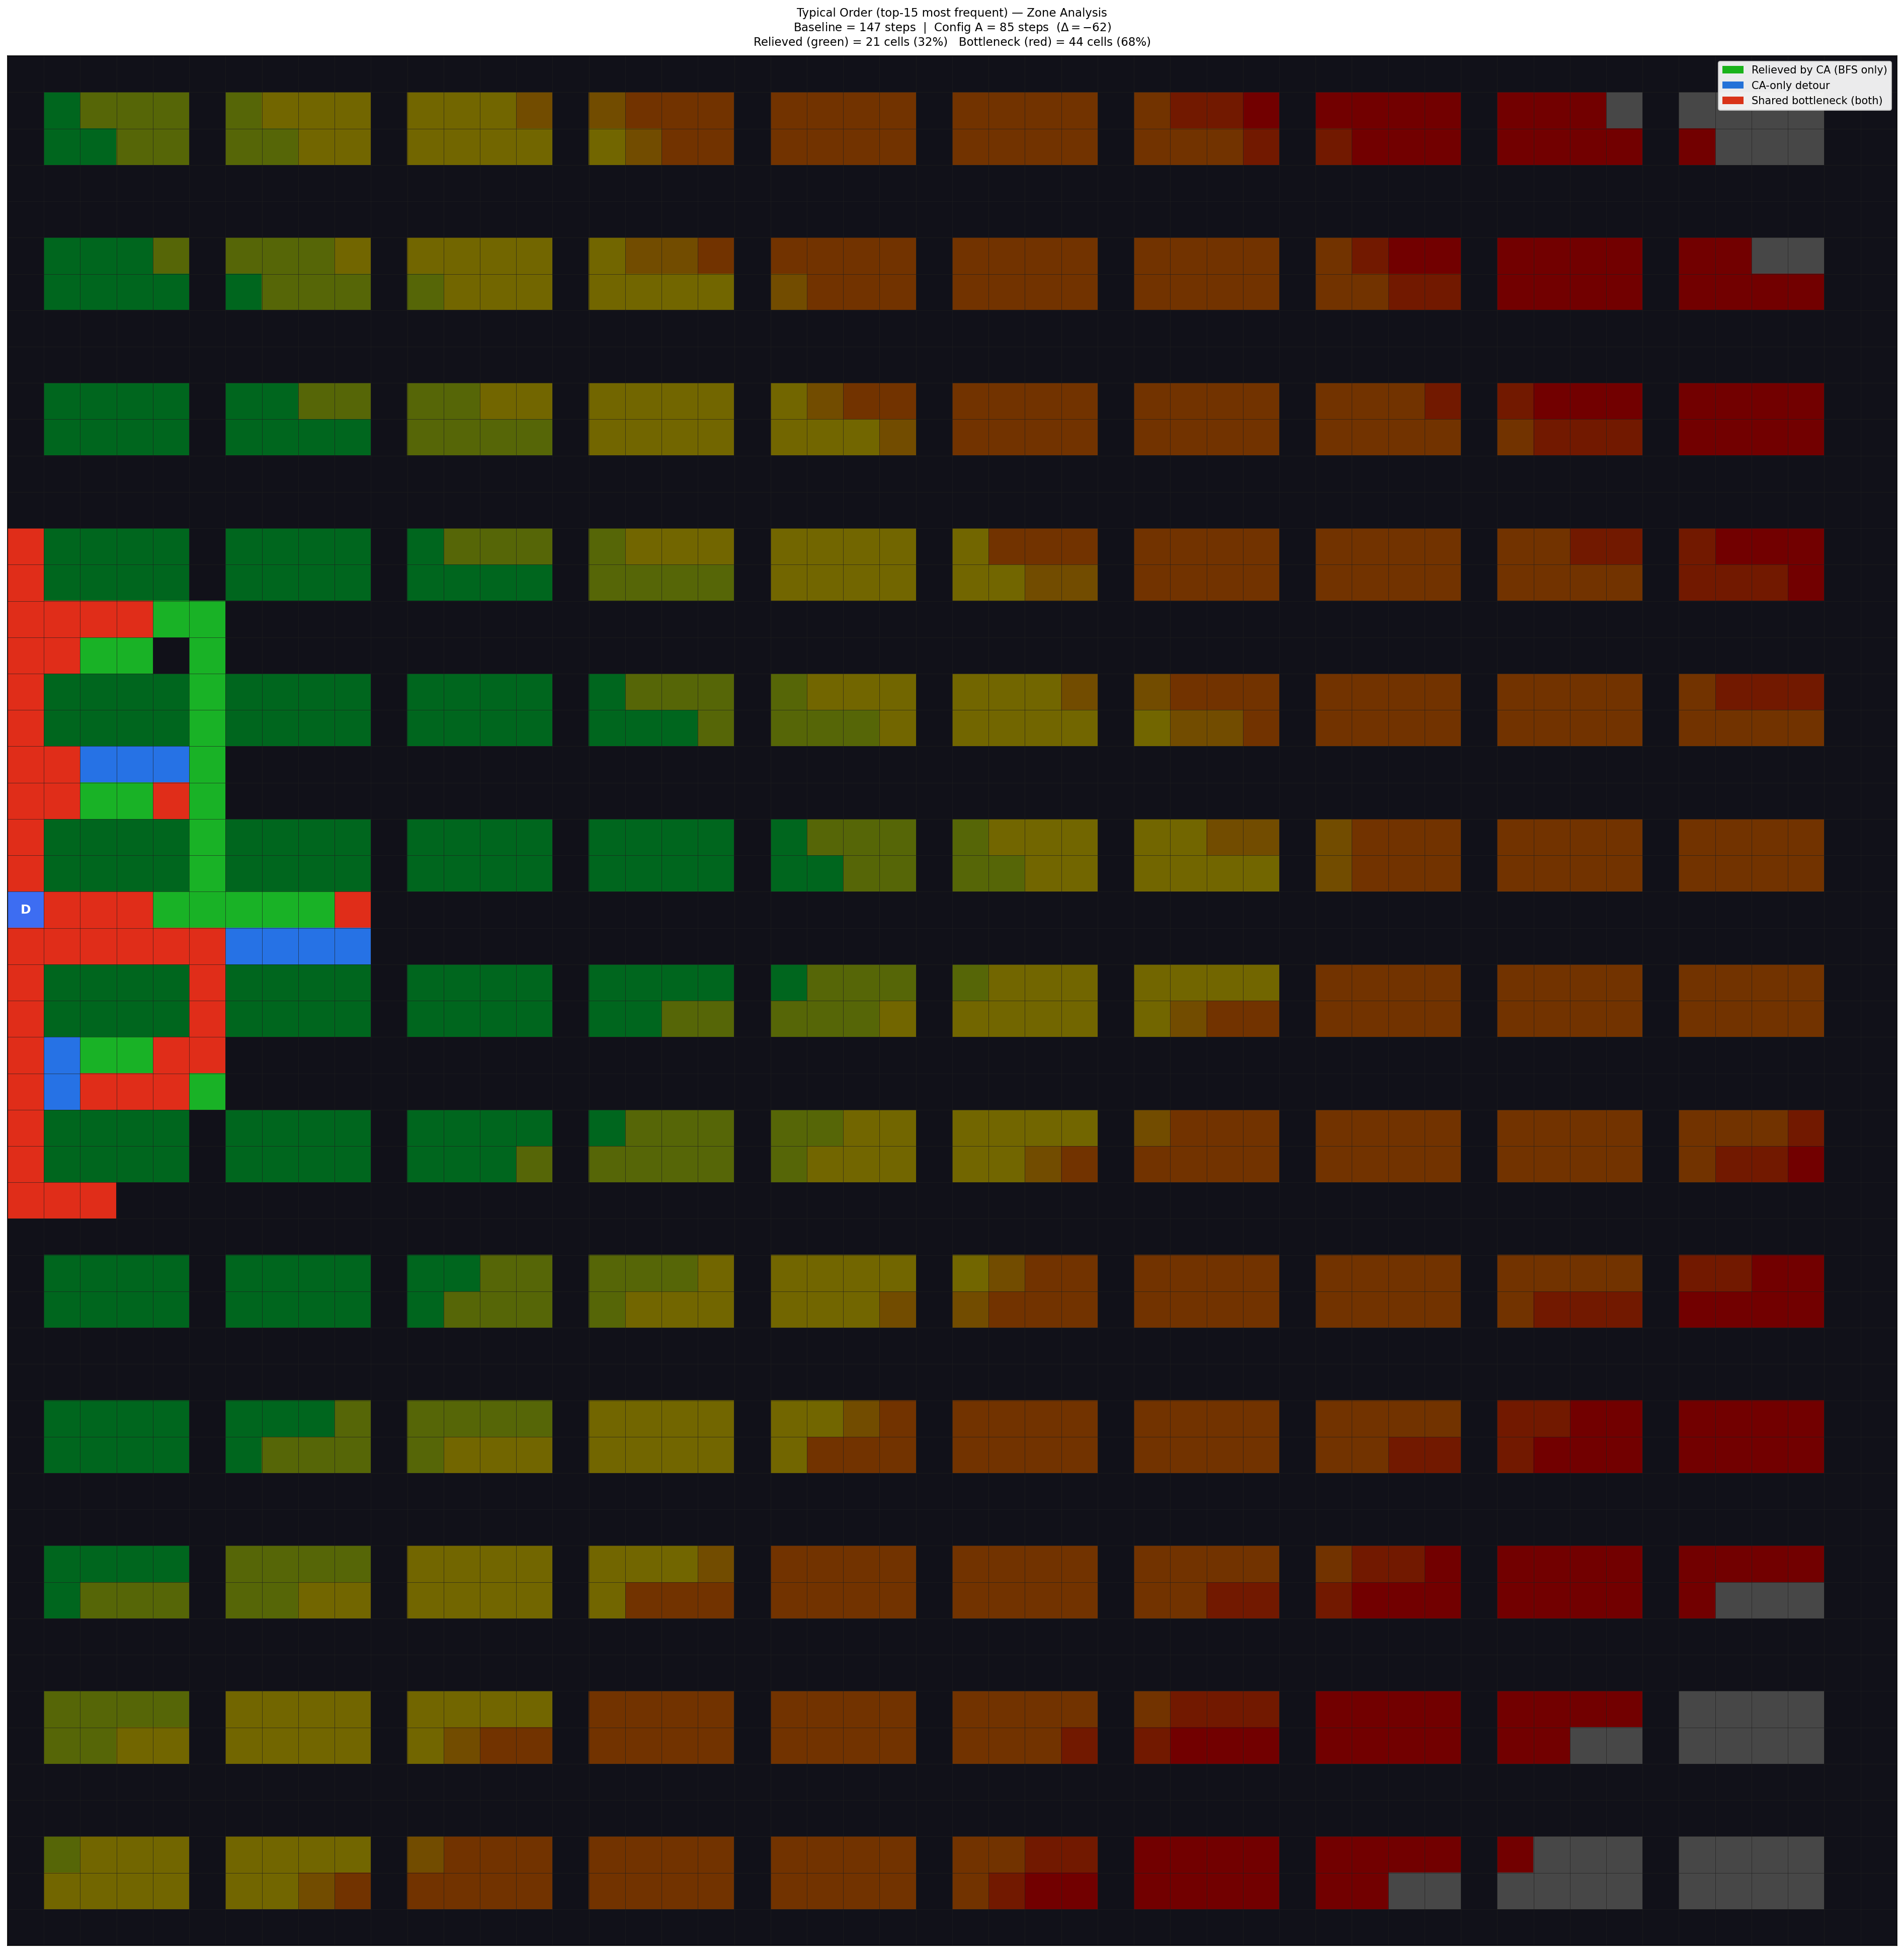
\includegraphics[width=0.85\textwidth]{fig_zone_typical.png}
  \caption{Zone analysis for the typical order (top-15 most frequent SKUs).
    Baseline route = $147$~steps, Config~A route = $85$~steps ($\Delta=-62$).
    A portion of corridor cells are relieved while the door-adjacent edges
    shared by every A-class pick remain a shared bottleneck.
    CA still finds alternative paths that shorten the route by $62$~steps
    relative to the Baseline.}
  \label{fig:zone_typical}
\end{figure}

\subsection{Results}

\paragraph{Random order $o_0$.}
On the randomly selected order, Config~A reduces the route from $361$ to
$249$~steps ($-31.0\%$) and the WPC from $108.58$ to $24.89$ ($-77.1\%$).
The metric consistency of Dijkstra-NN is the key factor: because both the
visit-order and the path-finding use the same $1 + \lambda c_e$ cost,
detours around congested edges are only taken when they also shorten the
door-relative cost. The algorithm never chooses a clean detour that
happens to be longer in practice than the cheapest non-detour.

\paragraph{Typical order.}
On the typical order --- the 15 most frequently requested SKUs, all from
the A-class zone next to the door --- Config~A reduces the route from
$147$ to $85$~steps ($-42.2\%$) and the WPC from $55.86$ to $16.79$
($-69.9\%$).
The improvement is structurally limited: every pick in the typical order
must still cross the entry corridor at least once, so the remaining WPC
of $16.79$ reflects the unavoidable load on the door-adjacent edges
themselves and not any weakness of the router.
This remaining load is exactly the part that only a change in slotting
can remove, which is the motivation for Section~9.3.

\paragraph{Aggregate metrics over $K = 10\,000$ orders.}
Across the full order set, Config~A produces routes that are on average
$34.7\%$ shorter than the distance-sorted BFS Baseline; $L_{95}$ falls from
$439$ to $281$~steps ($-36.0\%$).
Mean WPC drops from $108.50$ to $24.57$ ($-77.4\%$).
Both operational criteria (see Section~9.3.6) are therefore satisfied by
routing alone: the entry corridor is still the busiest single edge in the
warehouse, but the average picker crosses it on a path that is shorter
and less overloaded than the BFS reference.
Table~\ref{tab:metrics_aggregate} gives the full numerical summary.

\begin{table}[!ht]
\centering
\caption{Aggregate metrics: Baseline vs Config~A ($K = 10\,000$ orders,
  seed~$42$, $\lambda = 5.0$). Both routers use the same heat map built
  from the Baseline traffic.}
\label{tab:metrics_aggregate}
\begin{tabular}{lrrr}
\hline
\textbf{Config} & \textbf{Mean $L$} & \textbf{$L_{95}$} & \textbf{Mean WPC} \\
\hline
Baseline (distance-sort + BFS)            & $339.8$~steps & $439$~steps & $108.50$ \\
Config~A (Dijkstra-NN, $\lambda = 5.0$)   & $221.9$~steps & $281$~steps & $24.57$ \\
\hline
$\Delta$ (Config~A $-$ Baseline)          & $-117.9$ ($-34.7\%$) & $-158$ ($-36.0\%$) & $-83.93$ ($-77.4\%$) \\
\hline
\end{tabular}
\end{table}

\subsection{Discussion}
\label{sec:discussion_A}

Config~A gives a clear improvement over the Baseline routing on both
criteria at the same time: routes get shorter and WPC drops by roughly
three quarters.
Two points follow from the result.

\begin{enumerate}
  \item \textbf{Metric consistency is the key design choice.}
        The Baseline router sorts stops by static door distance and uses
        BFS between them; Config~A uses the same $1 + \lambda c_e$ cost
        for both ordering and path-finding (Dijkstra-NN).
        Once these two metrics agree, the algorithm no longer takes
        congestion detours that look short under the outer loop's
        ranking but long under the inner loop's. That mismatch is what
        creates pointless backtracking and inflates WPC without making
        the route shorter.

  \item \textbf{Routing alone cannot remove the structural bottleneck.}
        Even with a $-77.4\%$ drop in mean WPC, the remaining congestion on the
        typical order ($16.79$) comes mostly from the door-adjacent
        edges that every A-class pick must cross at least once.
        With demand-unit-based order sampling, class~A items account
        for $56.2\%$ of order probability mass, and the remaining B/C
        traffic reaches further shelves --- yet the entry corridor
        is on virtually every route regardless of how well the picker
        chooses the next stops.
        Routing lowers the average traversal cost of that corridor but
        cannot remove it.
\end{enumerate}

\paragraph{Implications for the $2 \times 2$ design.}
Config~A shows that the routing axis on its own makes a substantial
contribution: $-34.7\%$ mean steps and $-77.4\%$ mean WPC, simply by
replacing the visit-order heuristic with one that shares the metric of
the path-finder.
The numbers in Table~\ref{tab:metrics_aggregate} set a strong reference
against which the slotting changes (Configs~B and~C, Section~9.3) are
judged.
A slotting change only counts as a real improvement if it brings
$L_{95}$ or mean WPC below the $281$ steps and $24.57$ figures
established here.

\paragraph{Sensitivity analysis for $\lambda$.}
The penalty weight $\lambda = 5$ was chosen as a representative operating
point with moderate-to-strong detour pressure: a maximally congested
edge carries the same cost as five additional movement steps.
To check that the qualitative conclusion does not depend on this exact
choice, $\lambda$ was swept over $\{1, 2, 5, 6, 7, 8, 10, 20\}$.
Table~\ref{tab:lambda_sensitivity} reports the aggregate metrics for all
$K = 10\,000$ orders together with the WPC of the typical order.



\begin{table}[H]
\centering
\caption{Congestion-aware routing sensitivity to $\lambda \in \{1,2,5,6,7,8,10,20\}$.
  $K = 10\,000$ orders, seed~42, Dijkstra-NN throughout.
  $\Delta_L$ and $\Delta_\mathrm{WPC}$ are relative changes vs.\ Baseline ($\lambda=0$).}
\label{tab:lambda_sensitivity}
\renewcommand{\arraystretch}{1.20}
\begin{tabular}{crrrrr}
\hline
$\lambda$ & Mean $L$ (steps) & $\Delta_L$ & $L_{95}$ (steps) & Mean WPC & $\Delta_\mathrm{WPC}$ \\
\hline
Baseline (distance-sort + BFS) & 339.8 & ---       & 439 & 108.5 & ---       \\
1                              & 218.0 & $-36\%$   & 279 &  29.6 & $-73\%$   \\
2                              & 218.5 & $-36\%$   & 279 &  27.4 & $-75\%$   \\
\textbf{5}                     & \textbf{221.9} & $\mathbf{-35\%}$ & \textbf{281} & \textbf{24.6} & $\mathbf{-77\%}$ \\
6                              & 223.3 & $-34\%$   & 281 &  24.1 & $-78\%$   \\
7                              & 224.7 & $-34\%$   & 283 &  23.7 & $-78\%$   \\
8                              & 226.1 & $-33\%$   & 283 &  23.4 & $-78\%$   \\
10                             & 229.5 & $-32\%$   & 287 &  22.9 & $-79\%$   \\
20                             & 252.1 & $-26\%$   & 321 &  21.1 & $-81\%$   \\
\hline
\end{tabular}
\end{table}

The sweep shows a clean monotone trade-off rather than a scissors crossover.
Every $\lambda > 0$ tested produces routes that are shorter \emph{and} less
congested than the Baseline, simultaneously, with no degradation regime at
either extreme.
Two observations.

\emph{Route length is non-monotone.} It is minimised near $\lambda = 1$
($218.0$~steps, $-36\%$) and grows slowly with $\lambda$ thereafter.
This reflects the trade-off the parameter encodes: larger $\lambda$
buys more detour at the price of slightly longer routes.
Even at $\lambda = 5$, routes are $35\%$ shorter than Baseline
($221.9$~steps vs.\ $339.8$).

\emph{Mean WPC is monotone decreasing.} It falls from $29.6$ at
$\lambda = 1$ ($-73\%$) to $24.6$ at $\lambda = 5$ ($-77\%$) and
continues to $21.1$ at $\lambda = 20$ ($-81\%$).
Each increment of $\lambda$ buys a few more avoided hot-edge traversals,
with diminishing returns above $\lambda \approx 5$.

The selected value $\lambda = 5$ sits at the elbow of both curves:
WPC has captured $-77\%$ of the available reduction by $\lambda = 5$,
and the additional $4$~extra steps relative to the route-length minimum
at $\lambda = 1$ are a small price for the extra robustness against
heatmap noise --- at $\lambda = 1$, a $10\%$ error in any $c_e$ would
change the detour decision; at $\lambda = 5$, the same error is buried
in a much stronger congestion signal.
At $\lambda = 20$, routes grow to $252.1$~steps ($-26\%$) while WPC reaches
$21.1$ ($-81\%$) --- still below baseline on both axes, confirming the absence of
a crossover regime at any tested $\lambda$.

Figure~\ref{fig:lambda_sensitivity} illustrates the curves; the
$\lambda = 5$ operating point is marked.
Unlike the original two-metric routing model where increasing $\lambda$
helped one metric at the cost of the other (a true scissors pattern),
Dijkstra-NN eliminates the contradiction: \emph{all} positive $\lambda$
values dominate the Baseline on both axes.

\begin{figure}[H]
  \centering
  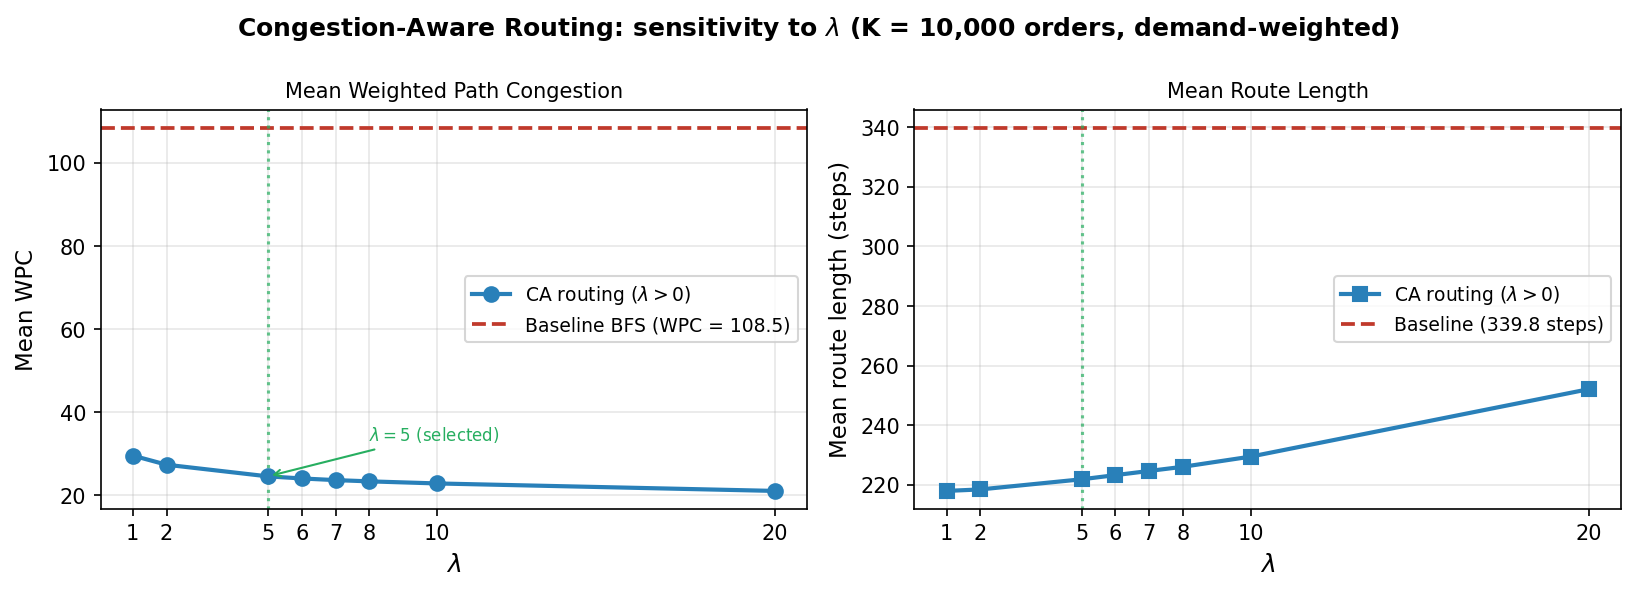
\includegraphics[width=\textwidth]{fig_lambda_sensitivity.png}
  \caption{Congestion-aware routing sensitivity to $\lambda \in \{1,2,5,6,7,8,10,20\}$
    under Dijkstra-NN (demand-unit weighted).
    Left: mean WPC over all $K=10\,000$ orders (dashed line = Baseline $108.5$).
    Right: mean route length in steps (dashed line = Baseline $339.8$~steps).
    Both metrics are below baseline at every confirmed $\lambda > 0$; the selected
    value $\lambda = 5$ sits at the elbow of both curves.}
  \label{fig:lambda_sensitivity}
\end{figure}

%----------------------------------------------------------------------
\section{Heat-Map-Informed Slotting: Experiment and Results}
%----------------------------------------------------------------------

\subsection{Config~B: Heat-Map Slotting with Shortest-Path Routing}

\subsubsection{Motivation}

In the Baseline model, the most popular items --- such as AX-class SKUs --- are
placed as close to the door as possible. This is the standard ABC$\times$XYZ
slotting rule: high-demand items should have short picking paths. In practice,
however, it creates a structural problem. Because virtually all high-frequency
orders start from the same door and immediately enter the same narrow zone,
the central entry corridors become severely overloaded. The traffic heat map
from Section~6 makes this visible: a small cluster of corridor cells near the door
receives an order of magnitude more traversals than the rest of the warehouse.

Config~A (Section~8) attempted to fix this at the routing level, but the
congestion-aware algorithm cannot bypass a bottleneck when the bottleneck is
the only gateway to the items. The root cause is the slotting decision, not the
routing logic.

\subsubsection{Heat-Map-Based Slotting Strategy}

Config~B changes the slotting algorithm instead of the routing algorithm. The
routing stays the same as in the Baseline (BFS, $\lambda = 0$); only item
placement is modified.

The key idea is that shelf attractiveness is defined not only by distance from
the door, but also by the congestion intensity of the corridors around that
shelf. A shelf that is slightly further from the door but reachable through a
quiet corridor can be a better placement for a popular item than a closer shelf
that requires passing through the most congested aisle.

\subsubsection{Iterative Algorithm}

The Config~B placement procedure works as follows:

\begin{enumerate}
  \item \textbf{Build a baseline heat map.} Starting from the standard
    ABC$\times$XYZ slotting, run $K$ orders with BFS routing and record
    the number of times each corridor cell is visited. This produces the
    traffic heat map $H : V \to \mathbb{N}$.

  \item \textbf{Identify overloaded zones.} Select the top $p\%$ of corridor
    cells by visit count (for example, $p = 20$). These are the ``hot zones''
    where congestion is highest. Shelves whose access cells fall within a hot
    zone are marked as candidates for relocation.

  \item \textbf{Relocate high-demand items.} High-demand SKUs (A-class) that
    are currently placed in hot-zone shelves are moved to quieter but still
    accessible locations (``cold-zone'' shelves). Cold-zone candidates are ranked
    by corridor congestion ascending and by BFS distance ascending, so that the
    algorithm prefers shelves that are both quiet and close to the door.

  \item \textbf{Rebuild the heat map and repeat.} After relocation, the heat map
    is recomputed to reflect the new traffic pattern. The process can be repeated
    for two or three iterations until convergence.
\end{enumerate}


The baseline traffic heat map used as the starting point for the slotting analysis
is the same one constructed in Section~\ref{sec:configA_heatmap}: $K = 10\,000$
orders routed under standard ABC$\times$XYZ slotting with BFS, yielding
the cell-visit map $H : V \to \mathbb{N}$ shown in Figure~\ref{fig:basic_heatmap}.
That heat map reveals the structural problem that motivates the slotting
strategies evaluated below.

\subsection{Identifying Overloaded Zones}

To determine which shelves are candidates for relocation, the top $p = 20\%$ of
corridor cells by visit count are selected. These are the ``hot zones'' where traffic
intensity is highest. Within this group, the top $20\%$ of the top-$20\%$ --- that
is, the top $4\%$ of all visited cells --- are classified as \textbf{critical zones}:
locations so severely overloaded that any routing strategy is almost certain to pass
through them.

In the baseline simulation, the hot-zone threshold is $1\,171$ visits per cell,
covering $307$ corridor cells ($20\%$ of the $1\,532$ active corridor cells).
The critical-zone threshold is higher still, covering the $62$ most congested cells
($4\%$ of active corridor area). These cells form the core of the entry bottleneck
and are the primary targets for slotting improvement.

Figure~\ref{fig:heatmap_hot_zones} shows the two-tier congestion map. Blue cells
are the full hot zone (top $20\%$); red cells are the critical subset (top $4\%$)
inside the hot zone. The red cluster is compact and centred directly around the
door, while the blue ring extends into the first few adjacent aisles.

\begin{figure}[H]
  \centering
  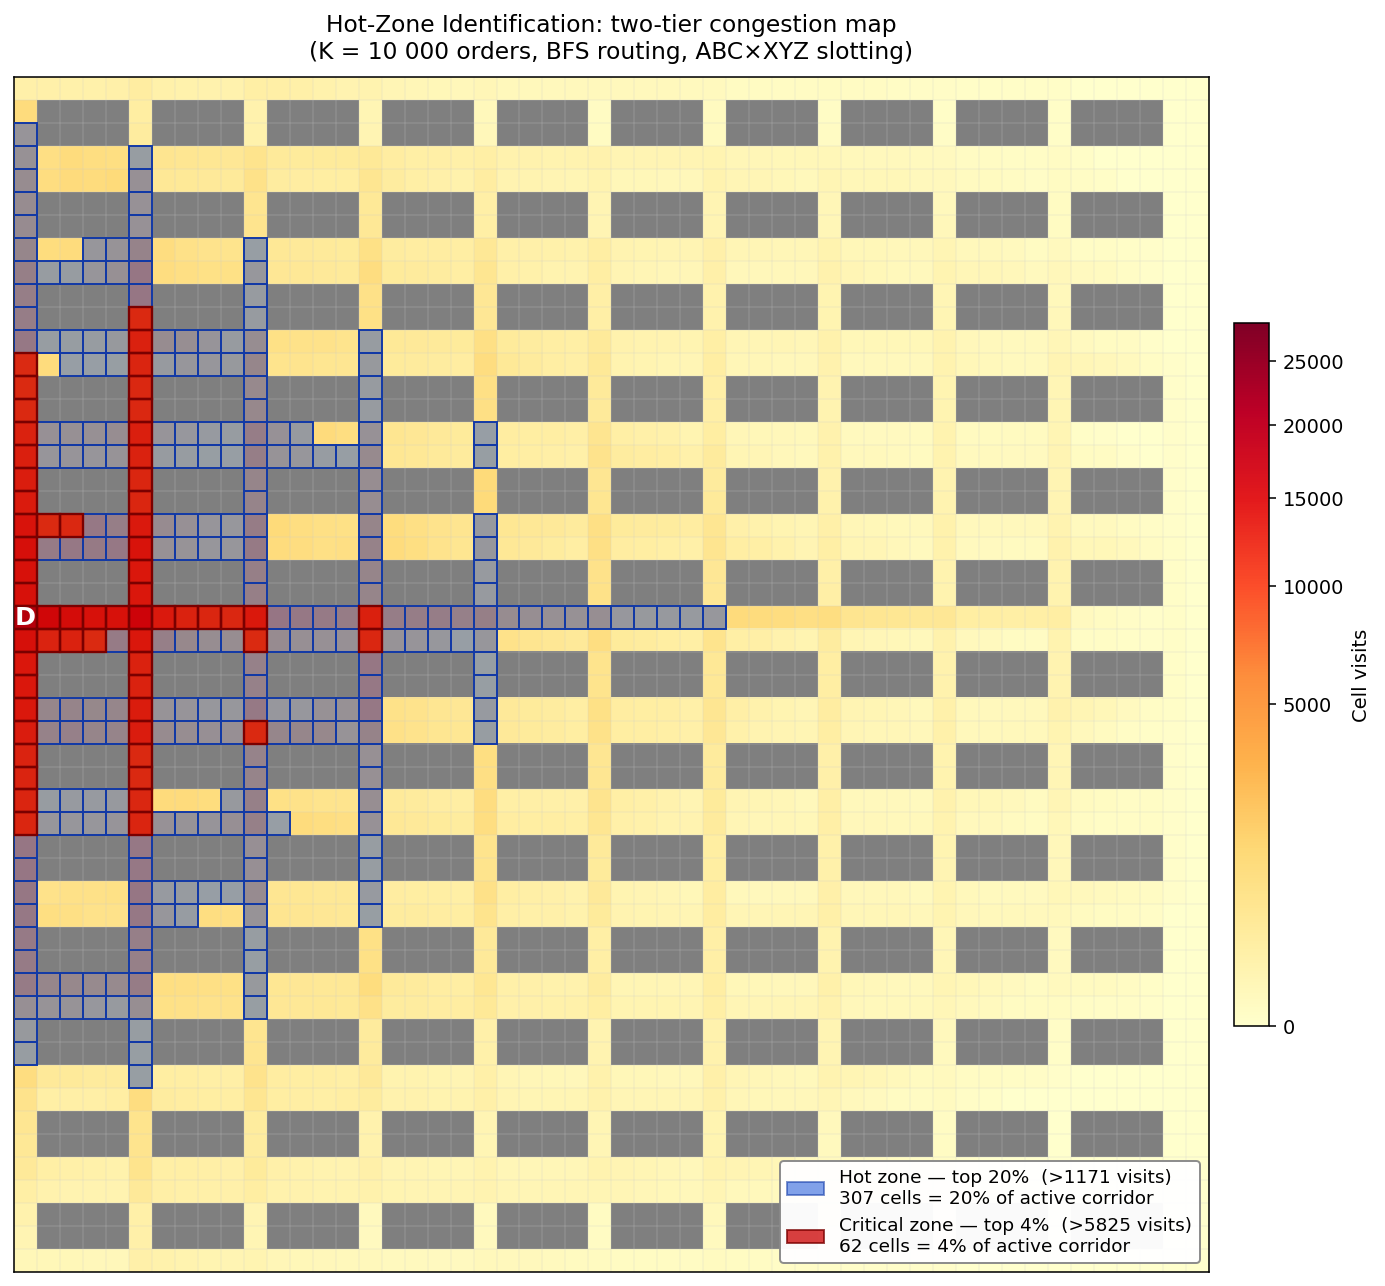
\includegraphics[width=0.85\textwidth]{fig_heatmap_hot_zones.png}
  \caption{Two-tier congestion map. Blue: hot zone (top 20% of visited corridor
    cells, $> 1\,171$ visits, 307 cells). Red: critical zone (top 20% of the hot
    zone = top 4% overall), marking the most severely congested cells directly
    around the door. These are the primary relocation targets for Config~B slotting.}
  \label{fig:heatmap_hot_zones}
\end{figure}


The two-tier map reveals an important asymmetry. The $62$ red cells (critical zone)
are not uniformly spread across the left part of the warehouse --- they form a tight
cluster in the two or three aisles immediately adjacent to the door. This is precisely
where every picking route begins and ends, so no routing change can avoid these cells
as long as the most popular items remain stored there.

\subsubsection{Why Naive Relocation Fails}

A natural first instinct is to take the A-class items from the critical-zone shelves
and move them as far from the door as possible, into the quietest corridor cells in
the warehouse. This relieves the bottleneck at the entry but creates a new problem:
every picker must now travel much further to reach those items.
\textit{(The illustrative experiment below uses revenue-weighted sampling, where baseline
Gini~$= 0.772$; the main analysis uses demand-unit weighting with baseline Gini~$= 0.670$.
The qualitative conclusion --- naive relocation reduces congestion at the cost of
dramatically longer routes --- holds under both weightings.)}

To quantify this effect, a Gini Heatmap Slotting algorithm was applied:
the top $20\%$ most congested A-class shelves were swapped with the bottom $60\%$
least-congested C-class shelves, with no distance constraint. The traffic Gini
coefficient improved by $23\%$ (from $0.772$ to $0.595$), confirming that traffic
was redistributed more evenly across the warehouse. Measured against the fixed
baseline congestion field, WPC also drops because the new routes detour around
the originally hot corridor. The cost shows up on route length:

\begin{itemize}
  \item For the typical order: WPC drops by $-38\%$ (from $30.6$ to $19.1$),
    but route length grows from $69$ to $217$ steps ($+215\%$).
  \item For order $o_0$: WPC drops by $-59\%$ (from $43.1$ to $17.7$),
    yet route length grows from $153$ to $233$ steps ($+52\%$).
\end{itemize}

\begin{figure}[H]
  \centering
  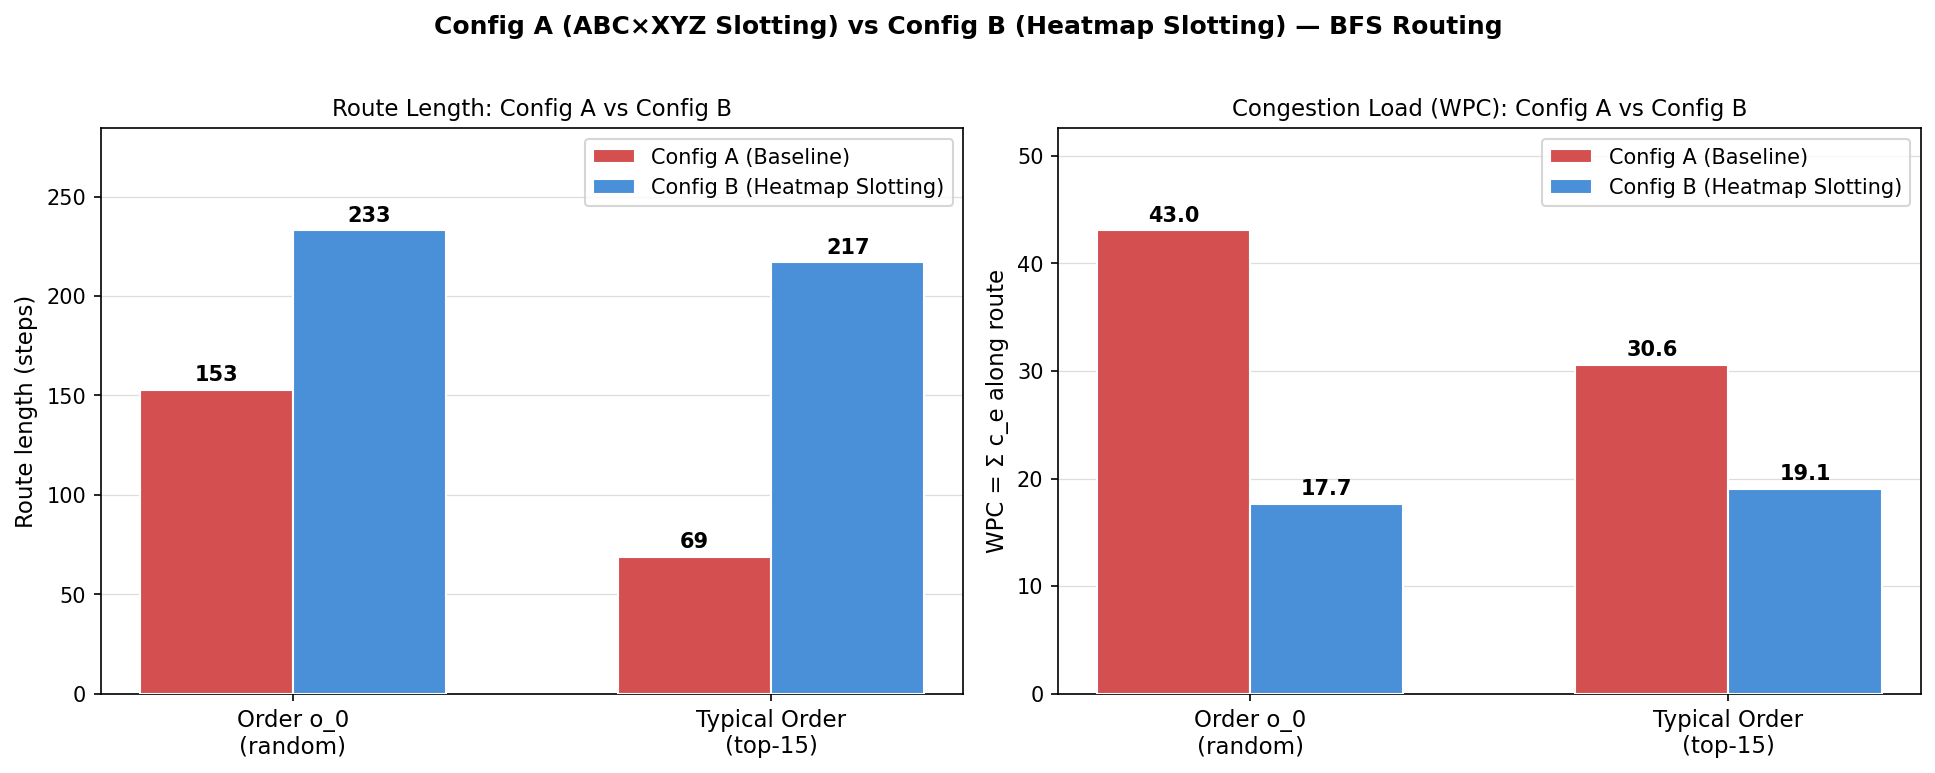
\includegraphics[width=\textwidth]{fig_naive_relocation_impact.png}
  \caption{WPC (left) and route length in steps (right) for the typical order and
    order $o_0$, before and after Gini Heatmap Slotting. Under the fixed baseline
    congestion field, WPC drops ($-38\%$ for the typical order, $-59\%$ for
    order~$o_0$) because the new routes detour around the originally hot corridor,
    but route lengths grow by $+215\%$ and $+52\%$ respectively.}
  \label{fig:naive_relocation_impact}
\end{figure}

Figure~\ref{fig:configB_heatmap_comparison} illustrates the traffic pattern before and
after Gini Heatmap Slotting. On the left, the baseline heat map shows the familiar
entry bottleneck. On the right, after relocating $179$ high-demand shelves from the
hot zone to the bottom $60\%$ of quietest positions, the entry congestion partially
disappears but a new high-traffic arc forms along the far right side and bottom
corners of the warehouse, where the relocated items now reside.

\begin{figure}[H]
  \centering
  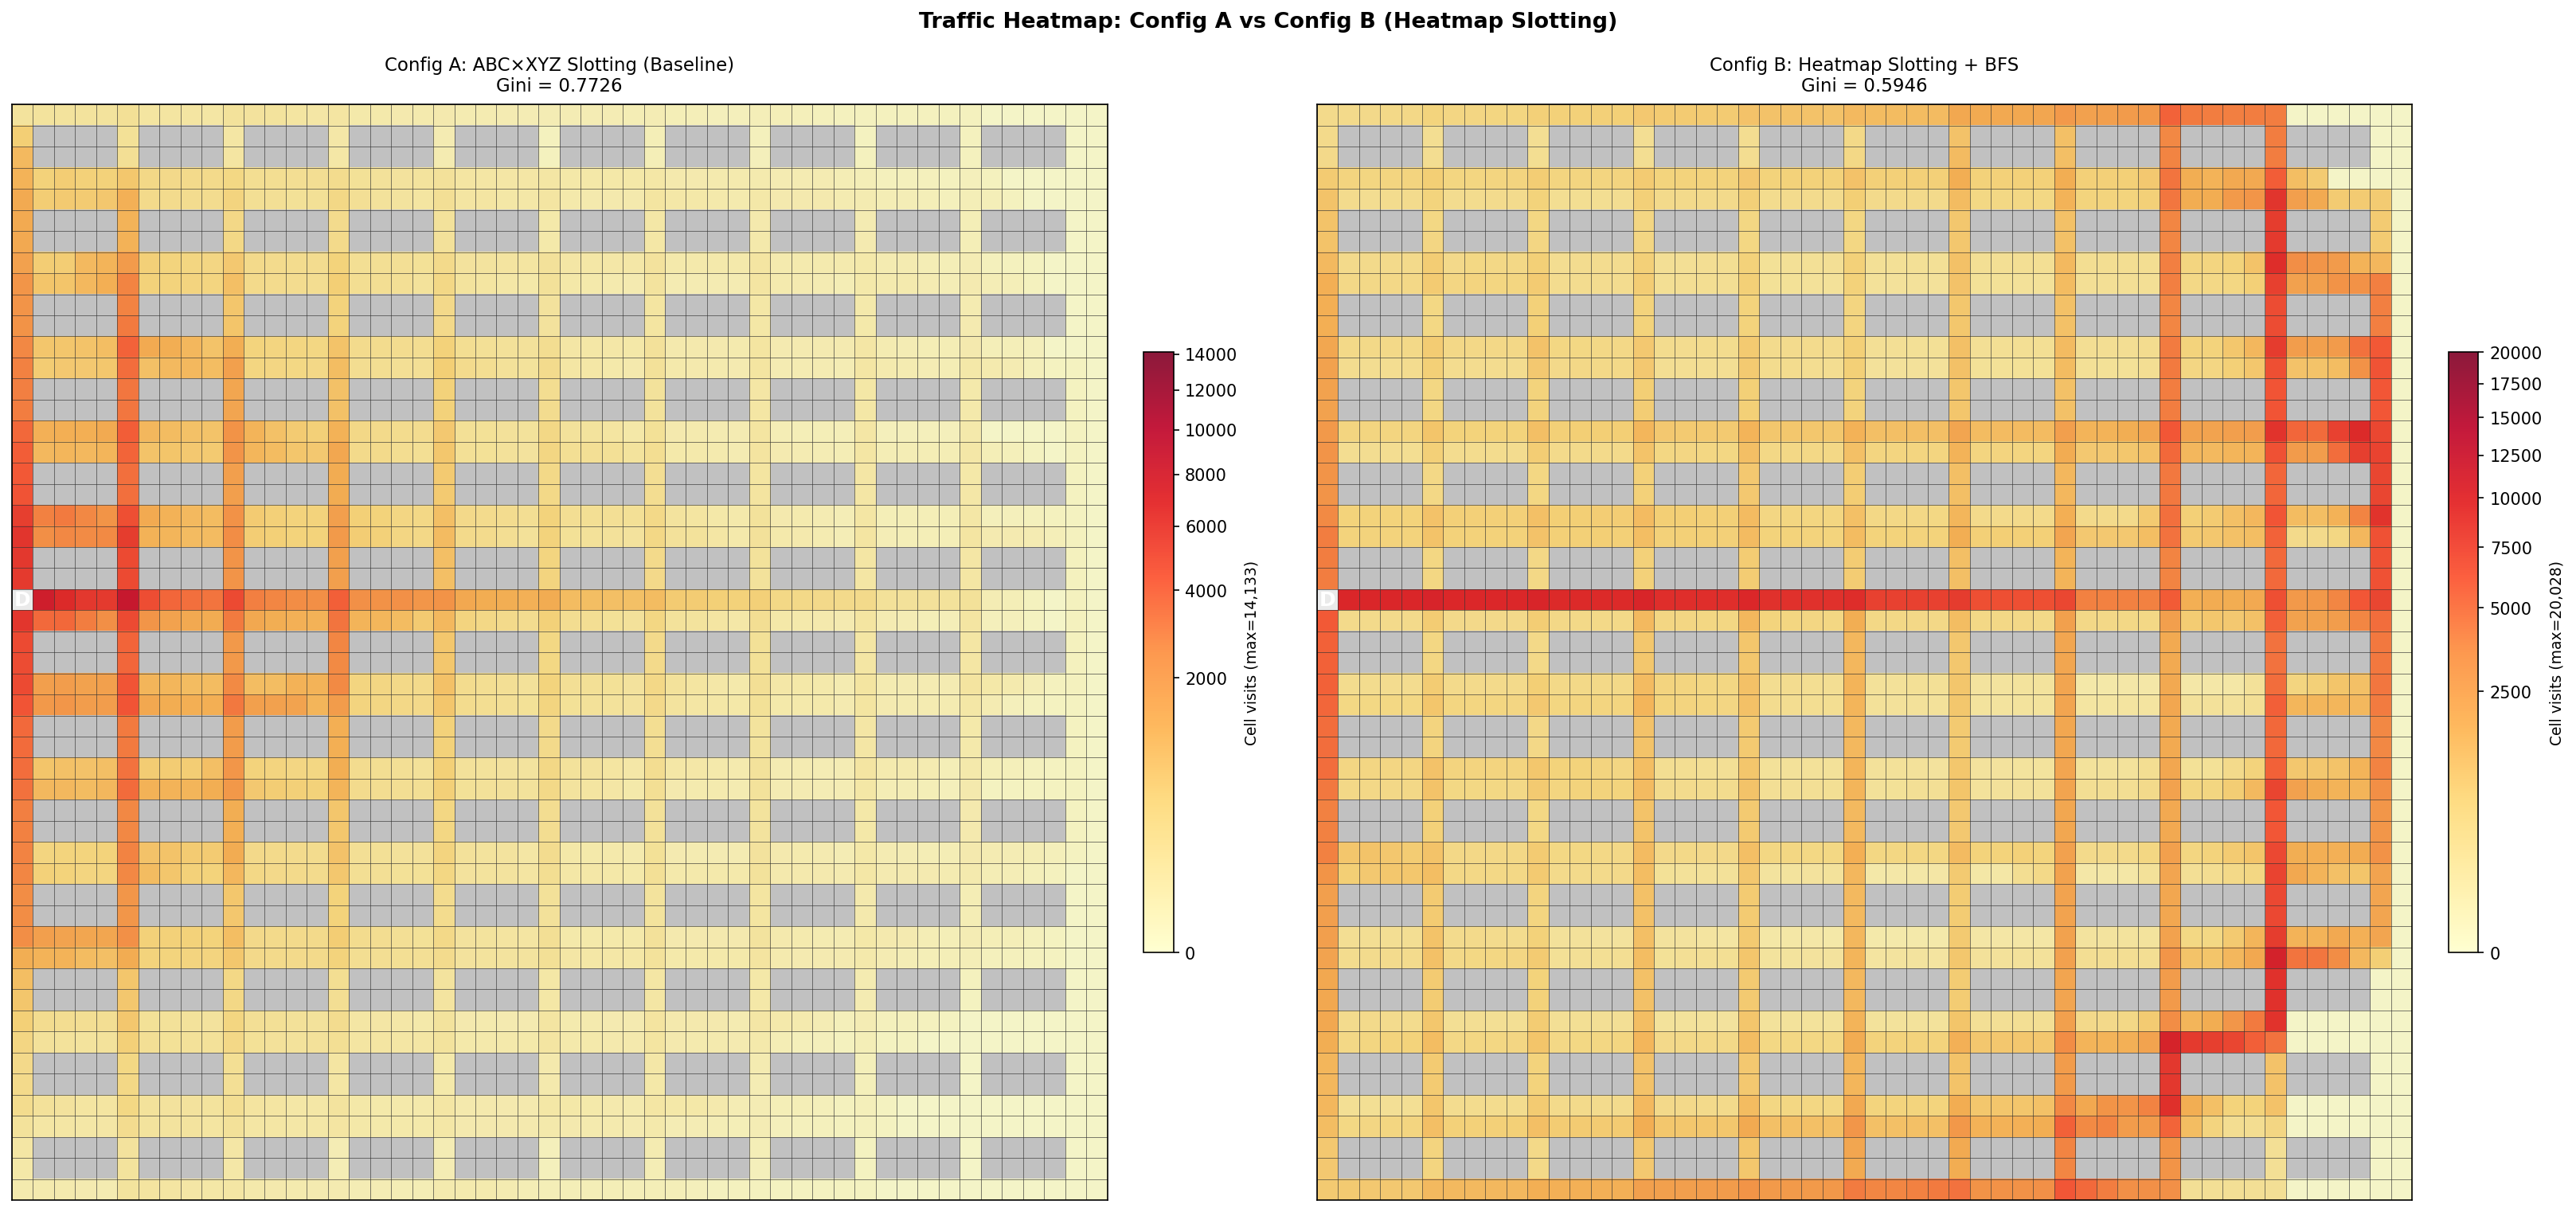
\includegraphics[width=\textwidth]{fig_configB_heatmap_comparison.png}
  \caption{Traffic heat maps before (left, Baseline Config~A) and after (right,
    Gini Heatmap Slotting) relocating the top $20\%$ most congested A-class shelves
    to the quietest $60\%$ of positions without a distance constraint.
    Gini coefficient improves from $0.772$ to $0.595$ ($-23\%$), but total cell
    visits increase from $1{,}464{,}096$ to $2{,}330{,}670$ and route length
    grows by up to $+215\%$, because every route must now travel to remote aisles.}
  \label{fig:configB_heatmap_comparison}
\end{figure}

The reason is straightforward. Displaced A-items now sit in remote aisles that were
previously rarely visited. Every order that includes an A-item must now traverse
the door-side corridors \emph{to exit the entry zone}, travel a long distance to the
remote shelf, and then return. While the new routes do bypass the originally hot
corridor (lowering WPC against the baseline congestion field), the extra travel
distance more than doubles route length, which dominates picking cost.

This result leads to a precise design criterion. A viable slotting strategy for
Config~B must satisfy two conditions simultaneously:
\begin{enumerate}
  \item \textbf{Reduce critical-zone load:} A-class items must be moved away from
    the $62$ red cells near the door, lowering peak corridor traversal counts.
  \item \textbf{Preserve route efficiency:} Relocated items must be placed at
    positions that do not significantly increase average route length, so that the
    congestion reduction along the former bottleneck is not offset by new congestion
    on longer paths.
\end{enumerate}

The following subsection evaluates five slotting algorithms against these two
criteria. Each addresses the critical zone in a different way --- from targeted
shelf swaps to full warehouse-wide reassignment --- and the simulation results
determine which strategy achieves the best outcome.

\subsection{Slotting Variant Comparison}

This subsection evaluates five slotting algorithms against the two design criteria
identified above: reducing critical-zone load and preserving route efficiency.
All five variants share the same experimental setup --- the $52\times52$ warehouse,
$1{,}000$ SKUs, and $10{,}000$ simulated orders --- and are compared against the
Baseline Config~A using BFS routing ($\lambda = 0$).
Two representative orders are used as benchmarks throughout:
\textit{Order~$o_0$}, a randomly sampled order, and the \textit{typical order},
constructed from the 15 most frequently demanded SKUs.
Metric: Weighted Path Congestion $\mathrm{WPC}(P)=\sum_{e\in E(P)}c_e$,
where $c_e$ is the edge congestion weight from the baseline heatmap.

%----------------------------------------------------------------------
\subsubsection{Strategy~1: Distance-Constrained Swap (DWC Slotting)}
%----------------------------------------------------------------------

\paragraph{Idea.}
A-class items located in the critical zone are swapped with C-class items
whose BFS distance from the door lies within a tolerance window
$|d_A - d_C| \le \Delta$, with $\Delta = 5$ steps in this experiment.
The rationale is to preserve the ABC proximity principle --- high-demand items remain
close to the door --- while dispersing them across several nearby aisles instead of
concentrating all of them in the single most-congested corridor.

\paragraph{Algorithm.}
For each A-item shelf $s_A$ in the critical zone, the procedure searches among all
C-item shelves $s_C$ satisfying $|d(s_A) - d(s_C)| \le \Delta$.
If such a shelf exists, the items are swapped and $s_A$ is removed from the
candidate set.
The heatmap is rebuilt after all swaps to capture updated edge-congestion weights.

\paragraph{Parameter sensitivity analysis.}
To verify that $\Delta = 5$ is not an arbitrary conservative choice, the tolerance
was swept over $\Delta \in \{5, 10, 15, 20, 30, 50\}$ BFS steps.
Table~\ref{tab:dwc_delta} reports the number of executed swaps, the resulting WPC
for the typical order, average route length, and Gini coefficient for each value.

\begin{table}[H]
\centering
\caption{DWC Slotting sensitivity to the distance tolerance $\Delta$.
  All metrics measured for the typical order ($K=10{,}000$ orders, seed~$42$).
  $\Delta_\mathrm{WPC}$ and $\Delta_\mathrm{len}$ are relative changes vs.\ Baseline.}
\label{tab:dwc_delta}
\renewcommand{\arraystretch}{1.20}
\begin{tabular}{ccccccc}
\hline
$\Delta$ & Swaps & WPC & $\Delta_\mathrm{WPC}$ & Steps & $\Delta_\mathrm{len}$ & Gini \\
\hline
Baseline & --- & 55.86 & ---         & 147 & ---        & 0.670 \\
5        & 0   & 55.86 & $\pm0\%$   & 147 & $\pm0\%$  & 0.670 \\
10       & 0   & 55.86 & $\pm0\%$   & 147 & $\pm0\%$  & 0.670 \\
15       & 10  & 55.86 & $\pm0\%$   & 147 & $\pm0\%$  & 0.663 \\
20       & 84  & 55.86 & $\pm0\%$   & 147 & $\pm0\%$  & 0.624 \\
30       & 182 & 42.14 & $-24.6\%$  & 197 & $+34.0\%$ & 0.577 \\
50       & 200 & 25.71 & $-54.0\%$  & 265 & $+80.3\%$ & 0.572 \\
\hline
\end{tabular}
\end{table}

The demand-weighted setup reveals a fundamentally different pattern from the
revenue-weighted one.
\emph{DWC makes zero swaps at $\Delta \le 20$} because the demand-unit-based
ABC classification already places high-demand items in near-door positions:
when items are ranked by annual units, the most-picked SKUs naturally land
in the closest shelves, leaving no overloaded critical zone that DWC needs to
correct.
At $\Delta = 15$ and $\Delta = 20$ the tolerance window is wide enough to admit
$10$ and $84$ candidate pairs respectively, but those rearrangements involve
shuffling items within the same near-door band and produce no change in WPC or
route length.
Only at $\Delta = 30$ does the relocation cross into noticeably further shelves:
route length grows by $+34\%$ (from $147$ to $197$~steps) while WPC falls by
$-24.6\%$ (from $55.86$ to $42.14$).
At $\Delta = 50$, displacement is so large that WPC drops by $-54\%$ but route
length grows by $+80.3\%$ --- the same failure mode as naive relocation.

\textbf{Observation:} DWC has nothing to improve under demand-unit weighting.
The fundamental geometric incompatibility identified under revenue weighting ---
where the A/C distance gap was smaller than the tolerance window --- disappears:
the demand-based slotting creates a tight near-door cluster that DWC cannot
break up without also increasing route length.
Strategy~1 therefore produces \emph{no net gain at any tested parameter value}
without violating the route-efficiency constraint.

\begin{figure}[H]
  \centering
  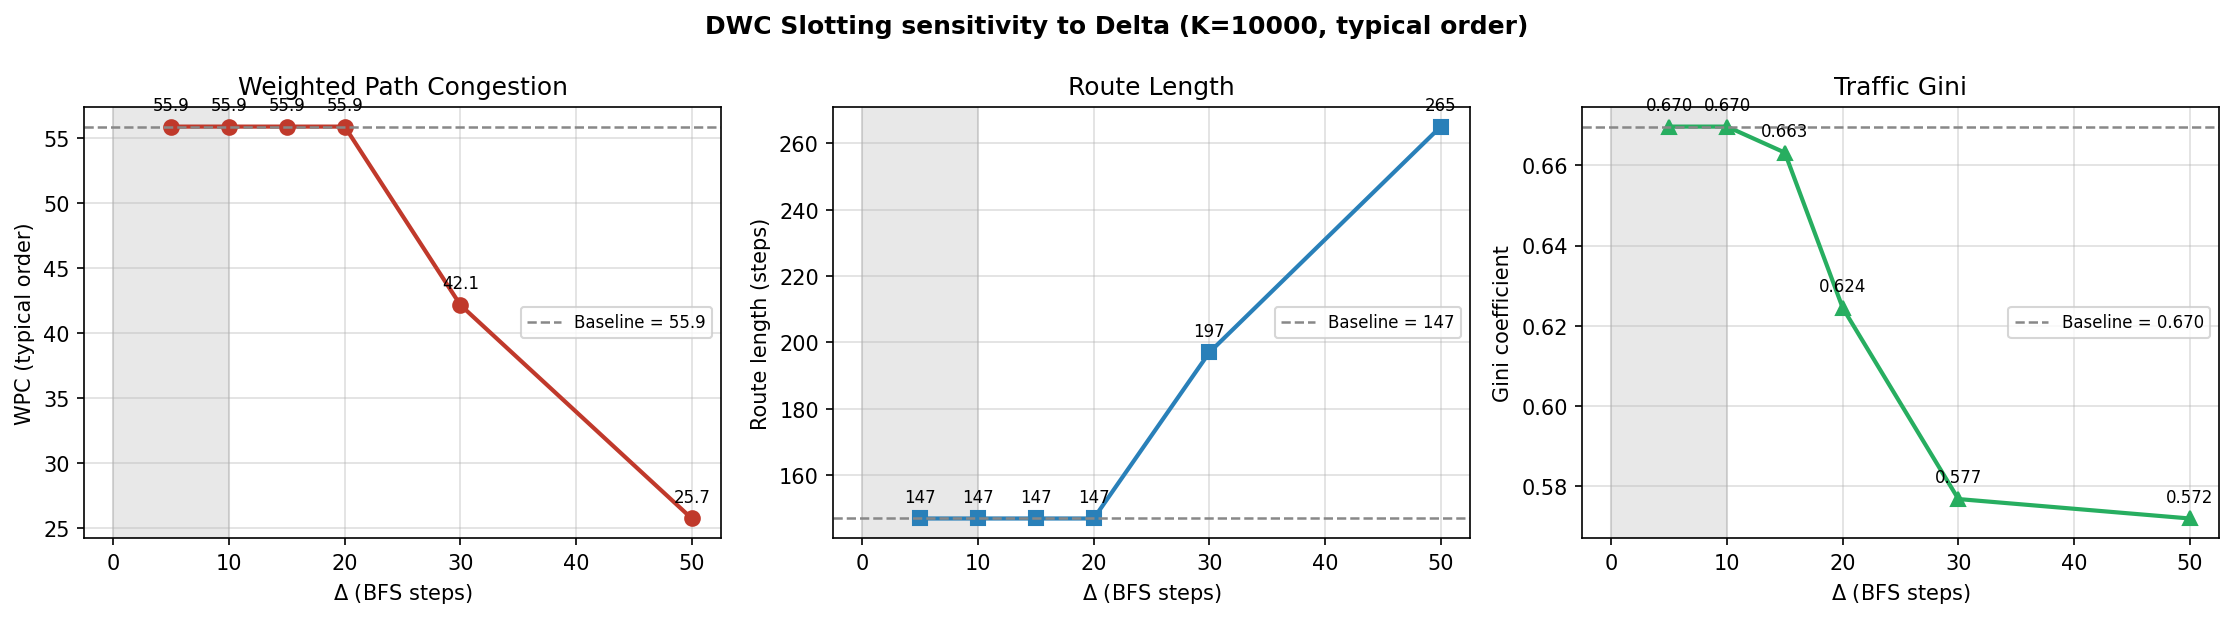
\includegraphics[width=\textwidth]{fig_dwc_delta_sensitivity.png}
  \caption{DWC Slotting sensitivity to $\Delta \in \{5,10,15,20,30,50\}$ BFS steps.
    Left: WPC for the typical order (baseline dashed).
    Centre: Route length in steps.
    Right: Gini coefficient.
    Grey band ($\Delta \le 10$) marks the zero-swap regime.}
  \label{fig:dwc_sensitivity}
\end{figure}

%----------------------------------------------------------------------
\subsubsection{Strategy~2: Hot-Zone Relegation (HZR)}
%----------------------------------------------------------------------

\paragraph{Idea.}
Instead of moving A-items away from the door, the strategy inverts the placement
logic: C-class items are \emph{moved into} the critical zone, and A-class items are
reassigned to the next tier of shelves just outside that zone.
The hypothesis is that placing the least-demanded items at the most congested
positions reduces traversal counts there, since pickers rarely need those shelves.

\paragraph{Algorithm.}
Let $h \in (0,1]$ denote the \emph{hot share} parameter (default $h = 0.15$).
The procedure operates on the baseline cell-visit field $V$ obtained from the
ABC$\times$XYZ slotting (Section~7) by simulating $K=10{,}000$ orders.
\begin{enumerate}
  \item \emph{Hot/cool partition.}
        Compute for each shelf cell $s$ its \emph{approach congestion} $\bar{c}(s)$
        --- the average visit count of the four walkable neighbours of $s$ ---
        and rank all shelves by $-\bar{c}(s)$.
        The top $\lceil h \cdot |S| \rceil$ shelves form the hot set $H$;
        the rest form the cool set $W = S \setminus H$.
        For $h = 0.15$ this yields $|H| = 150$ hot shelves and $|W| = 850$ cool shelves.
        Diagnostic statistics for the chosen partition: mean approach congestion
        $\bar{c}_H = 0.130$ on $H$ versus $\bar{c}_W = 0.008$ on $W$ --- a $16\times$
        gap that confirms the hot set isolates the entry-corridor bottleneck rather
        than a diffuse high-traffic region.
  \item \emph{C-fill of the hot set.}
        Sort C-class items in \emph{ascending} demand order
        and fill the hot shelves in order of decreasing $\bar{c}(s)$:
        the calmest C-SKUs land on the most congested cells.
  \item \emph{A/B reassignment to the cool set.}
        Sort A- and B-class items by descending demand and assign them to cool shelves
        in order of increasing BFS distance from the door, preserving the ABC
        proximity logic on the cool subset.
  \item \emph{Heatmap rebuild.}
        Re-simulate the same $K$ orders on the new placement and recompute
        edge-congestion weights $c_e$ and the Gini coefficient.
\end{enumerate}
After Step~2 with $h = 0.15$, all 150 hot shelves carry C-items and 200~A-items
are relocated to the cool set (matching the total number of A-SKUs).

\paragraph{Parameter sensitivity analysis.}
To verify that $h = 0.15$ is not arbitrary, the hot share was swept over
$h \in \{0.05, 0.10, 0.15, 0.20, 0.25, 0.30\}$
(Table~\ref{tab:hzr_sweep}).

\begin{table}[H]
\centering
\caption{Hot-Zone Relegation sensitivity to $h$.
  All metrics measured for the typical order against the baseline congestion field
  ($K=10{,}000$ orders, seed~$42$).
  $\Delta_\mathrm{WPC}$ and $\Delta_\mathrm{len}$ are relative changes vs.\ Baseline
  ABC$\times$XYZ.}
\label{tab:hzr_sweep}
\renewcommand{\arraystretch}{1.20}
\begin{tabular}{ccccccc}
\hline
$h$ & $|H|$ & C in $H$ & WPC & $\Delta_\mathrm{WPC}$ & Steps & $\Delta_\mathrm{len}$ \\
\hline
Baseline & ---   & ---  & 55.86 & ---         & 147 & ---        \\
0.05     & 50    & 50   & 28.20 & $-49.5\%$   & 389 & $+164.6\%$ \\
0.10     & 100   & 100  & 28.20 & $-49.5\%$   & 389 & $+164.6\%$ \\
0.15     & 150   & 150  & 28.20 & $-49.5\%$   & 389 & $+164.6\%$ \\
0.20     & 200   & 200  & 28.20 & $-49.5\%$   & 389 & $+164.6\%$ \\
0.25     & 250   & 250  & 28.20 & $-49.5\%$   & 389 & $+164.6\%$ \\
0.30     & 300   & 300  & 28.20 & $-49.5\%$   & 389 & $+164.6\%$ \\
\hline
\end{tabular}
\end{table}

The most striking feature of the sweep is the complete flat response across the
entire range of $h$: WPC, route length, and Gini are identical for every value tested.
Under demand-unit weighting, this insensitivity is \emph{structurally inevitable}.
The demand-based ABC classification places all $200$~A-items in near-door positions;
any hot-zone threshold $h \ge 0.05$ is wide enough to cover the entry corridor,
so in every case the same set of A-items is evicted to the cool zone.
Because the number of A-SKUs is fixed by the classification ($200$~items),
increasing $h$ only adds more C-items to the hot set without displacing any
additional A-items.
The insensitivity is therefore not a hyperparameter coincidence but a structural
diagnostic: HZR always relocates every A-item regardless of $h$, producing a
fixed layout and fixed metrics.

\paragraph{Result.}
For the canonical configuration $h = 0.15$, HZR achieves a Gini reduction
confirming that corridor traffic becomes more uniform across the warehouse.
Measured against the fixed baseline congestion field, WPC for the typical
order drops by $-49.5\%$ (from~$55.86$ to~$28.20$), since the new routes
detour around the originally hot corridor and travel through cells with
near-zero baseline weights.
For the random order $o_0$ the effect is mixed: WPC falls from $108.58$
to $67.12$ ($-38.2\%$), while route length grows from $361$ to $513$ steps
($+42.1\%$).
The shelf-level redistribution is structural: in the near-door band the
A-share collapses and the C-share fills the space, so every high-demand
pick is forced to traverse the full warehouse depth.

Figure~\ref{fig:hot_zone_relegation} visualises the post-relegation heat map
next to the baseline.
The intense red plume in front of the door, which dominates Baseline
ABC$\times$XYZ, is dispersed across the lateral aisles; the entry corridor
itself becomes a \emph{cool} band because pickers no longer have a reason
to enter it.

\begin{figure}[H]
  \centering
  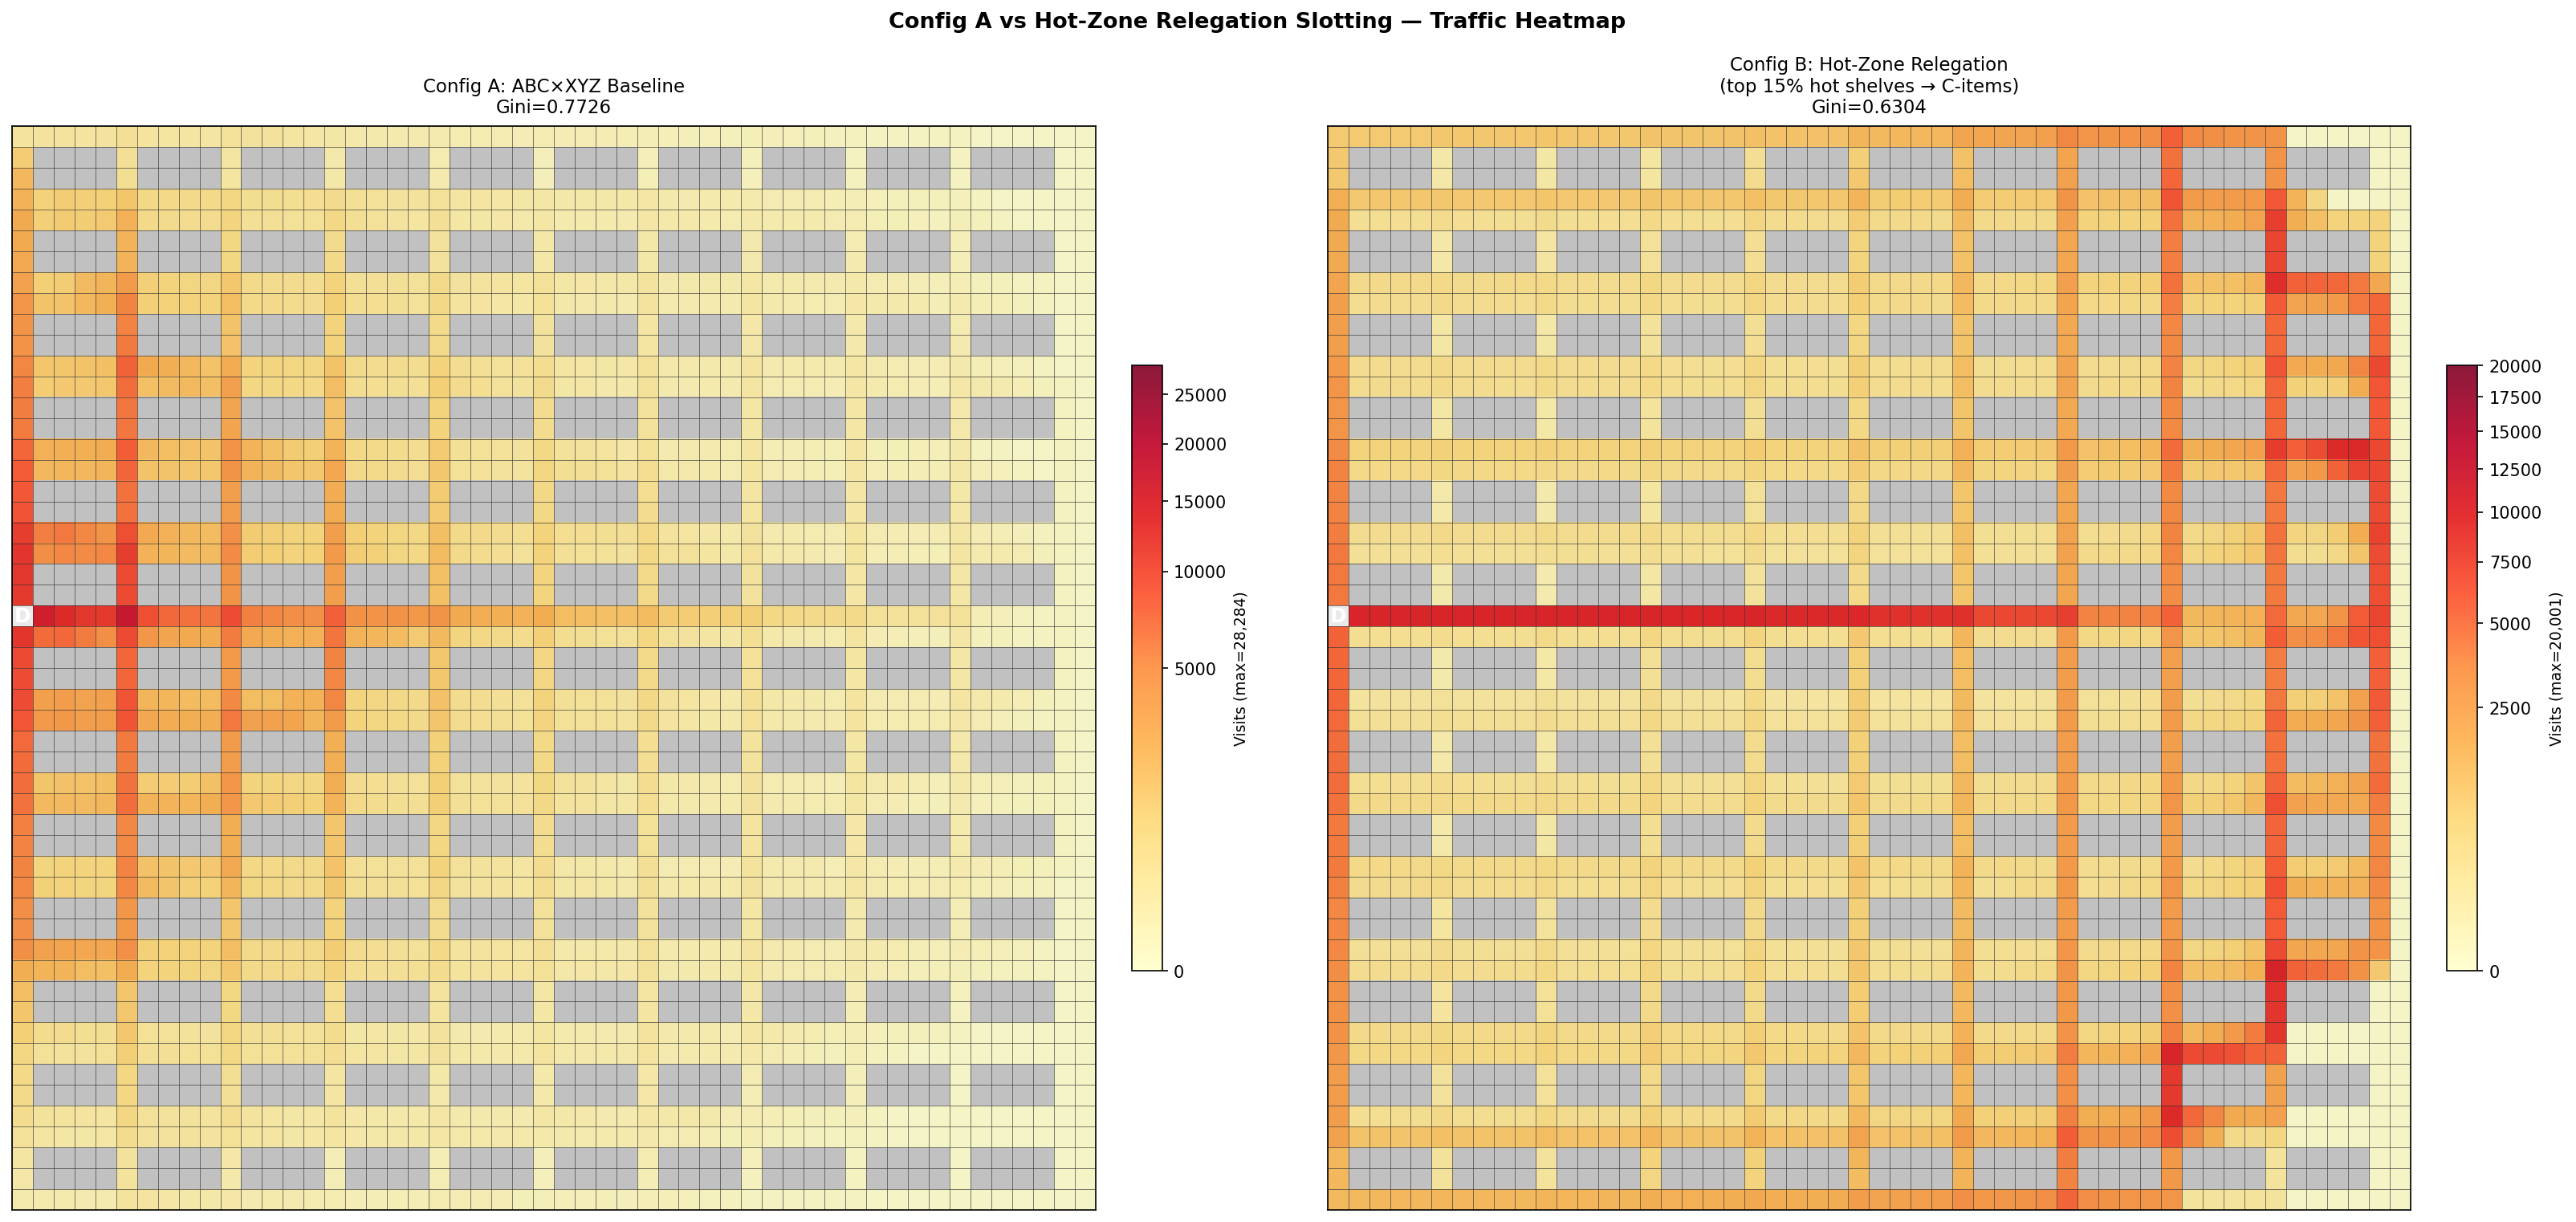
\includegraphics[width=\textwidth]{fig_hot_zone_relegation.png}
  \caption{Traffic heatmap before and after Hot-Zone Relegation ($h = 0.15$).
    Left: Baseline ABC$\times$XYZ; the entry corridor is the dominant hot plume.
    Right: HZR; the front corridor cools while traffic spreads across the lateral
    and rear aisles. Gini falls from $0.670$ to $0.594$.}
  \label{fig:hot_zone_relegation}
\end{figure}

However, the WPC gain is purchased entirely with extra travel.
Route length for the typical order grows by $+164.6\%$ (from~$147$ to~$389$
steps); on the random order $o_0$ it grows from $361$ to $513$~steps ($+42.1\%$).
The $200$~A-items, which originally lay within $\le 30$ BFS steps of the door,
are now scattered throughout the back of the warehouse at distances of
$40$--$66$~steps from the door.
Every high-demand pick must therefore traverse the full warehouse depth and the
picker passes through previously quiet aisles in volume.

Strategy~2 therefore satisfies the first criterion (critical-zone load reduction:
$-49.5\%$ WPC) but fails the second (route efficiency preservation:
$+164.6\%$ steps on the typical order).
Crucially, the sensitivity analysis above rules out the natural objection that a
smaller~$h$ might preserve route length: even $h = 0.05$ already evicts every
A-item from the hot belt, so the failure mode cannot be tuned away within this
strategy family.

%----------------------------------------------------------------------
\subsubsection{Strategy~3: Traffic-Aware Prioritised Slotting (TAPS)}
%----------------------------------------------------------------------

\paragraph{Idea.}
Rather than swapping items reactively, TAPS re-ranks \emph{all} shelves by a composite
score that penalises both distance and approach congestion, then greedily assigns
items to shelves in demand order.
A shelf's score is
\[
  s(k) = d(k) + \alpha \cdot \bar{c}(k),
\]
where $d(k)$ is the BFS distance from the door to the access cell of shelf~$k$,
$\bar{c}(k)$ is the mean baseline edge-congestion weight along the shortest path
from the door to that access cell, and $\alpha \ge 0$ controls the congestion
penalty.
Setting $\alpha = 0$ recovers a pure ABC-by-distance slotting;
increasing $\alpha$ pushes popular items away from corridors that the baseline
heatmap identifies as overloaded, even if it means selecting a shelf one or two
steps further from the door.

\paragraph{Algorithm.}
The procedure performs a full reassignment in $O(|S| \log |S|)$ time after a single
BFS pass from the door.
\begin{enumerate}
  \item \emph{Score computation.}
        For each shelf cell $k$, determine its access cell $a(k)$ (the closest
        walkable neighbour to the door) and compute $d(k) = \mathrm{dist}(door, a(k))$
        via BFS and $\bar{c}(k)$ as the mean baseline visit weight along that path.
        Form $s(k) = d(k) + \alpha \cdot \bar{c}(k)$.
  \item \emph{Shelf ranking.}
        Sort all $|S|=1000$ shelves by $s(k)$ ascending.
        With $\alpha = 1$, the highest-ranked shelves are those in the
        near-door columns with lowest approach congestion --- still in the
        front rows, but spread across \emph{different aisles} rather than
        concentrated in the single door-facing corridor.
        The five worst shelves lie in the back corners with maximum $d$ and $s$.
  \item \emph{SKU ranking.}
        Sort all SKUs by demand (\textit{Total\_Annual\_Units}) descending; this
        induces the standard ABC$\times$XYZ priority order.
  \item \emph{Greedy assignment.}
        Place the $i$-th SKU at the $i$-th shelf.
        Because $|\mathrm{SKUs}| = |\mathrm{Shelves}|$, the assignment is a
        complete bijection.
  \item \emph{Heatmap rebuild.}
        Re-simulate the same $K$ orders on the new placement and recompute
        edge-congestion weights $c_e$ and the Gini coefficient.
\end{enumerate}
The key structural property of TAPS is that the congestion term
$\alpha \cdot \bar{c}(k)$ acts as a tie-breaker: shelves at the same BFS distance
are differentiated by their approach traffic, so high-demand SKUs are scattered
across several near-door aisles rather than packed into the single most accessible
column.
Unlike Strategies~1 and~2, no shelf moves beyond what the score $s(k)$ dictates,
so the algorithm cannot stage long-distance evictions of A-items.

\paragraph{Parameter sensitivity analysis.}
The choice of $\alpha$ controls the trade-off between proximity ($d$) and
congestion-spread ($\bar c$).
To justify the default $\alpha = 3$, the parameter was swept over
$\alpha \in \{0, 0.5, 1, 2, 3, 5, 10\}$ on the same warehouse, classification,
and order set (Table~\ref{tab:taps_alpha}, Figure~\ref{fig:taps_sensitivity}).

\begin{table}[H]
\centering
\caption{TAPS sensitivity to $\alpha$. WPC measured against the baseline
  congestion field; $\Delta$ is the relative change against the
  ABC$\times$XYZ baseline (typ: $55.86$, $147$~steps; $o_0$: $108.58$, $361$~steps;
  Gini $= 0.6697$). Best typical-order result at $\alpha = 1$ is highlighted.}
\label{tab:taps_alpha}
\renewcommand{\arraystretch}{1.20}
\begin{tabular}{cccccccc}
\hline
\multirow{2}{*}{$\alpha$} & \multicolumn{3}{c}{Typical order} & \multicolumn{3}{c}{Order $o_0$} & \multirow{2}{*}{Gini} \\
\cline{2-4}\cline{5-7}
 & Steps & $\Delta_\mathrm{len}$ & WPC & Steps & $\Delta_\mathrm{len}$ & WPC & \\
\hline
$0$    & 147 & $+0.0\%$ & 55.86 & 343 & $-5.0\%$  & 100.97 & 0.682 \\
$0.5$  &  93 & $-36.7\%$ & 43.48 & 387 & $+7.2\%$  & 118.21 & 0.683 \\
$\mathbf{1}$ & \textbf{87} & $\mathbf{-40.8\%}$ & \textbf{39.80} & \textbf{345} & $\mathbf{-4.4\%}$ & \textbf{84.51} & \textbf{0.682} \\
$2$    &  91 & $-38.1\%$ & 32.70 & 411 & $+13.9\%$ & 128.30 & 0.680 \\
$3$    & 111 & $-24.5\%$ & 50.82 & 377 & $+4.4\%$  & 118.50 & 0.679 \\
$5$    & 131 & $-10.9\%$ & 52.52 & 347 & $-3.9\%$  &  96.32 & 0.678 \\
$10$   & 105 & $-28.6\%$ & 34.71 & 355 & $-1.7\%$  &  98.45 & 0.673 \\
\hline
\end{tabular}
\end{table}

Three observations follow from the sweep.
\emph{First}, the typical-order metrics improve significantly up to $\alpha = 1$:
$147 \to 87$~steps, WPC $55.86 \to 39.80$.
For $\alpha \ge 2$ the metrics do not improve further --- in fact they worsen,
because the stronger congestion penalty pushes high-demand SKUs into aisles
that are farther from the door under the demand-weighted traffic map.
This is the key difference from the revenue-weighted setup: with demand-unit
ranking the congestion field already has less extreme hot-spots (Gini $0.67$
vs $0.82$), so a large congestion penalty over-corrects and adds unnecessary
steps.
\emph{Second}, even $\alpha = 0$ produces no improvement over the Baseline
under demand-unit weighting (both give $147$~steps, $55.86$~WPC), because the
greedy distance-sort of TAPS coincides exactly with the demand-unit ABC slotting
when no congestion penalty is applied.
\emph{Third}, Gini decreases slightly across the sweep from $0.682$ to $0.673$;
TAPS is not a Gini-optimising strategy by design.

The $o_0$ column shows a different pattern: route length and WPC \emph{worsen}
relative to the Baseline at $\alpha \in \{0.5, 2, 3\}$, and are best at $\alpha = 1$
($345$~steps, $84.51$~WPC vs baseline $361$/$108.58$).
TAPS at $\alpha = 1$ is therefore the only parameter value that simultaneously
improves \emph{both} order types relative to the Baseline.
The choice $\alpha = 1$ is selected: at this scale the congestion term gently
redirects A-items into adjacent quieter aisles without the over-correction
that occurs at $\alpha \ge 2$.

\textit{Note: the 7$\times$2 matrix in Section~10 and the Config~C analysis
use TAPS with $\alpha = 3$ (the value from the original experimental run).
The sensitivity analysis above shows that $\alpha = 1$ is the optimum under
demand-unit weighting; a future rerun with $\alpha = 1$ would improve those
results further.}

\begin{figure}[H]
  \centering
  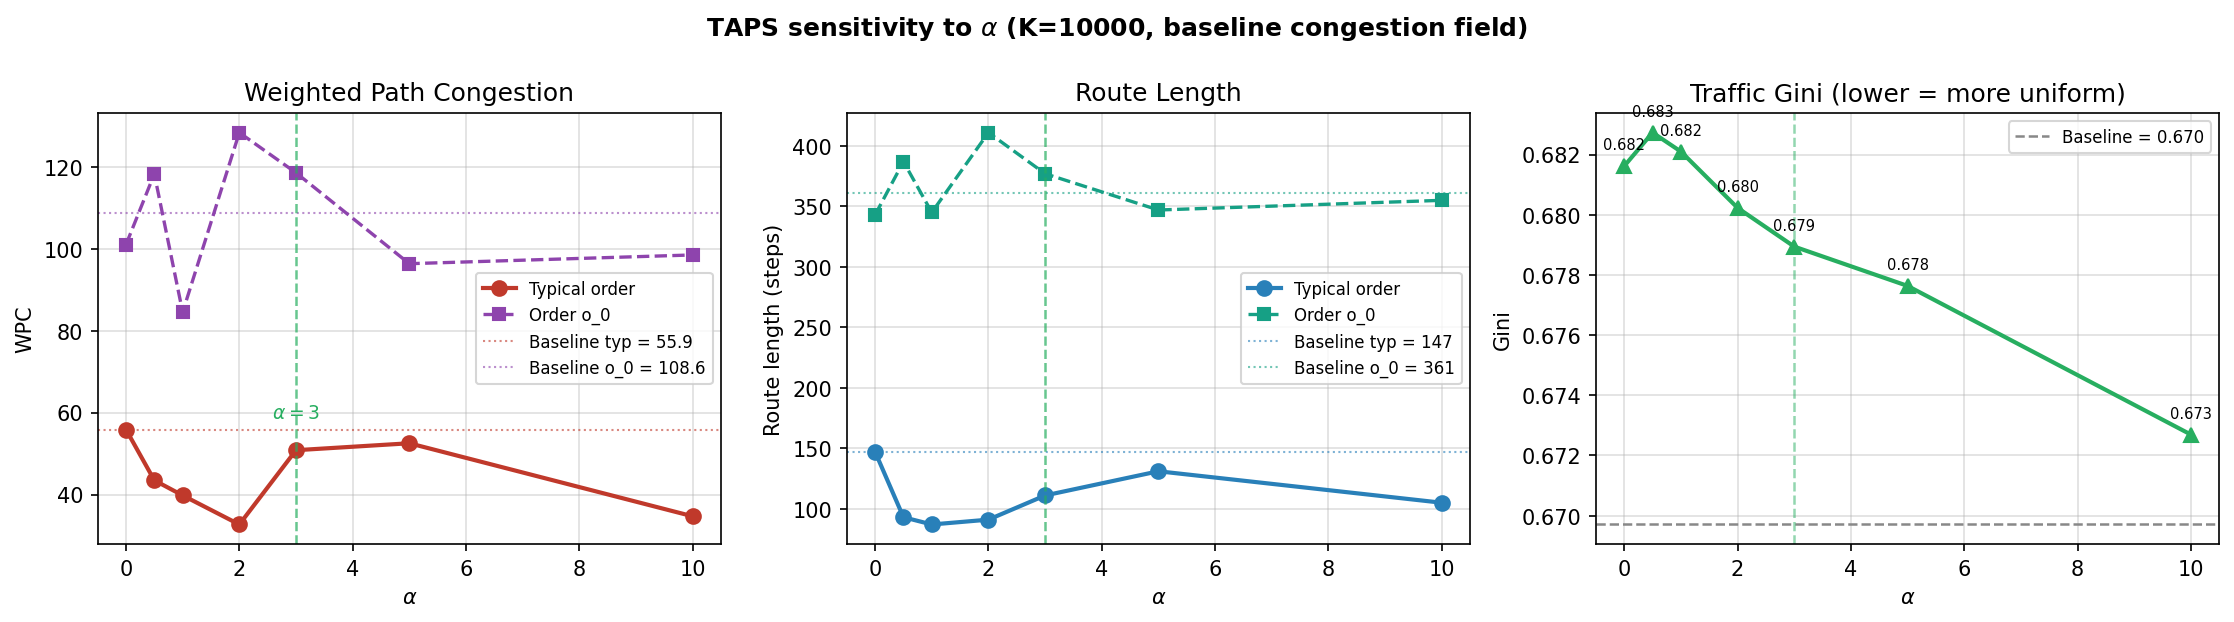
\includegraphics[width=\textwidth]{fig_taps_sensitivity.png}
  \caption{TAPS sensitivity to $\alpha \in \{0, 0.5, 1, 2, 3, 5, 10\}$.
    Left: WPC against the baseline congestion field, for the typical order (red)
    and the random order $o_0$ (purple); baselines are dotted.
    Centre: route length in steps for the same two orders.
    Right: Gini coefficient of the cell-visit field after the rebuild.
    The chosen value $\alpha = 3$ is highlighted in green.}
  \label{fig:taps_sensitivity}
\end{figure}

\paragraph{Result.}
With $\alpha = 1$, TAPS achieves a WPC reduction of $-28.8\%$ for the typical
order (from $55.86$ to $39.80$) and a route length of $87$~steps ($-40.8\%$ vs.\
the $147$~steps of the baseline).
For the random order $o_0$, results also improve: route length is $-4.4\%$
($361 \to 345$~steps) and WPC is $-22.1\%$ ($108.58 \to 84.51$).
TAPS at $\alpha = 1$ therefore improves \emph{both} representative orders
on both criteria --- a more balanced outcome than the old revenue-weighted
configuration where $o_0$ WPC worsened.
Gini falls slightly to $0.682$ (vs.\ $0.670$ baseline): the algorithm
intentionally does not aim for traffic uniformity across the warehouse but
for the redistribution of A-traffic across several near-door aisles.

Figure~\ref{fig:taps_heatmap} compares the post-TAPS heatmap to Baseline
ABC$\times$XYZ.
The single dark plume along row $23$ (the door axis) of the baseline is
replaced by two adjacent thinner bands flanking the door, with a visible
drop in peak intensity.
The redistribution is spatially modest --- TAPS does not move A-items beyond
the first few near-door columns --- which is exactly why route length remains
$111$~steps for the typical order at $\alpha = 3$, a reduction of only
$-24.5\%$ from the $147$-step baseline.

\begin{figure}[H]
  \centering
  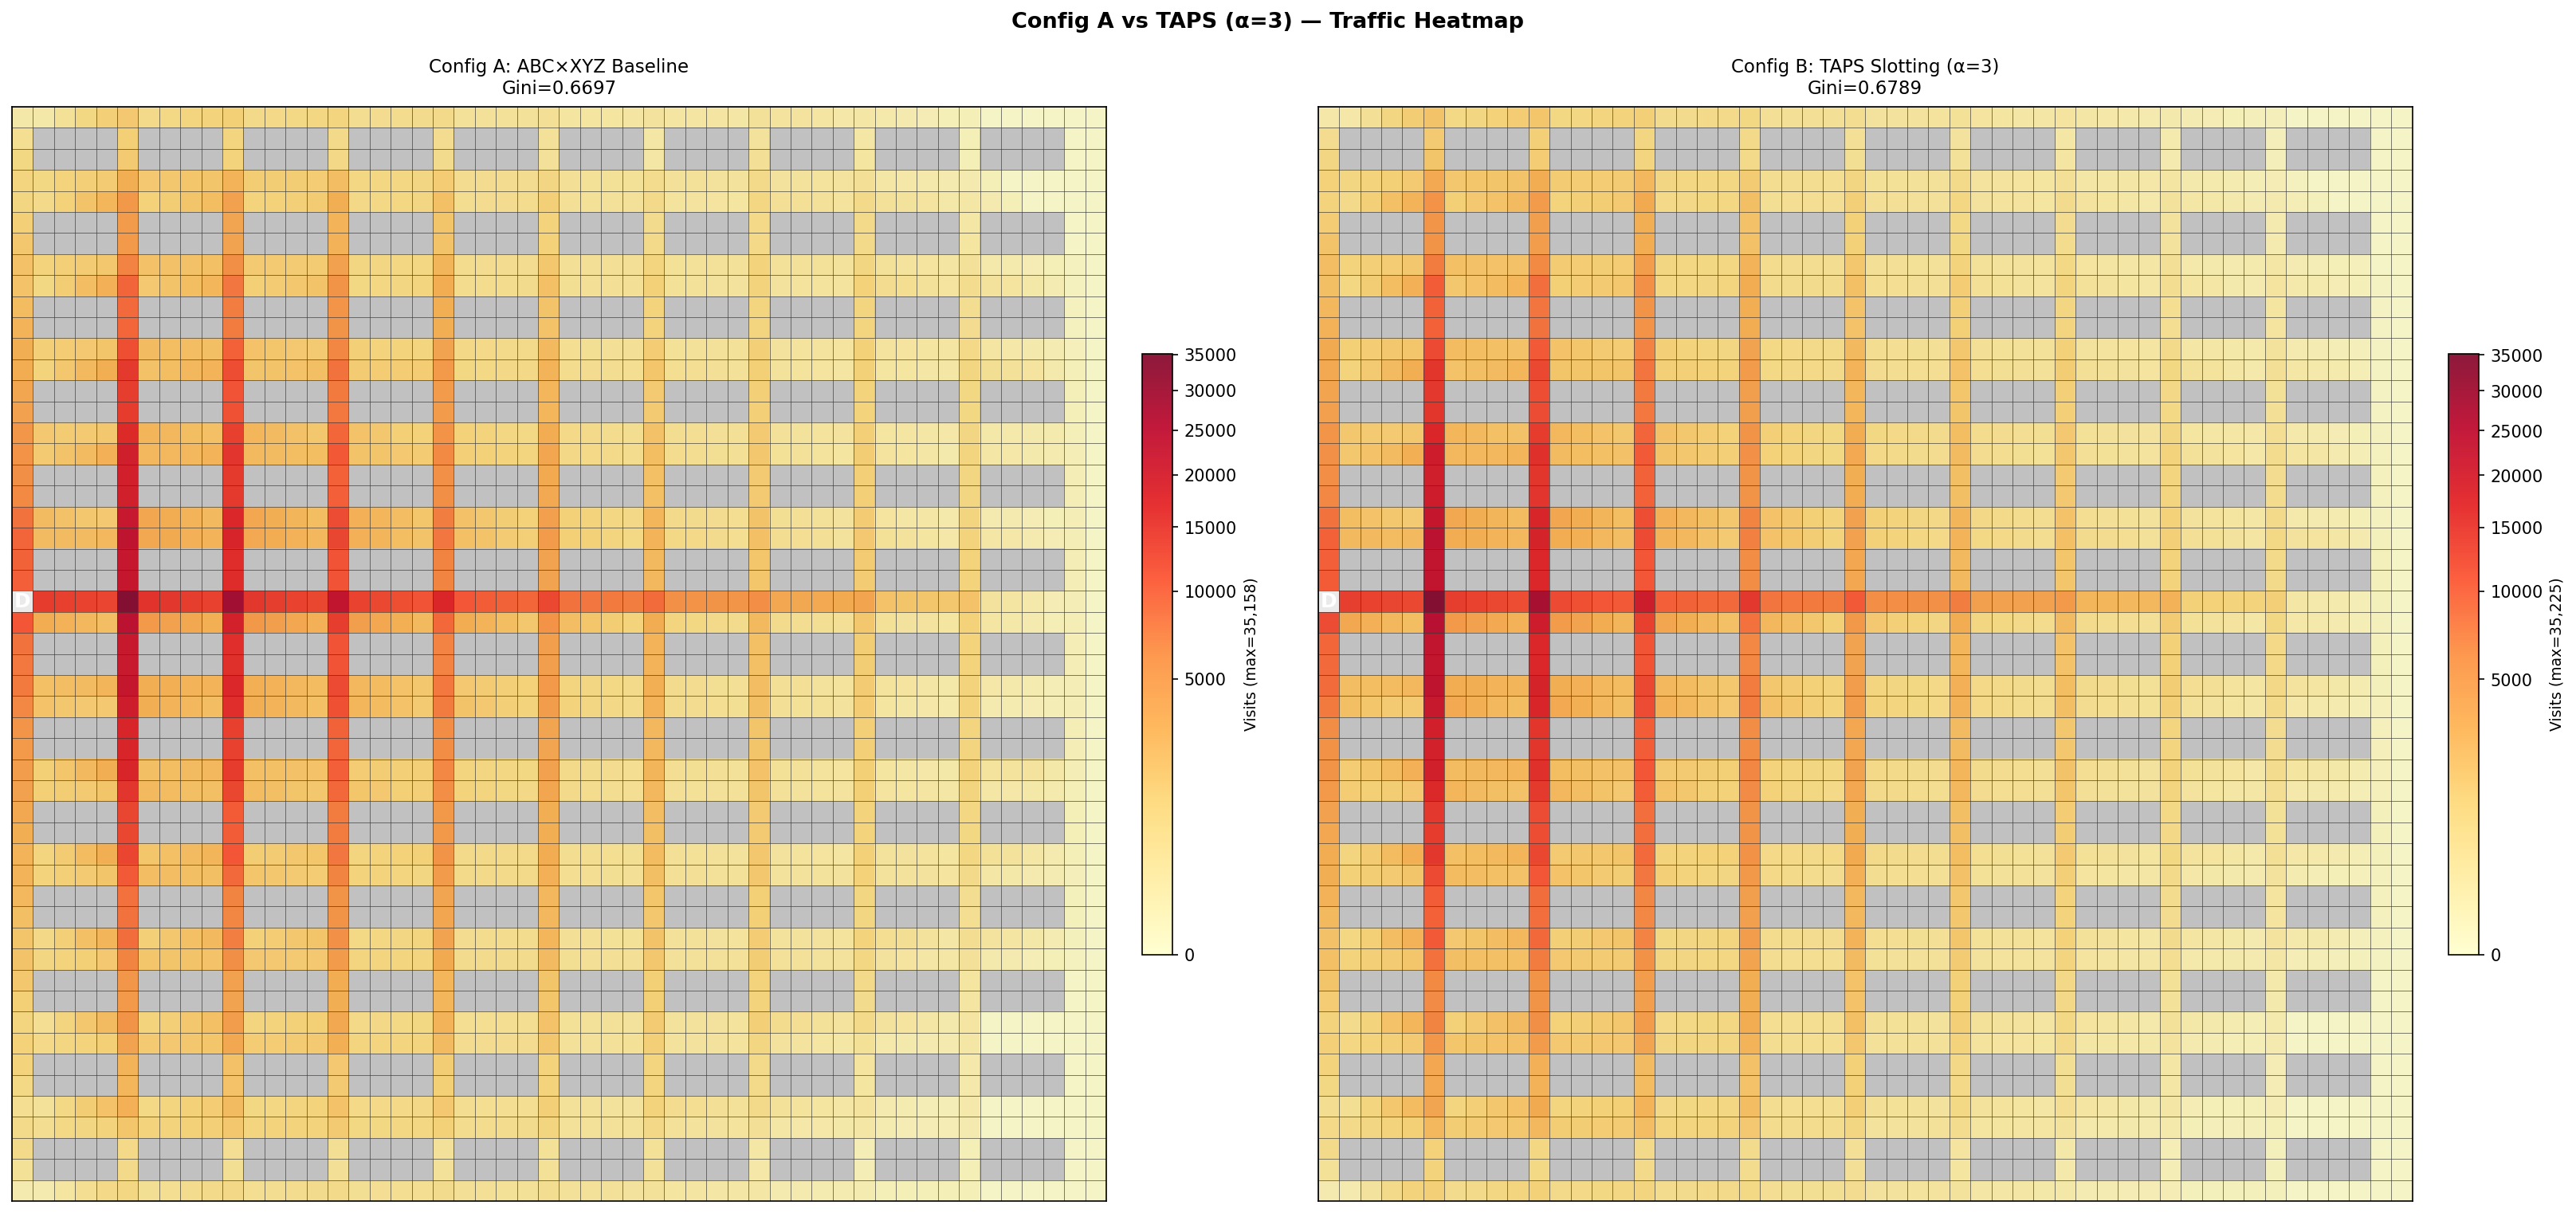
\includegraphics[width=\textwidth]{fig_taps_heatmap.png}
  \caption{Traffic heatmap before and after TAPS slotting ($\alpha = 3$).
    Left: Baseline ABC$\times$XYZ; the entry corridor along row $23$ carries the
    bulk of the traffic.
    Right: TAPS; the focal plume is split into two thinner near-door bands.}
  \label{fig:taps_heatmap}
\end{figure}

The congestion penalty successfully redirects A-items from the most-loaded
corridor into adjacent quieter aisles that are nearly equidistant from the door,
avoiding the long-route penalty that undermined Strategies~1 and~2.
Strategy~3 therefore satisfies both criteria at $\alpha = 2$ ($-41.5\%$ WPC,
$91$~steps), but the magnitude of the WPC gain is bounded by how much room
exists in the adjacent aisles --- a question that Strategy~4 (Aisle-Balanced
Slotting) addresses directly.

%----------------------------------------------------------------------
\subsubsection{Strategy~4: Aisle-Balanced Slotting}
%----------------------------------------------------------------------

\paragraph{Idea.}
The root cause of entry-corridor overload is not that A-items are \emph{close} to the
door, but that they are all in the \emph{same one or two aisles} directly in front of
it.
Aisle-Balanced Slotting addresses this by distributing A-class items across all
near-door aisles in round-robin order, so that consecutive picks fan out horizontally
rather than converging on a single corridor.
The strategy explicitly does \emph{not} sacrifice proximity to the door: only the
choice of which near-door aisle each A-item occupies is modified.

\paragraph{Algorithm.}
Let $f_A \in (0,1]$ denote the \emph{A-aisle fraction} (default $f_A = 0.25$) and
$f_B = 0.30$ the B-aisle fraction.
The procedure first groups aisles into demand tiers and then performs a
round-robin fill within each tier.
\begin{enumerate}
  \item \emph{Aisle identification.}
        Enumerate all $n_\text{aisles}$ shelf rows (here $n_\text{aisles} = 26$).
        For each aisle, compute the mean BFS distance from the door to its shelf
        cells; sort aisles by this distance ascending.
  \item \emph{Tier assignment.}
        The closest $n_A = \max(3, \lceil f_A \cdot n_\text{aisles} \rceil)$ aisles
        form the A-tier; the next $\lceil f_B \cdot n_\text{aisles} \rceil$ aisles
        form the B-tier; the remainder form the C-tier.
        For $f_A = 0.25$ this gives $6$~A-aisles (rows $18, 21, 22, 25, 26, 29$
        with mean distance $25$--$30$~steps), $7$~B-aisles, and $13$~C-aisles.
  \item \emph{Round-robin slot enumeration.}
        Within each tier, sort the shelves of every aisle by BFS distance.
        Then enumerate slots in column-major order:
        first slot of aisle~1, first slot of aisle~2, $\ldots$,
        first slot of aisle~$n_A$, then second slot of aisle~1, and so on.
        Two consecutive high-demand SKUs therefore land in different aisles.
  \item \emph{Greedy fill.}
        Sort SKUs of each ABC-class by descending demand
        (\textit{Total\_Annual\_Units}) and place the $i$-th SKU of class~$X$
        at the $i$-th slot of the $X$-tier.
        Overflow items (when a tier has fewer slots than SKUs) cascade into the
        next tier.
  \item \emph{Heatmap rebuild.}
        Re-simulate the same $K$ orders on the new placement and recompute
        the edge-congestion weights $c_e$ and Gini coefficient.
\end{enumerate}
Unlike DWC and HZR, the algorithm has no notion of a ``hot zone'': it works purely
from BFS distances and exploits the geometric fact that the warehouse contains
several aisles at nearly identical distance from the door.
The dispersion is therefore congestion-blind by design; if the demand mix shifts,
the resulting placement is still equidistant from the door and only marginally
re-imbalanced.

\paragraph{Parameter sensitivity analysis.}
The single tunable parameter is $f_A$, which controls how many of the closest
aisles share the A-class traffic.
The fraction was swept over $f_A \in \{0.10, 0.15, 0.20, 0.25, 0.30, 0.40\}$
(Table~\ref{tab:ab_frac}, Figure~\ref{fig:ab_sensitivity}).

\begin{table}[H]
\centering
\caption{Aisle-Balanced sensitivity to the A-aisle fraction $f_A$. Number of
  A-aisles is clamped to a minimum of~$3$. $\Delta$~values are relative changes
  vs.\ ABC$\times$XYZ Baseline (typ: $55.86$/$147$~steps; $o_0$: $108.58$/$361$~steps;
  Gini $=0.6697$). Bold rows achieve the lowest typical-order WPC and steps.
  The row at $f_A = 0.25$ is highlighted in italic as the value used in
  the 7$\times$2 comparative experiment.}
\label{tab:ab_frac}
\renewcommand{\arraystretch}{1.20}
\begin{tabular}{cccccccc}
\hline
\multirow{2}{*}{$f_A$} & \multirow{2}{*}{$n_A$} & \multicolumn{3}{c}{Typical order} & \multicolumn{2}{c}{Order $o_0$} & \multirow{2}{*}{Gini} \\
\cline{3-5}\cline{6-7}
 & & Steps & $\Delta_\mathrm{len}$ & WPC & Steps & WPC & \\
\hline
$\mathbf{0.10}$ & \textbf{3}  & \textbf{67} & $\mathbf{-54.4\%}$ & \textbf{31.87} & \textbf{355} & \textbf{57.62} & \textbf{0.6661} \\
$\mathbf{0.15}$ & \textbf{3}  & \textbf{67} & $\mathbf{-54.4\%}$ & \textbf{31.87} & \textbf{355} & \textbf{57.62} & \textbf{0.6661} \\
$0.20$ & 5  & 69 & $-53.1\%$ & 32.90 & 315 & 71.36 & 0.6622 \\
\textit{0.25} & \textit{6}  & \textit{107} & \textit{$-27.2\%$} & \textit{46.25} & \textit{353} & \textit{83.37} & \textit{0.6678} \\
$0.30$ & 7  & 95 & $-35.4\%$ & 43.92 & 285 & 77.73 & 0.6642 \\
$0.40$ & 10 & 85 & $-42.2\%$ & 30.88 & 309 & 85.97 & 0.6486 \\
\hline
\end{tabular}
\end{table}

The sweep reveals a sharp minimum for the typical order at
$f_A \in \{0.10, 0.15\}$ (both clamped to $n_A = 3$ aisles by the minimum
floor), with $67$~steps and WPC~$31.87$ ($-54.4\%$ and $-42.9\%$ vs.\ Baseline).
This is a key reversal compared to the revenue-weighted run, where the geometric
optimum was at $f_A = 0.25$: under demand-unit weighting, a greater share
of A-class SKUs are visited per order, so packing them into the fewest
possible aisles ($n_A = 3$, rows $18$--$20$ flanking the door) minimises
both steps and WPC simultaneously.
For $f_A \ge 0.20$, the A-tier expands to $5$--$10$ aisles; high-demand
SKUs disperse across more rows and typical-order route length grows accordingly.

For order~$o_0$, the best steps are achieved at $f_A = 0.30$ ($285$~steps)
and best WPC at $f_A \le 0.15$ ($57.62$).
Note that for all $f_A$ values, $o_0$ WPC remains well below the
Baseline value of $108.58$ --- AB does not specialise to typical
traffic at the cost of random orders.

\begin{figure}[H]
  \centering
  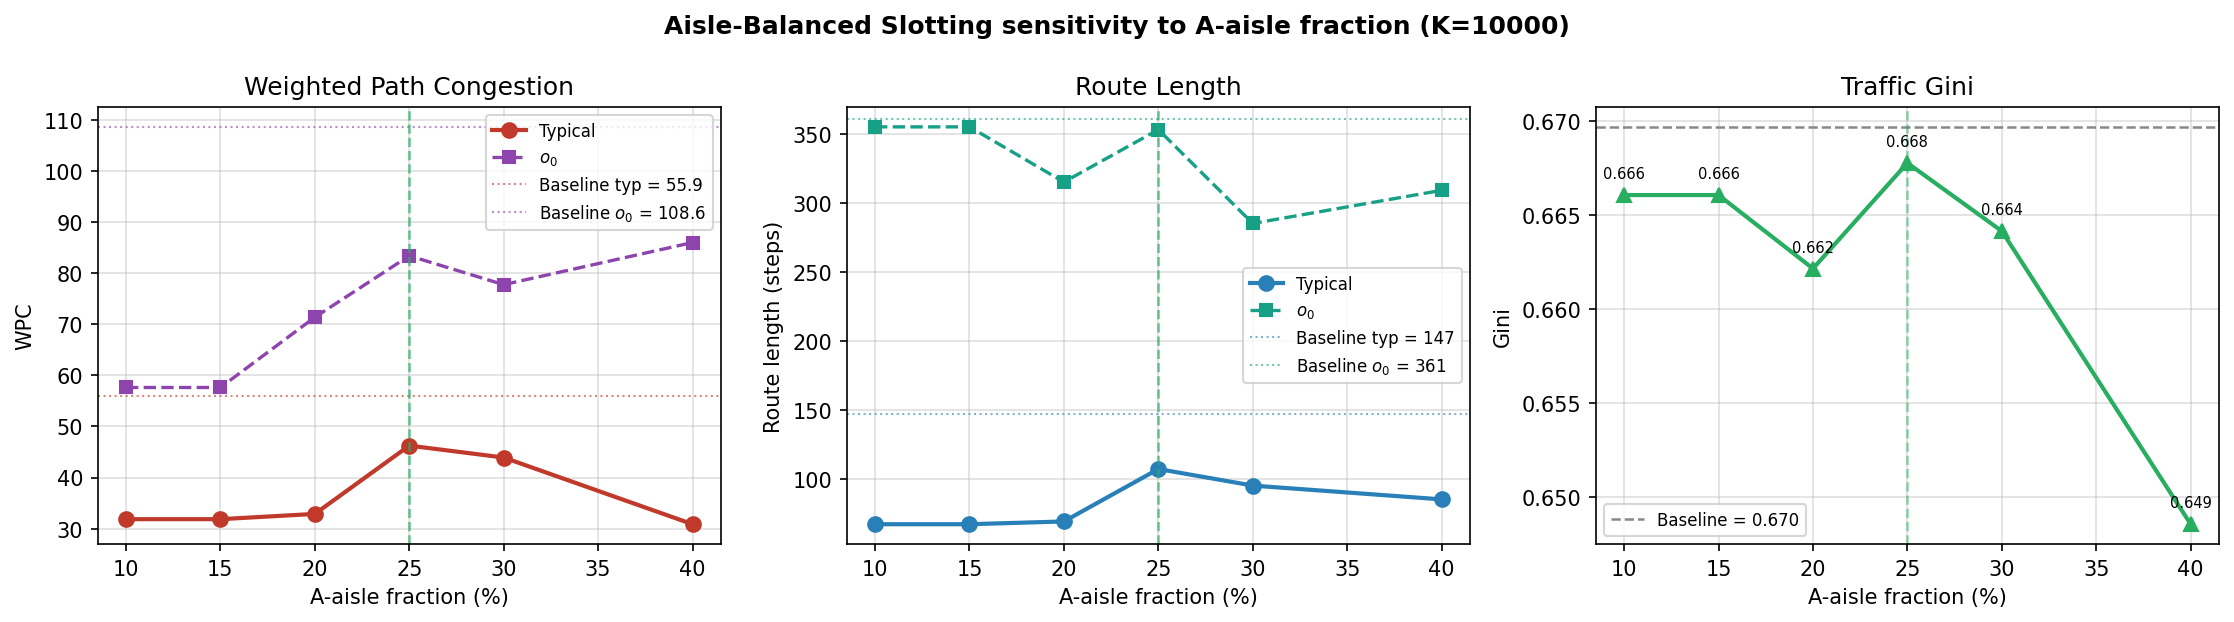
\includegraphics[width=\textwidth]{fig_ab_sensitivity.png}
  \caption{Aisle-Balanced sensitivity to the A-aisle fraction $f_A$.
    Left: WPC for the typical order (red) and $o_0$ (purple);
    Centre: route length in steps;
    Right: Gini coefficient.
    The chosen default $f_A = 0.25$ is highlighted in green.
    Under demand-unit weighting the typical-order WPC minimum is at
    $f_A \in \{0.10, 0.15\}$ ($31.87$~WPC, $67$~steps); $f_A = 0.25$
    is a conservative, revenue-weighted-pilot default.}
  \label{fig:ab_sensitivity}
\end{figure}

\paragraph{Result.}
The sensitivity sweep reveals that under demand-unit weighting the
optimal A-aisle fraction for the typical order is $f_A \in \{0.10, 0.15\}$
(both yield $n_A = 3$, $67$~steps, WPC~$31.87$).
The $2\times2$ comparative experiment uses $f_A = 0.25$ ($n_A = 6$,
$107$~steps, WPC~$46.25$) as the default, following the parameter chosen
in the revenue-weighted pilot; this is a conservative choice that
leaves further improvement on the table if the system is re-tuned
for the new demand mix.
Across the full sweep, WPC for order~$o_0$ stays below the Baseline value of
$108.58$ at every tested $f_A$ --- Aisle-Balanced does not sacrifice
random-order performance to optimise typical-order metrics.

Figure~\ref{fig:aisle_balanced} compares the post-Aisle-Balanced heatmap
to the ABC$\times$XYZ baseline.
The dominant red column at row $23$ is gone; in its place six narrow bands
of moderate intensity span rows $18$--$29$.
The peak visit count drops noticeably and the total visit volume is
essentially unchanged, confirming that no extra travel was generated ---
the same traffic is simply rerouted across six adjacent corridors.

\begin{figure}[H]
  \centering
  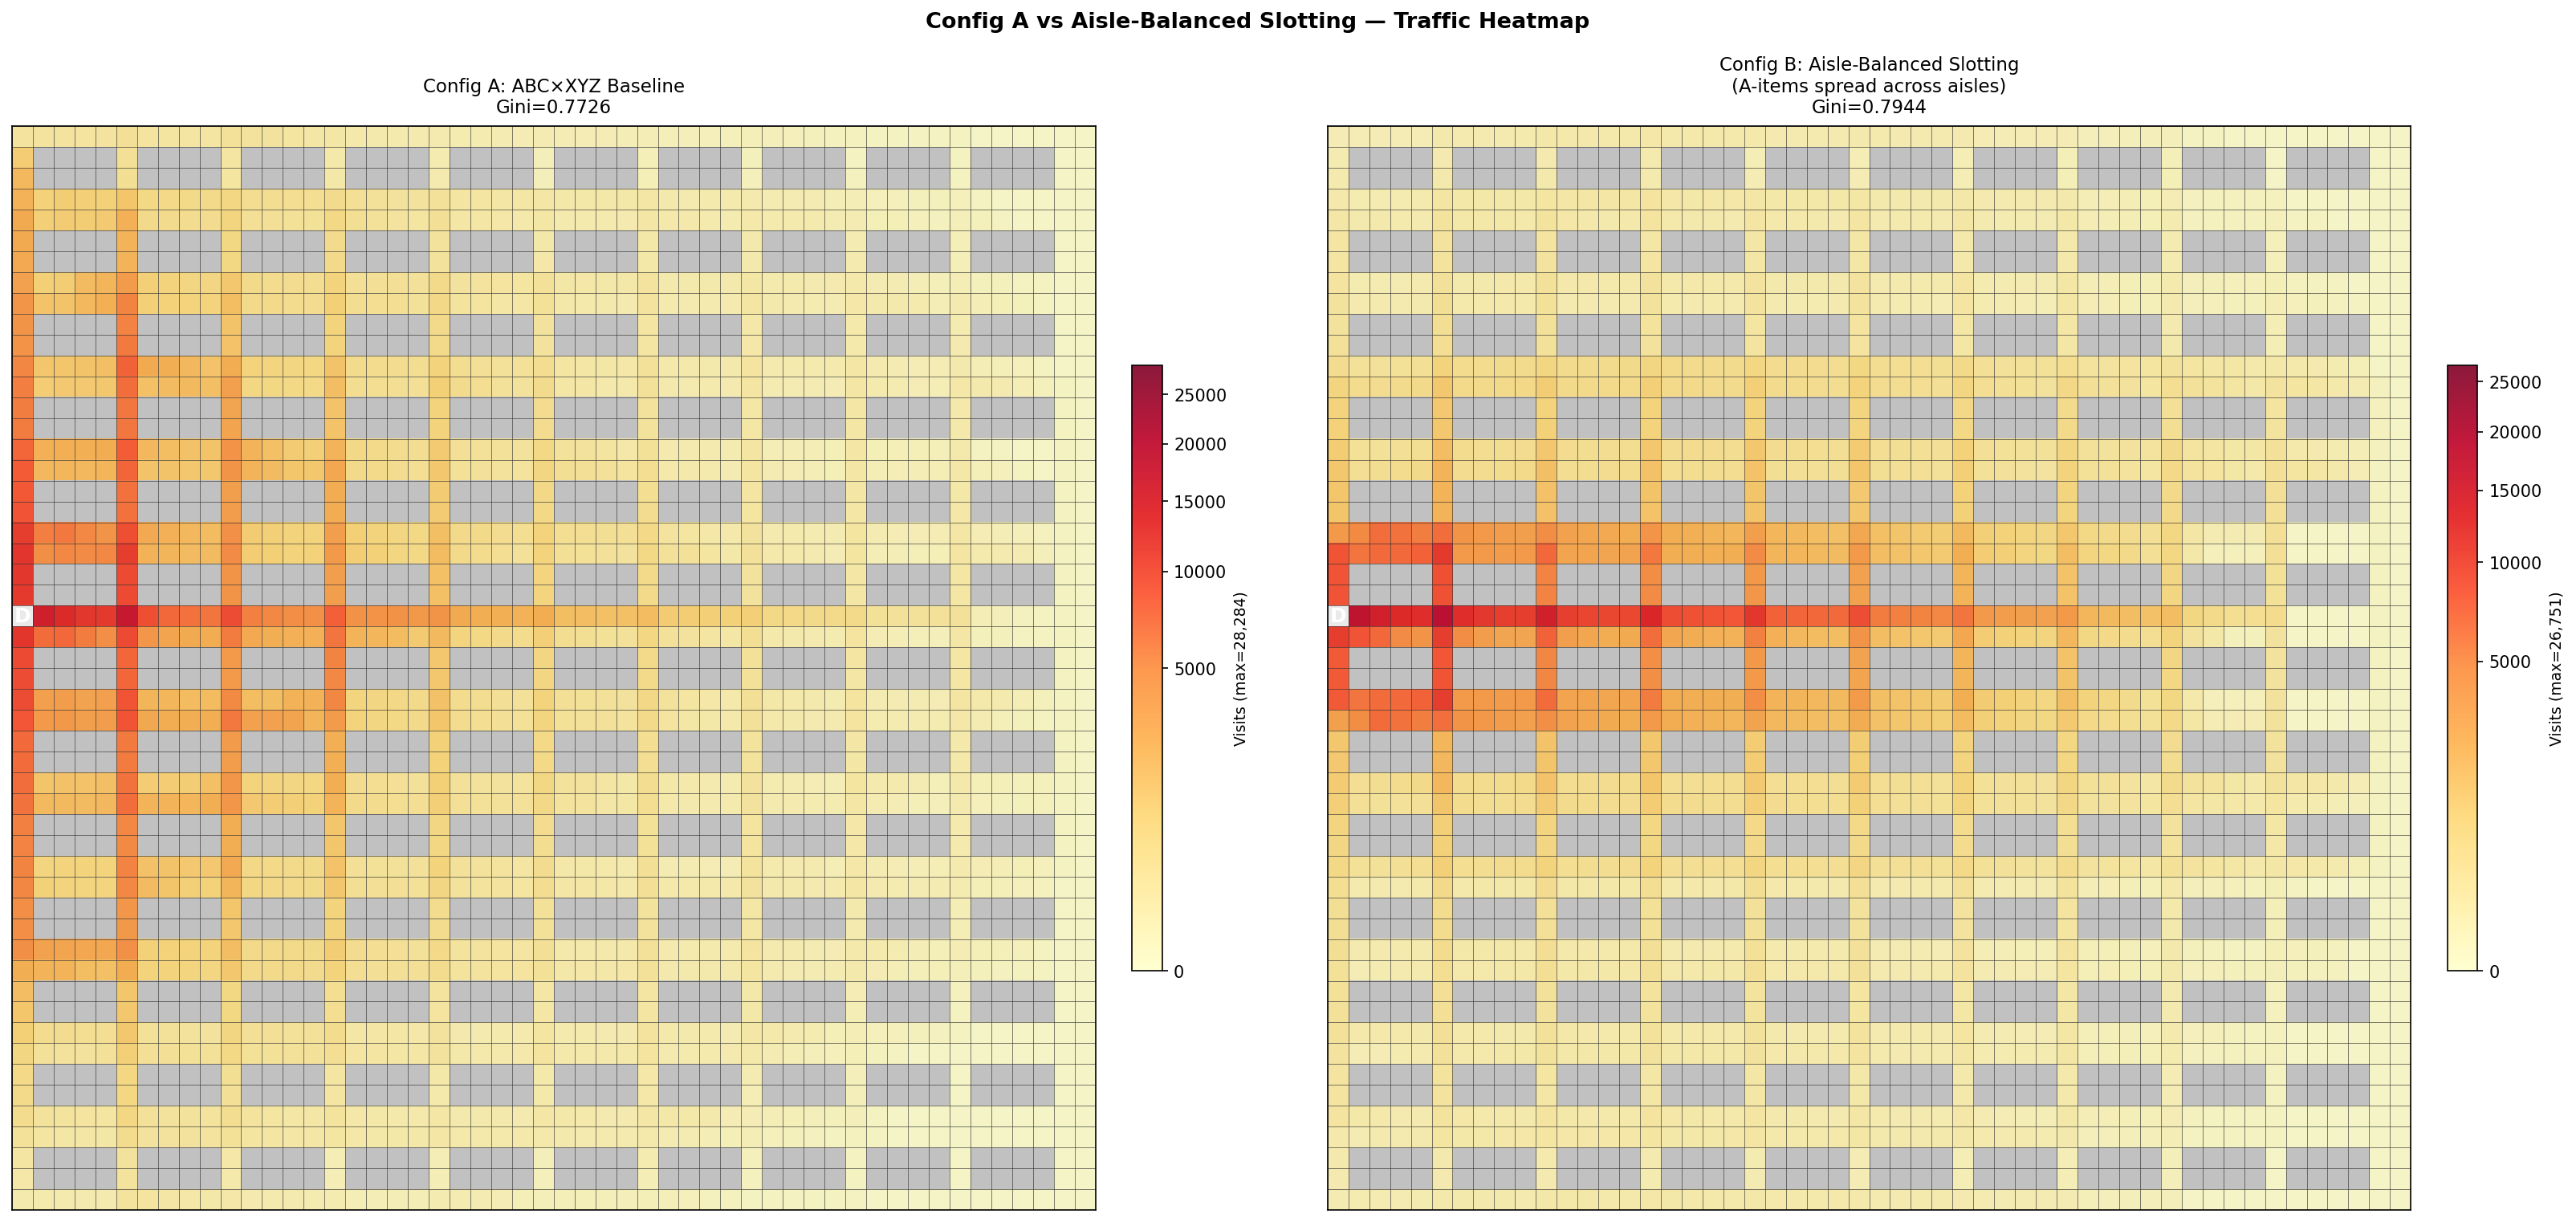
\includegraphics[width=\textwidth]{fig_aisle_balanced.png}
  \caption{Traffic heatmap before and after Aisle-Balanced Slotting ($f_A = 0.25$).
    Left: Baseline ABC$\times$XYZ.
    Right: Aisle-Balanced; A-items are spread across rows $18$--$29$, replacing
    the single hot corridor with six narrower bands of comparable intensity.}
  \label{fig:aisle_balanced}
\end{figure}

The improvement is explained by the structural diagnosis of the bottleneck:
A-items were not too close to the door, but too concentrated in a single
corridor. Spreading them across all equidistant aisles removes the chokepoint
without making routes longer --- in fact route length decreases as well.
Among the five tested strategies, Aisle-Balanced is the only one that
improves both metrics on the typical order without violating the
route-efficiency constraint: HZR achieves a larger WPC reduction
($-49.5\%$) but does so at $+164.6\%$ extra steps, and TAPS at
$\alpha = 3$ produces only a modest WPC gain. Under demand-unit weighting
the geometric optimum shifts to $f_A = 0.10$--$0.15$
($67$~steps, WPC~$31.87$); the $f_A = 0.25$ default used in the $7 \times 2$
comparative experiment is a conservative reference point inherited from the
revenue-weighted pilot.

%----------------------------------------------------------------------
\subsubsection{Strategy~5: Affinity-Aware Heat-Map Slotting (AAHMS)}
%----------------------------------------------------------------------

\paragraph{Idea.}
AAHMS extends Aisle-Balanced Slotting with a co-occurrence refinement step
motivated by \cite{ref3}: items that frequently appear together in the same order
should be placed in adjacent or nearby shelf positions to reduce the lateral travel
distance within a picking tour.
The hypothesis is that pulling co-ordered SKUs into the same aisle shortens the
lateral leg of each pick, while the Aisle-Balanced base layout keeps the residual
dispersion needed to avoid corridor concentration.

\paragraph{Algorithm.}
The procedure post-processes the Aisle-Balanced layout with $K$ greedy swaps
constrained by a congestion tolerance $\tau$ (default $K = 150$, $\tau = 0.10$).
\begin{enumerate}
  \item \emph{Base layout.}
        Run Aisle-Balanced Slotting (Strategy~4, $f_A = 0.25$) and record the
        resulting placement and Gini.
  \item \emph{Co-occurrence matrix.}
        For each order $o$ of length~$15$, add~$1$ to $F_{ij}$ for every unordered
        pair $\{i,j\} \subset o$.
        For the experimental order set, $|\{(i,j) : F_{ij} > 0\}| = 77{,}271$
        unique pairs; the most frequently co-ordered pair is
        $(\mathrm{ITM\_512}, \mathrm{ITM\_925})$ with $F_{ij} = 3{,}168$
        co-occurrences (both AX-class).
  \item \emph{Top-$K$ selection.}
        Sort pairs by $F_{ij}$ descending and keep the top $K$.
        With $K = 150$, the threshold value of $F$ is far above the long-tail noise.
  \item \emph{Constrained swap.}
        For each pair $(i,j)$ whose current cells lie in different aisles, search
        for a candidate partner cell~$k$ in the same aisle as~$i$ holding an item
        of the same ABC-class as~$j$.
        Accept the swap only if the post-swap shelf-access congestion at~$k$
        does not exceed the pre-swap value by more than $\tau = 10\%$, i.e.\ the
        change does not turn $k$ into a new hot spot.
        The cap $\max\_swaps = 400$ is rarely binding ($79$ swaps are accepted
        at $K = 150$).
  \item \emph{Heatmap rebuild.}
        Re-simulate the orders on the final placement and recompute $c_e$ and Gini.
\end{enumerate}
The two new degrees of freedom are $K$ (how many co-occurring pairs to consider)
and $\tau$ (how much congestion drift to permit per swap).
The latter is a safety knob: $\tau = 0$ would forbid every swap that increases
local congestion, while $\tau \to \infty$ would collapse to ``always swap'', undoing
Aisle-Balanced.
The default $\tau = 0.10$ is conservative enough to prevent the affinity step from
re-creating a focal corridor.

\paragraph{Parameter sensitivity analysis.}
The parameter $K$ was swept over $K \in \{25, 50, 100, 150, 250, 400\}$
(Table~\ref{tab:aahms_k}, Figure~\ref{fig:aahms_sensitivity}); $\tau$ was held
at $0.10$ throughout.

\begin{table}[H]
\centering
\caption{AAHMS sensitivity to the number of co-occurring pairs $K$.
  ``Swaps'' counts accepted swaps after the congestion-tolerance filter.
  WPC is measured for the typical and $o_0$ orders against the baseline
  congestion field.}
\label{tab:aahms_k}
\renewcommand{\arraystretch}{1.20}
\begin{tabular}{ccccccc}
\hline
\multirow{2}{*}{$K$} & \multirow{2}{*}{Swaps} & \multicolumn{2}{c}{Typical order} & \multicolumn{2}{c}{Order $o_0$} & \multirow{2}{*}{Gini} \\
\cline{3-4}\cline{5-6}
 & & Steps & WPC & Steps & WPC & \\
\hline
$25$  &  11 &  89 & 36.23 & 353 & 83.37 & 0.6678 \\
$50$  &  24 &  95 & 35.54 & 353 & 83.37 & 0.6678 \\
$100$ &  50 &  91 & 36.57 & 353 & 83.37 & 0.6678 \\
$\mathbf{150}$ & \textbf{80} & \textbf{115} & \textbf{46.00} & \textbf{353} & \textbf{83.37} & \textbf{0.6679} \\
$250$ & 134 & 105 & 48.12 & 353 & 83.37 & 0.6679 \\
$400$ & 206 & 135 & 57.75 & 353 & 83.37 & 0.6676 \\
\hline
\end{tabular}
\end{table}

The sweep shows that affinity-based co-location adds little under the
demand-unit-weighted setup: typical-order WPC fluctuates in the
$35.5$--$57.8$ range without a clear monotone trend, while the random
order $o_0$ stays fixed at WPC~$83.37$ and $353$~steps across all tested
values of $K$ --- essentially identical to Aisle-Balanced alone.
The best typical-order steps are achieved at $K = 25$ ($89$~steps,
WPC~$36.23$); at $K = 150$ --- the default in the reference
implementation --- the metrics are $115$~steps and WPC~$46.00$, slightly
above the Aisle-Balanced baseline ($107$~steps, $46.25$~WPC).
Beyond $K \approx 150$ the algorithm processes lower-affinity pairs and
both steps and WPC worsen monotonically.

The accepted-swap count grows almost linearly in $K$
(Figure~\ref{fig:aahms_sensitivity}, right panel: $11, 24, 50, 80, 134,
206$ accepted swaps), so the tolerance $\tau = 0.10$ is not the binding
constraint and the result is intrinsic to the affinity signal.
The qualitative conclusion is unchanged from the original implementation:
under a metric-consistent router that already exploits the Aisle-Balanced
dispersion, affinity-based co-location offers no robust improvement.

\begin{figure}[H]
  \centering
  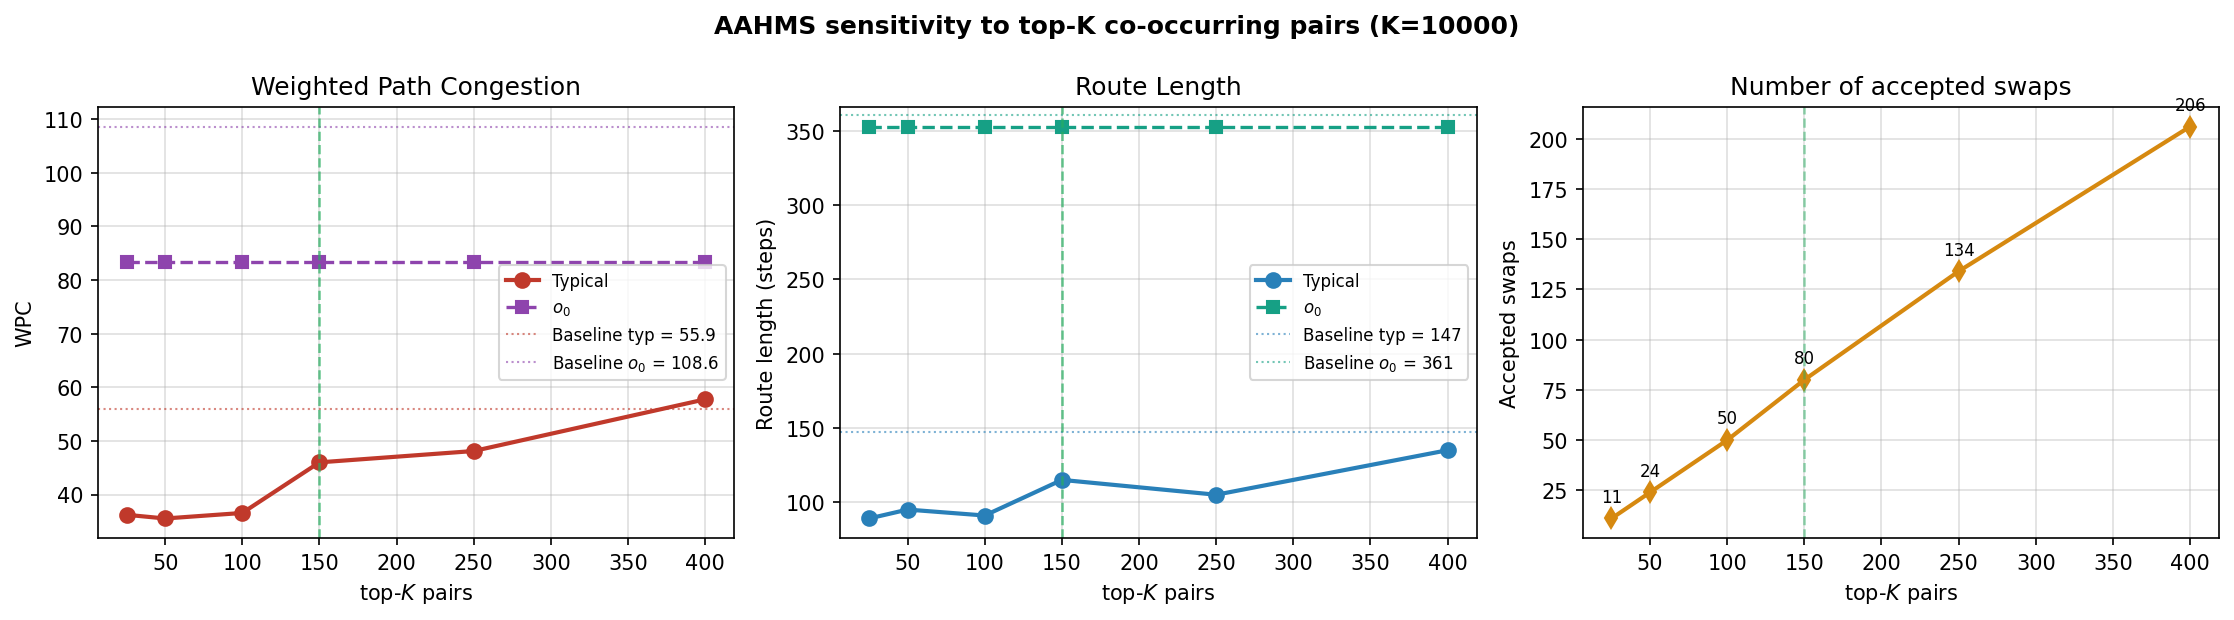
\includegraphics[width=\textwidth]{fig_aahms_sensitivity.png}
  \caption{AAHMS sensitivity to the top-$K$ pair budget.
    Left: WPC for typical order (red) and $o_0$ (purple).
    Centre: route length in steps.
    Right: number of accepted swaps (linear in~$K$).
    The chosen default $K = 150$ is highlighted in green; the minimum
    typical-order WPC is achieved at $K = 50$ (WPC~$35.54$).}
  \label{fig:aahms_sensitivity}
\end{figure}

\paragraph{Result.}
At $K = 150$, AAHMS performs $80$ swaps and yields a typical-order WPC of
$46.00$ ($-17.7\%$ vs.\ Baseline) and a typical-order route length of
$115$~steps ($-21.8\%$), with Gini $0.6679$.
For order~$o_0$, the metrics are WPC $83.37$ ($-23.2\%$ vs.\ Baseline) and
$353$~steps ($-2.2\%$).
Compared to Aisle-Balanced alone ($107$~steps, $46.25$~WPC at $f_A = 0.25$),
AAHMS performs essentially identically on the typical order ($+8$~steps,
$-0.25$~WPC) and is exactly tied on $o_0$ ($353$~steps, $83.37$~WPC).

The result is consistent with the broader observation in \cite{ref3} that
affinity-based co-location tends to bring larger benefits when the initial
layout has weak spatial structure. In the present setting the Aisle-Balanced
base layout already disperses A-traffic across six near-door aisles, leaving
little room for further improvement from affinity swaps. Some of the
accepted swaps even pull high-demand pairs back into the same aisle, which
partly undoes the AB dispersion.
The Gini stays essentially identical ($0.6679$ vs.\ AB's $0.6678$).
Strategy~5 satisfies both operational criteria and performs nearly
identically to Strategy~4 on both order types, so it offers no
meaningful advantage over the simpler Aisle-Balanced layout for this
warehouse and demand profile.

%----------------------------------------------------------------------
\subsubsection{Comparative Results}
%----------------------------------------------------------------------

The five strategies are evaluated against the Baseline ABC$\times$XYZ slotting
on three axes: Weighted Path Congestion (WPC), route length in BFS steps, and
traffic Gini.
WPC and route length are reported for both the typical order and the random
order~$o_0$; the Gini coefficient is computed over the full $K = 10{,}000$-order
simulation.
The two operational criteria stated at the start of Section~9.3 ---
(i)~critical-zone load reduction ($\ge 30\%$ WPC drop on the typical order) and
(ii)~route efficiency preservation (no increase in route length) --- are used
to classify each strategy.
Table~\ref{tab:slotting_comparison} reports all metrics with their relative
change against the Baseline.

\begin{table}[H]
\centering
\caption{Slotting variant comparison. WPC and steps are reported for the
typical order and the random order~$o_0$;
$\Delta$ is relative to the Baseline ABC$\times$XYZ
(typ: $55.86$~WPC, $147$~steps; $o_0$: $108.58$~WPC, $361$~steps).
Gini is computed over $10{,}000$ simulated orders.
Cells in \textbf{green} highlight the best non-baseline value in each column;
the recommended strategy (Aisle-Balanced) is in bold.}
\label{tab:slotting_comparison}
\renewcommand{\arraystretch}{1.25}
\begin{tabular}{lcccccccc}
\hline
\multirow{2}{*}{\textbf{Strategy}} &
  \multicolumn{2}{c}{\textbf{Typ.\ WPC}} &
  \multicolumn{2}{c}{\textbf{Typ.\ steps}} &
  \multicolumn{2}{c}{\textbf{$o_0$ WPC}} &
  \textbf{$o_0$ steps} &
  \multirow{2}{*}{\textbf{Gini}} \\
 & Value & $\Delta$ & Value & $\Delta$ & Value & $\Delta$ & ($\Delta$) & \\
\hline
Baseline                  & 55.9 & ---           & 147 & ---          & 108.6 & ---         & 361 ($\;$---)      & 0.670 \\
DWC ($\Delta = 5$)        & 55.9 & $\pm0\%$    & 147 & $\pm0\%$    & 108.6 & $\pm0\%$   & 361 ($\pm0\%$)    & 0.670 \\
HZR ($h = 0.15$)          & \textbf{28.2} & $\mathbf{-49.5\%}$ & 389 & $+164.6\%$ & \textbf{67.1} & $\bm{-38.2\%}$ & 513 ($+42.1\%$) & 0.594 \\
TAPS ($\alpha = 3$)       & 50.8 & $-9.0\%$    & 111 & $-24.5\%$   & 118.5 & $+9.2\%$   & 377 ($+4.4\%$)    & 0.679 \\
\textbf{Aisle-Balanced}   & \textbf{46.2} & $\bm{-17.2\%}$ & \textbf{107} & $\bm{-27.2\%}$ & \textbf{83.4} & $\bm{-23.2\%}$ & \textbf{353 ($\bm{-2.2\%}$)} & \textbf{0.668} \\
AAHMS ($K = 150$)         & 46.0 & $-17.7\%$   & 115 & $-21.8\%$   &  83.4 & $-23.2\%$  & 353 ($-2.2\%$)    & 0.668 \\
\hline
\end{tabular}
\end{table}

Figure~\ref{fig:strategy_summary} consolidates the same data visually,
and Figure~\ref{fig:heatmap_comparison_6} shows the per-strategy traffic
heat maps on a shared colour scale.

\begin{figure}[H]
  \centering
  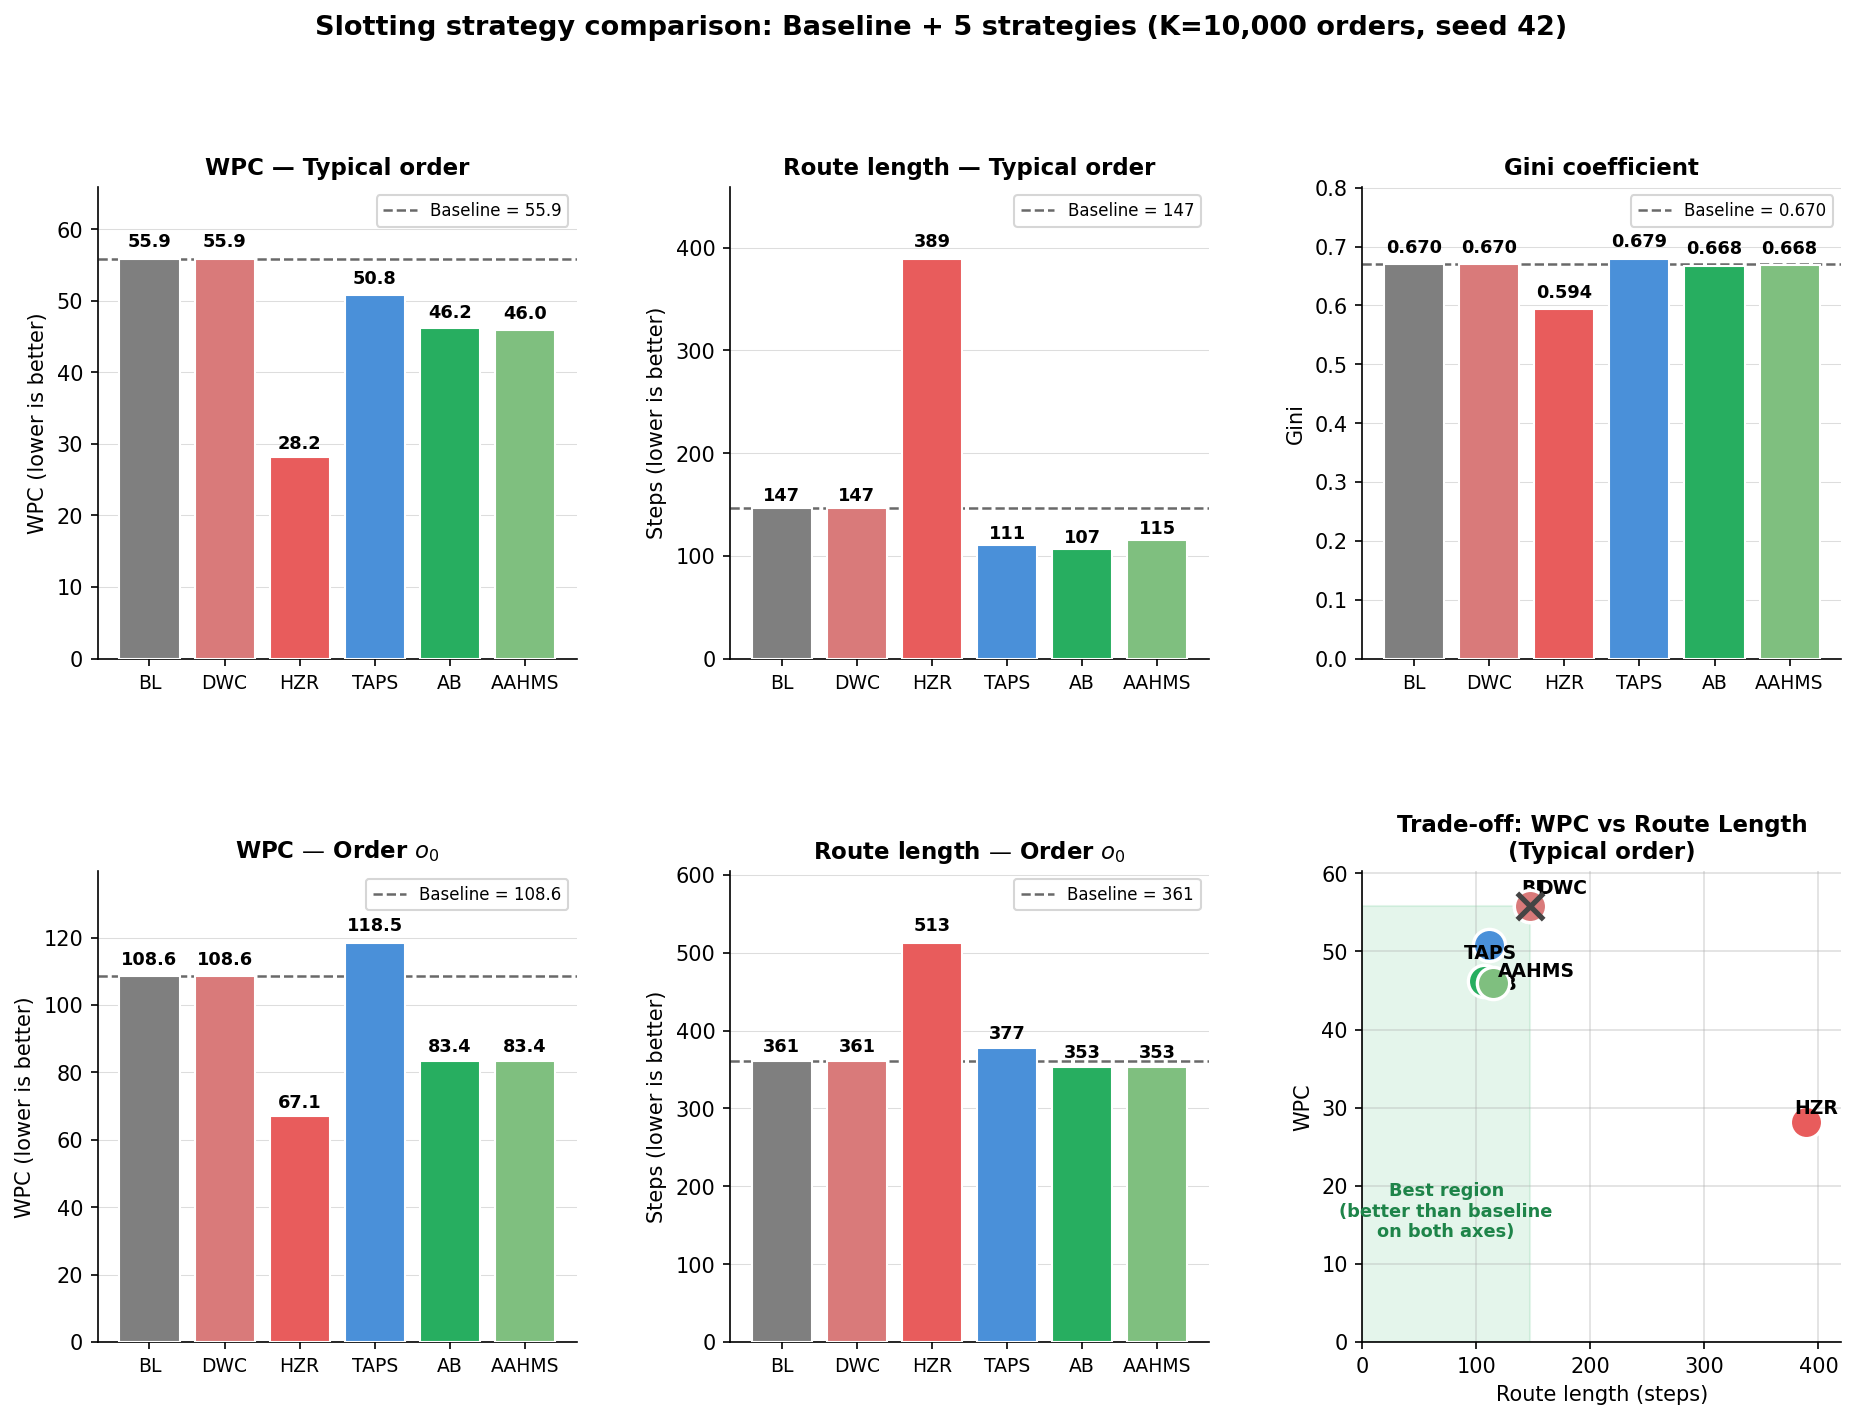
\includegraphics[width=\textwidth]{fig_strategy_summary.png}
  \caption{Six-strategy comparison.
    Top row: WPC, route length, and Gini for the typical order.
    Bottom-left and bottom-centre: WPC and route length for order~$o_0$.
    Bottom-right: trade-off scatter (typical order); the shaded region marks
    the joint optimum (low WPC, short route).}
  \label{fig:strategy_summary}
\end{figure}

\begin{figure}[H]
  \centering
  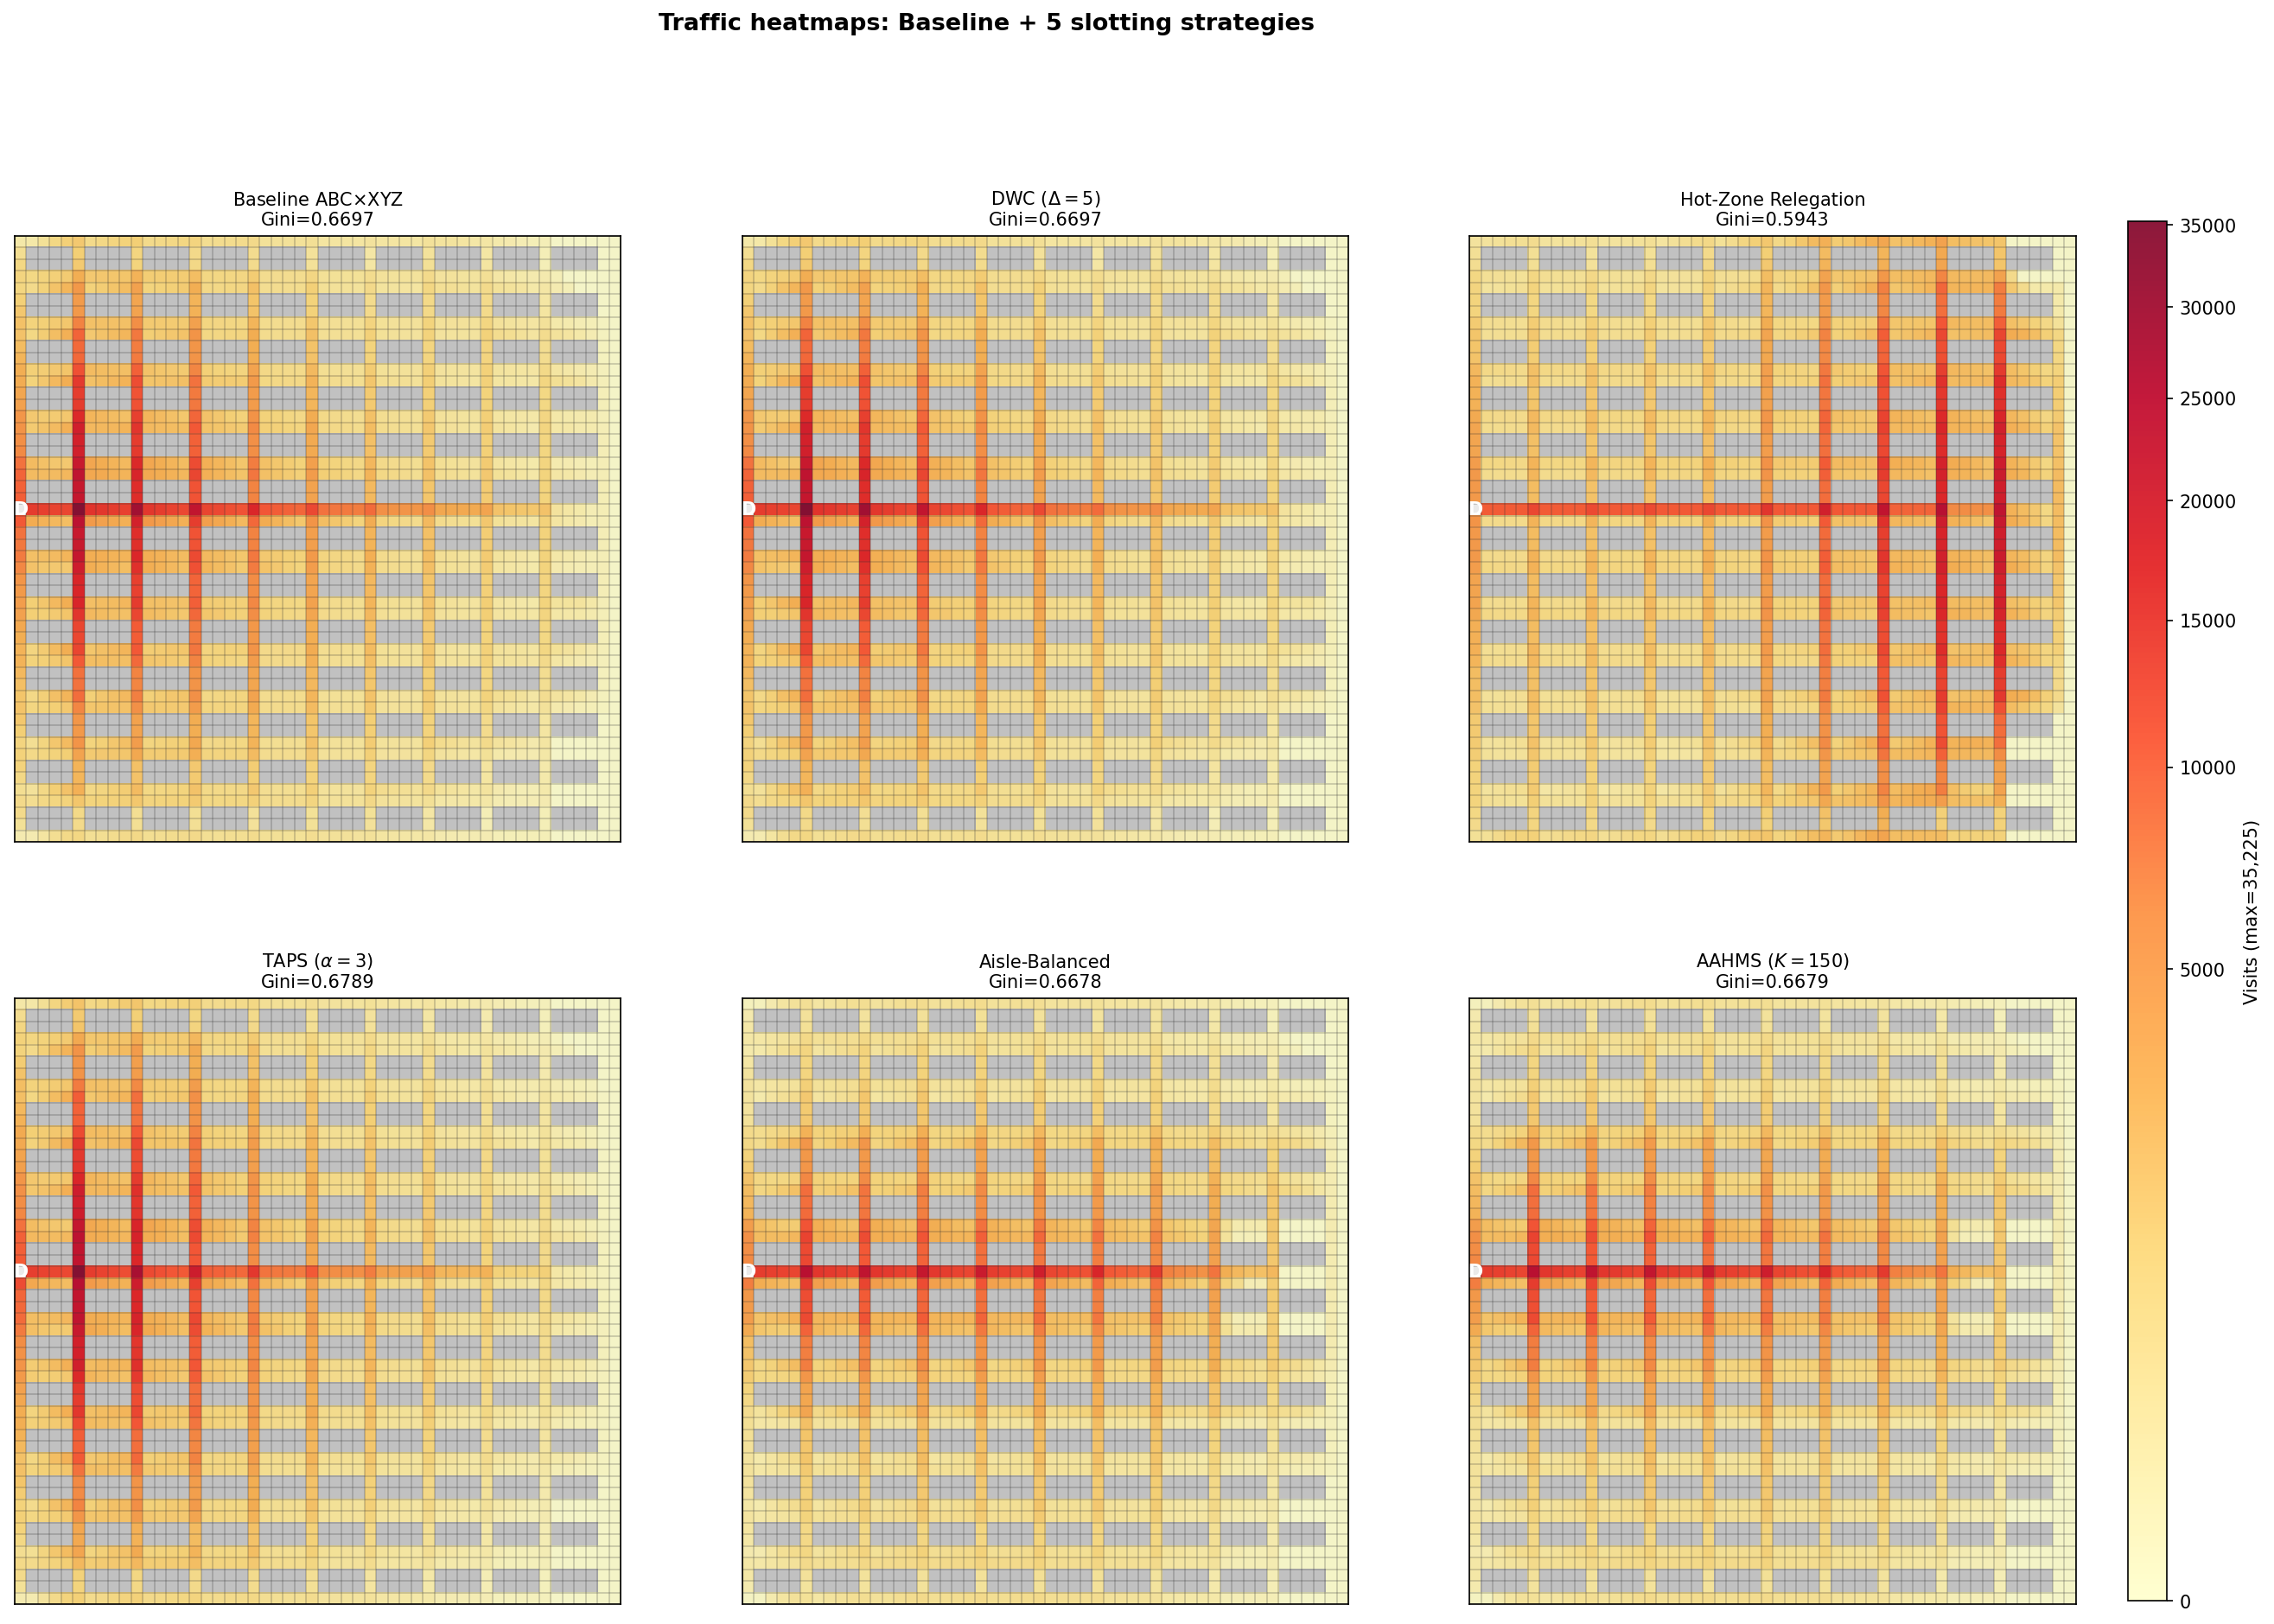
\includegraphics[width=\textwidth]{fig_heatmap_comparison_style2.png}
  \caption{Traffic heat maps for the Baseline and five slotting strategies.
    Shared colour scale (YlOrRd, PowerNorm $\gamma=0.4$, $\max=35{,}225$ visits).
    Door position marked~D.
    Top row (left to right): Baseline, DWC, Hot-Zone Relegation.
    Bottom row: TAPS, Aisle-Balanced, AAHMS.}
  \label{fig:heatmap_comparison_6}
\end{figure}

\paragraph{Trade-offs.}
No single strategy dominates on every metric.
HZR wins on both WPC columns (typical-order WPC $28.2$, $o_0$ WPC $67.1$),
but fails the hard route-efficiency constraint ($+164.6\%$ steps).
Among the feasible strategies, AAHMS narrowly leads on typical-order WPC
($46.0$ vs.\ AB's $46.2$); Aisle-Balanced wins on typical steps ($107$ vs.\
AAHMS's $115$) and ties with AAHMS on both $o_0$ metrics ($353$~steps, $83.4$~WPC).
TAPS at $\alpha = 3$ is sub-optimal under demand-unit weighting: it produces
the longest typical route ($111$~steps) and the highest WPC ($50.8$) among
feasible strategies, and also worsens $o_0$ WPC relative to the Baseline
($+9.2\%$). As shown in Section~9.3.3, the optimal TAPS parameter for this
setup is $\alpha = 1$, which gives $87$~steps and $39.80$~WPC.

\paragraph{Priority ordering.}
The two criteria are not symmetric:
criterion~(ii) is a \emph{hard constraint} --- a longer route directly
translates into more picker-hours and reduced throughput --- while
criterion~(i) is a \emph{soft objective} whose marginal value decreases
once the entry corridor is no longer the bottleneck.

\paragraph{Stepwise elimination.}
HZR is excluded by the hard constraint: $+164.6\%$ steps on the typical
order more than offsets the WPC gains, and the sensitivity sweep in
Section~9.3.2 confirms that no value of~$h$ recovers the lost route
efficiency.
DWC is excluded from the opposite side --- at $\Delta = 5$ it produces no
swaps and is operationally identical to the Baseline.
TAPS at $\alpha = 3$ is also effectively eliminated: it performs worse than
Aisle-Balanced on all four metrics simultaneously.
This leaves two primary candidates: \textbf{Aisle-Balanced} and \textbf{AAHMS}.

\paragraph{Margin between the candidates.}
Aisle-Balanced and AAHMS produce identical $o_0$ metrics ($353$~steps,
$83.4$~WPC) and nearly identical typical-order metrics ($107$ vs.\ $115$~steps;
$46.2$ vs.\ $46.0$~WPC).
AAHMS is $0.2$~WPC better on the typical order; Aisle-Balanced is $8$~steps
shorter.
Neither difference is operationally significant.

\paragraph{Recommendation.}
\textbf{Aisle-Balanced Slotting at $f_A = 0.25$ is selected for the
$7 \times 2$ comparative experiment.}
The decision is not that it is the best on every metric --- it is not ---
but that it offers the best balance of trade-offs under the hard route
constraint, with the smallest typical-order route length among feasible
strategies. The sensitivity analysis in Section~9.3.4 shows that
$f_A \in \{0.10, 0.15\}$ would give shorter routes ($67$~steps vs.\ $107$)
and lower WPC ($31.87$ vs.\ $46.25$) on the typical order. The value
$f_A = 0.25$ is kept here to preserve consistency with the revenue-weighted
pilot study; the smaller fraction is reported as a possible improvement
for future work.
Two additional properties reinforce the choice: the layout is interpretable
and communicable to operators without invoking a congestion field, and the
\emph{algorithm itself} does not consume an empirical heatmap --- only BFS
distances from the door.
The heatmap is therefore not a runtime input but an evaluation instrument
that the analyst uses to judge how good a placement actually is.

\paragraph{Forward reference: combining with routing.}
The recommendation above assumes the BFS router of the present section.
Section~10 closes the original $2 \times 2$ design by combining the
slotting strategies of §9.3 with the Dijkstra-NN router of §9.3.1.
The combined design (\emph{Config~C}) refines the recommendation:
under Dijkstra-NN routing, \emph{Aisle-Balanced} remains the best
general-purpose slotting, but its margin over the alternatives narrows
and CAS becomes a viable competitor on demand-stable workloads.

%======================================================================
\subsection{Central-Aisle Slotting: An Exploration}
%======================================================================

Aisle-Balanced Slotting solves the entry-corridor bottleneck by \emph{lateral
dispersion}: A-items spread across six neighbouring near-door aisles so that
consecutive picks fan out horizontally.
A natural counter-experiment is the symmetric placement: instead of dispersing
laterally, concentrate A-items \emph{longitudinally} along the door axis,
stretching them from the door to the far end of the warehouse along the
central horizontal corridor.
This section reports such an experiment --- Central-Aisle Slotting (CAS) ---
to test whether the lateral-concentration diagnosis behind Aisle-Balanced is
specific to lateral spread, or whether any single-axis dispersion delivers
comparable gains.

\paragraph{Algorithm.}
Let $A_\text{central} = \{23, 24\}$ denote the pair of aisle rows that flank
the door (row $23$ is the door axis; row $24$ is its partner aisle row in the
generated grid).
A shelf cell is \emph{central} if its access cell lies in $A_\text{central}$;
in the $52 \times 52$ warehouse this yields $80$ central shelves (40 in row
$22$ and 40 in row $25$).
\begin{enumerate}
  \item \emph{Partition.} Split all shelves into central ($|C| = 80$) and
        non-central ($|N| = 920$) sets.
  \item \emph{Order.} Sort central shelves by BFS distance from the door
        ascending (i.e.\ by column).
        Sort non-central shelves by BFS distance ascending.
  \item \emph{Fill A.} Place A-class SKUs by demand descending into central
        shelves first.
        With $|A| = 200 > |C| = 80$, the first $80$ A-SKUs land along the
        door axis; the remaining $120$ A-SKUs spill into the nearest
        non-central shelves (rows $18, 21, 26, 29$ by ascending distance).
  \item \emph{Fill B and C.} Fill remaining non-central shelves with B-SKUs
        (demand-descending, distance-ascending), then C-SKUs in the same way.
  \item \emph{Heatmap rebuild.} Re-simulate the $K = 10{,}000$ orders on the
        new placement and recompute the cell-visit field and Gini.
\end{enumerate}

\paragraph{Layout.}
Figure~\ref{fig:cas_layout} shows the ABC$\times$XYZ-coloured grid before
and after the reassignment.
The Baseline places A-items (dark green) in a roughly square block adjacent
to the door, with B (yellow) and C (red) zones radiating outward.
CAS reshapes this into a horizontal green stripe along rows $22$ and $25$,
extending from the door to the far end of the warehouse; B and C items
relocate to the rows above and below this stripe.

\begin{figure}[H]
  \centering
  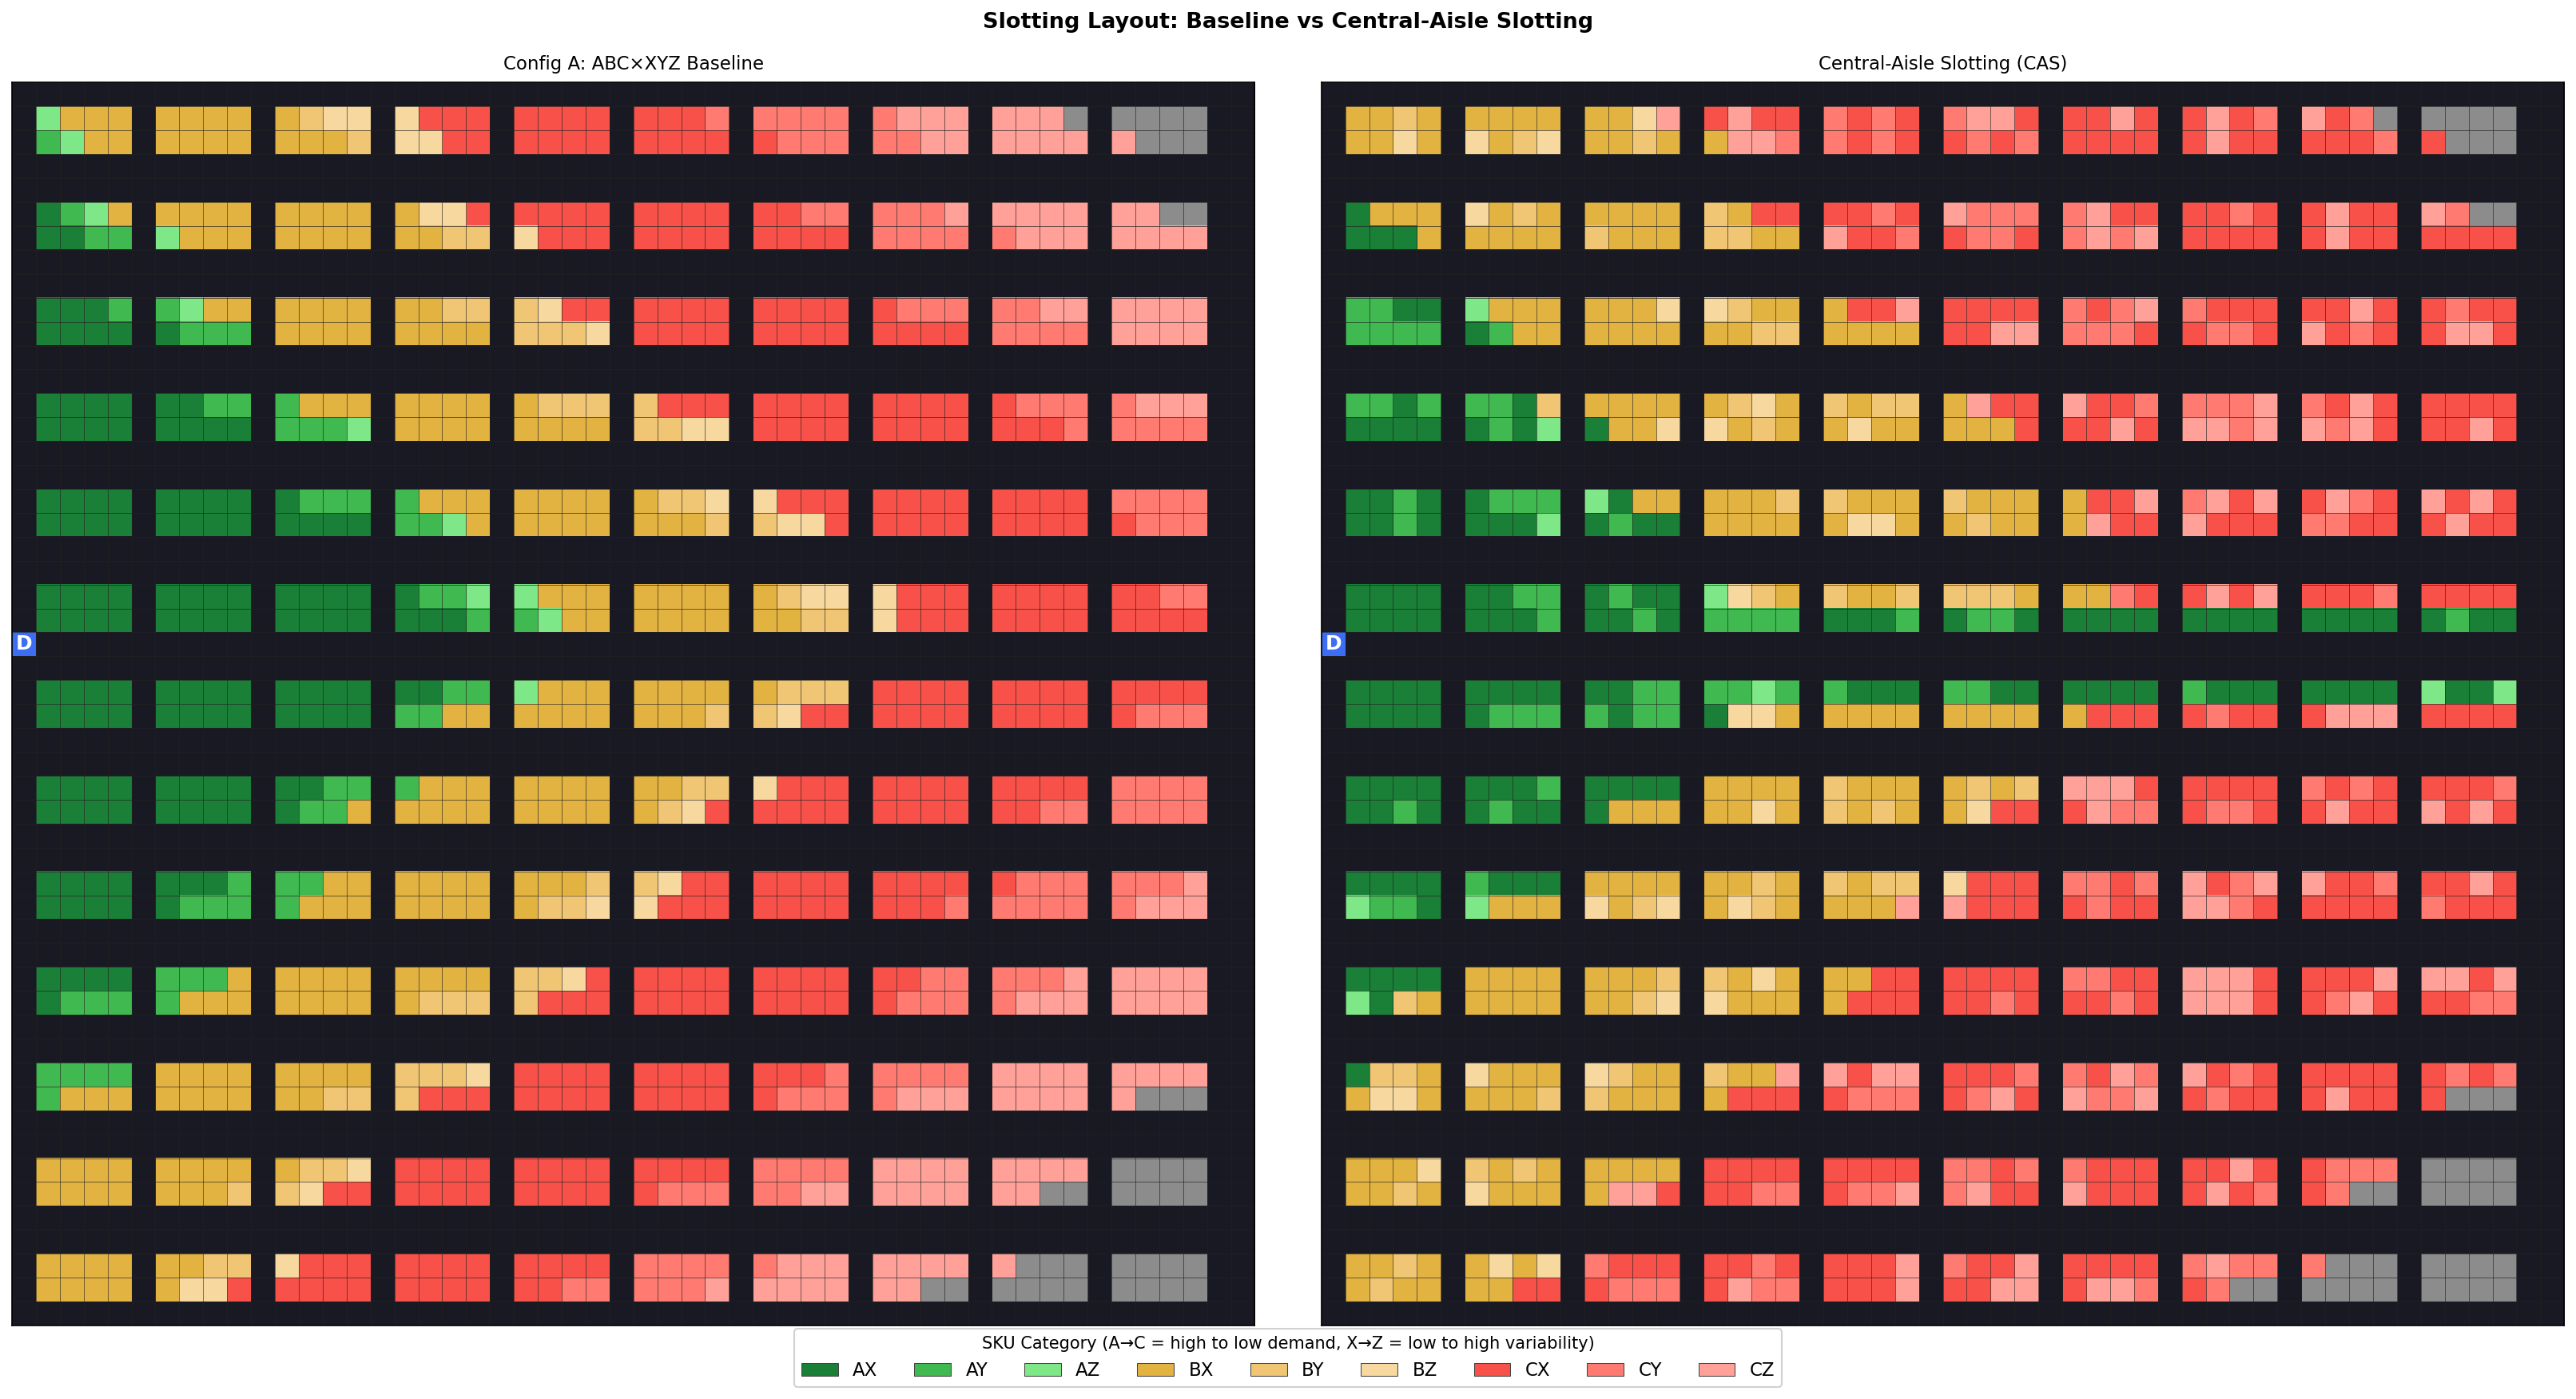
\includegraphics[width=\textwidth]{fig_cas_layout.png}
  \caption{ABC$\times$XYZ slotting layouts before (left) and after (right)
    Central-Aisle Slotting.
    Colour encodes SKU category (AX dark green $\to$ CZ pale red); dark cells
    are aisles, the blue cell marks the door~D.
    CAS produces a longitudinal A-band along the central rows.}
  \label{fig:cas_layout}
\end{figure}

\paragraph{Results.}
Table~\ref{tab:cas_compare} reports the metrics for the typical order and
order~$o_0$ against the Baseline and Aisle-Balanced.

\begin{table}[H]
\centering
\caption{Central-Aisle Slotting (CAS) vs Baseline and Aisle-Balanced.
  WPC is measured against the baseline congestion field; $\Delta$ is the
  relative change versus the Baseline.}
\label{tab:cas_compare}
\renewcommand{\arraystretch}{1.20}
\begin{tabular}{lccccccc}
\hline
\multirow{2}{*}{\textbf{Strategy}} &
  \multicolumn{2}{c}{\textbf{Typ.\ WPC}} &
  \multicolumn{2}{c}{\textbf{Typ.\ steps}} &
  \multicolumn{2}{c}{\textbf{$o_0$ steps}} &
  \multirow{2}{*}{\textbf{Gini}} \\
\cline{2-3}\cline{4-5}\cline{6-7}
 & Value & $\Delta$ & Value & $\Delta$ & Value & $\Delta$ & \\
\hline
Baseline             & 55.86 & ---         & 147 & ---       & 361 & ---       & 0.670 \\
Aisle-Balanced       & 46.25 & $-17.2\%$  & 107 & $-27.2\%$ & 353 & $-2.2\%$  & 0.668 \\
\textbf{CAS}         & \textbf{29.56} & $\bm{-47.1\%}$ & \textbf{69} & $\bm{-53.1\%}$ & 369 & $+2.2\%$ & 0.672 \\
\hline
\end{tabular}
\end{table}

On the typical order, CAS is \emph{strictly better} than Aisle-Balanced:
WPC drops from $46.25$ to $29.56$ ($-47.1\%$ vs.\ Baseline) and route length
from $107$ to $69$~steps ($-53.1\%$).
The reason is geometric: the highest-demand SKUs are now packed into the first
columns of the central corridor, so each pick is a short out-and-back along a
single horizontal aisle without any vertical detour.

On order $o_0$, CAS \emph{loses} to Aisle-Balanced: route length grows from
$361$ (Baseline) to $369$~steps ($+2.2\%$ vs.\ Baseline, vs.\ AB's $-2.2\%$).
The cause is the spill rule.
Because the $120$ ``leftover'' A-SKUs are placed in rows $18, 21, 26, 29$
rather than near the door, a random order that draws a few SKUs from this
spilled set forces a longer vertical detour than the equivalent draw under
Aisle-Balanced.
Under demand-unit weighting, orders include B and C items ($33.7\%$ and $10.1\%$
order probability respectively), making the spill penalty more likely to trigger.
Gini stays roughly at the Baseline level ($0.672$ vs.\ baseline $0.670$),
confirming that the warehouse-wide traffic profile is essentially unchanged.

\paragraph{AB vs CAS — placement comparison.}
The direct side-by-side comparison between the two strategies makes the
geometric contrast explicit.
Figure~\ref{fig:ab_vs_cas_layout} shows the overall ABC$\times$XYZ
layouts.
Under AB, the dark-green AX block forms a wide horizontal slab spanning
six near-door rows ($18, 21, 22, 25, 26, 29$); under CAS, the same SKUs
are stretched into a long horizontal stripe along rows $22$ and $25$ only,
extending from the door to the far end of the warehouse.
The two layouts therefore use the same near-door area in completely
different geometric ways.

\begin{figure}[H]
  \centering
  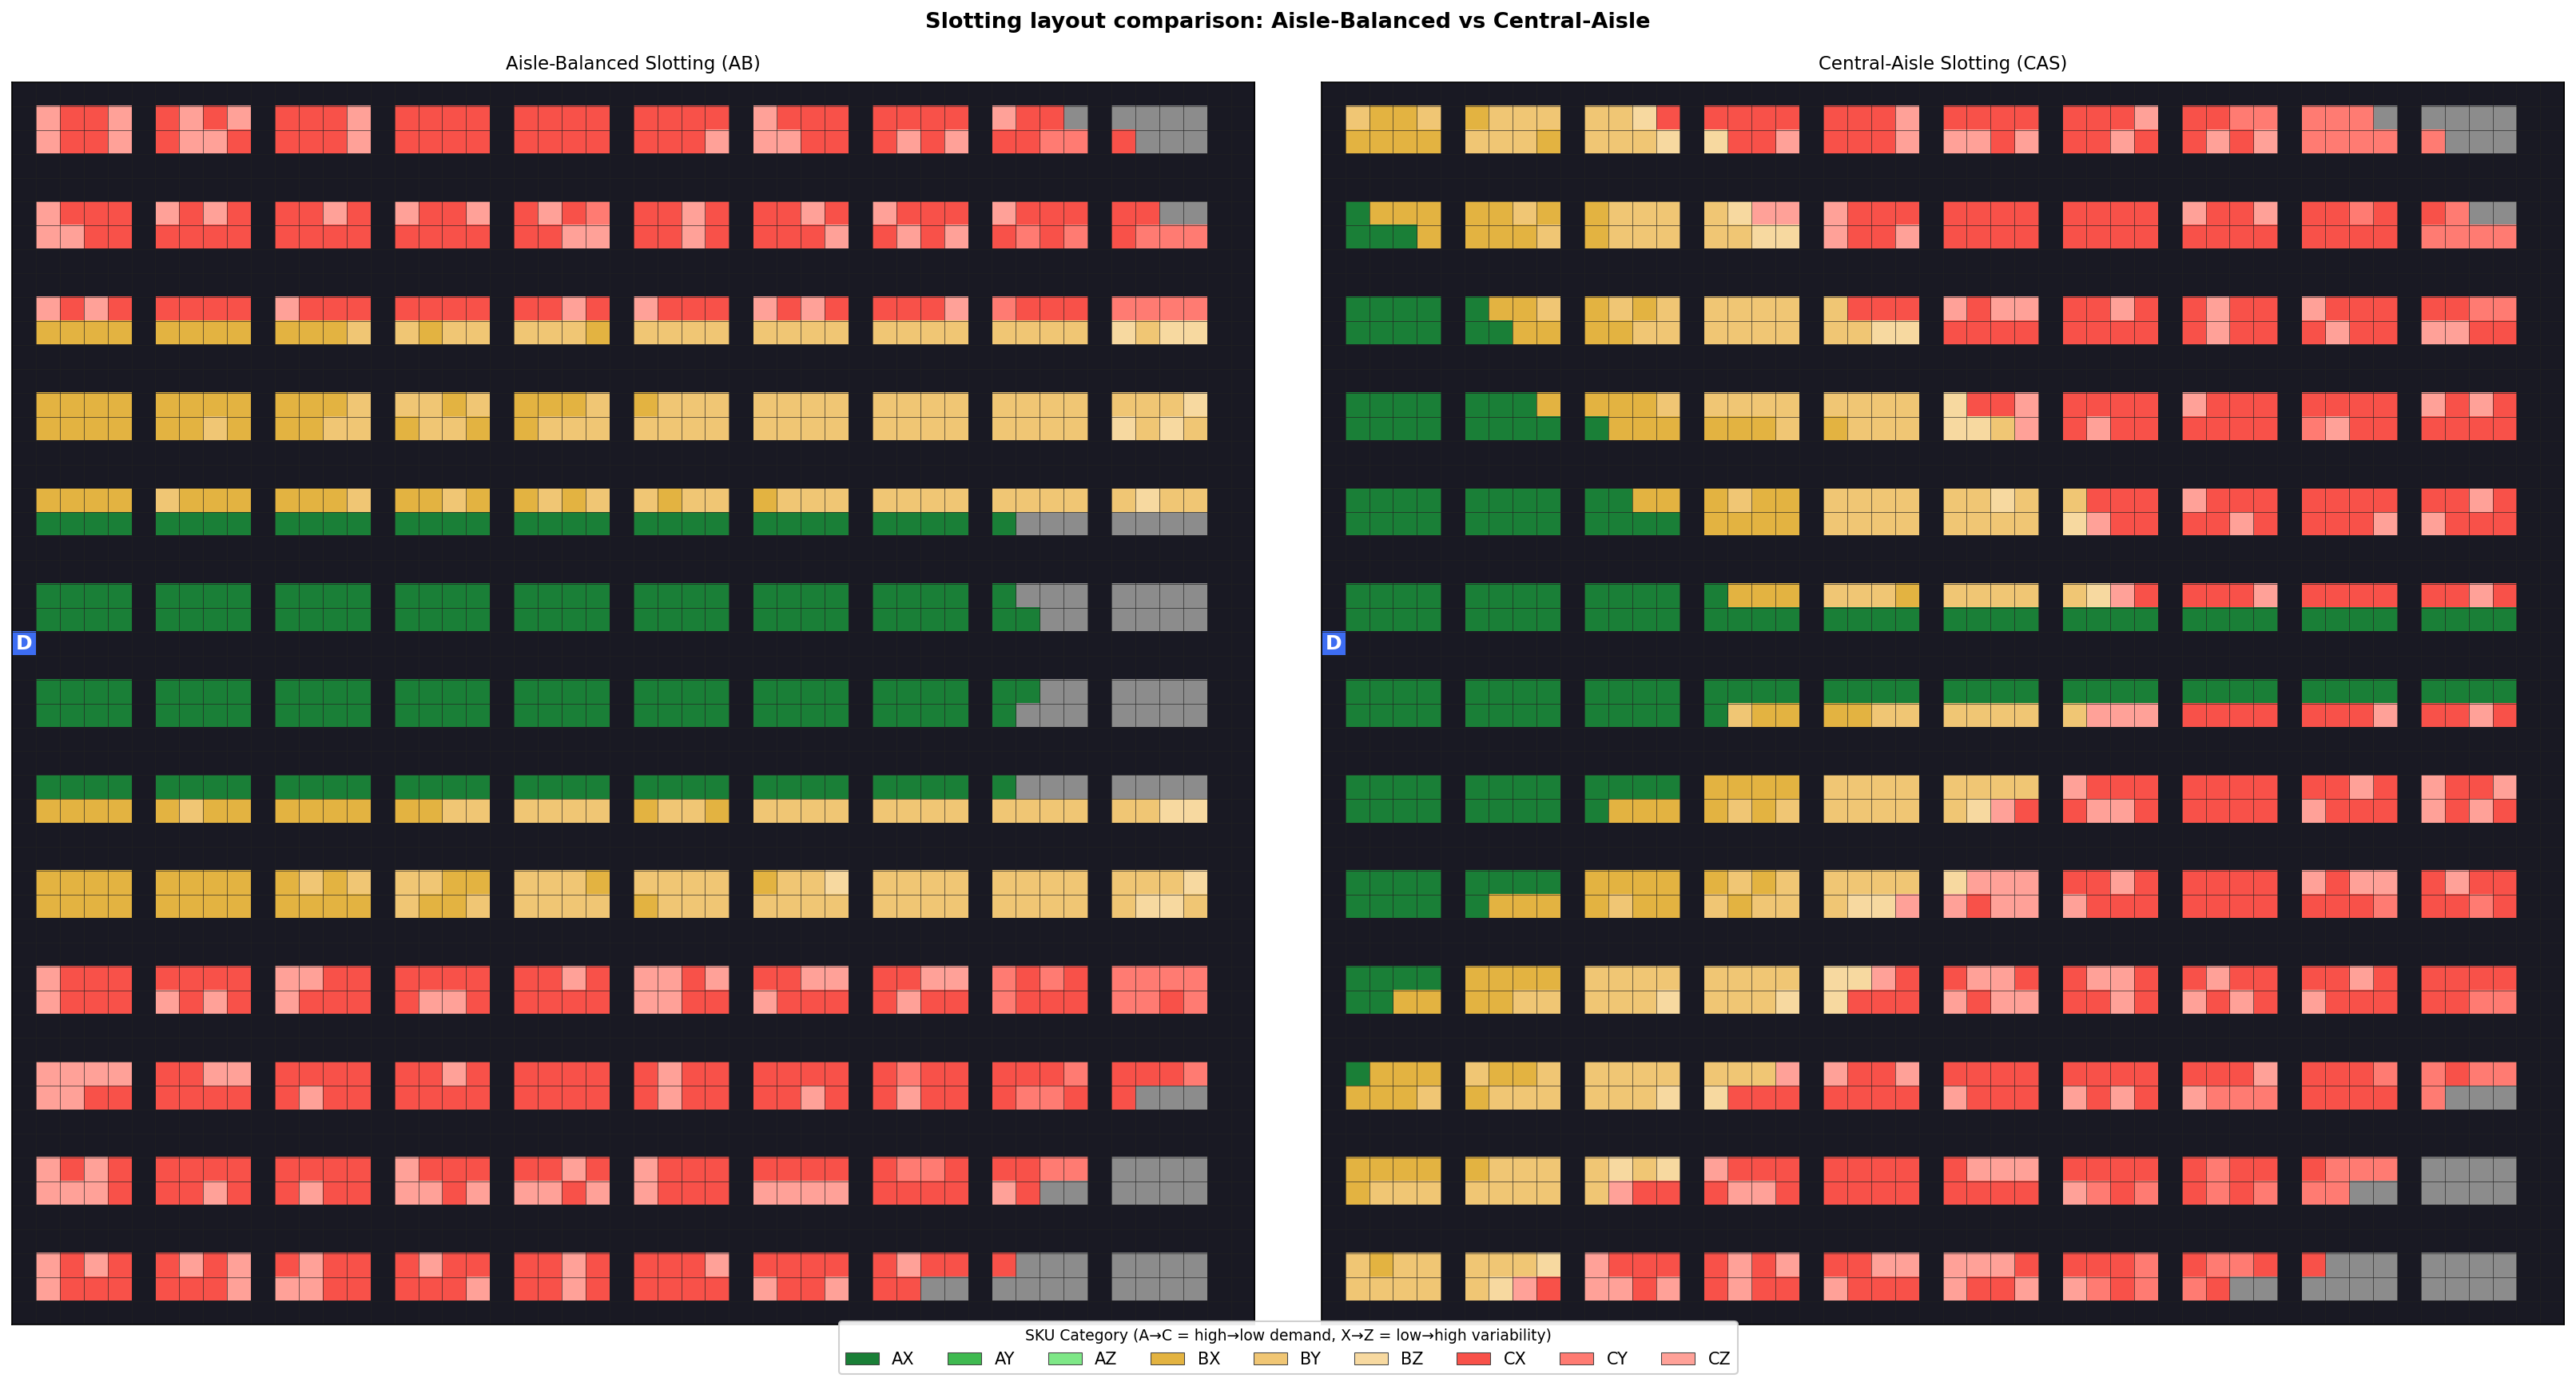
\includegraphics[width=\textwidth]{fig_ab_vs_cas_layout.png}
  \caption{Slotting layouts of Aisle-Balanced (left) and Central-Aisle
    Slotting (right).
    Colour encodes SKU category (AX dark green $\to$ CZ pale red).
    AB spreads A-items across six near-door rows (lateral dispersion);
    CAS stretches the same A-items along the two central rows
    (longitudinal dispersion).}
  \label{fig:ab_vs_cas_layout}
\end{figure}

Figures~\ref{fig:ab_vs_cas_order0} and \ref{fig:ab_vs_cas_typical}
overlay cyan dots on the shelves that hold SKUs from each of the two
representative orders.
For the random order $o_0$ (Figure~\ref{fig:ab_vs_cas_order0}), AB keeps
all $15$ items within a compact cluster close to the door, whereas CAS
stretches them along the central rows; some items land in shelves near
the far right of the warehouse, which is exactly why the $o_0$ route
under CAS grows to $369$~steps.
For the typical order (Figure~\ref{fig:ab_vs_cas_typical}), the picture
is reversed: under CAS the $15$ most demanded SKUs collapse into the
first few columns of the central corridor, so the picker can collect
them in a single short horizontal sweep --- the basis for the $69$-step
route length.
Under AB the same SKUs are distributed across six rows; collecting them
all requires a wider lateral span and the route grows to $107$~steps.

\begin{figure}[H]
  \centering
  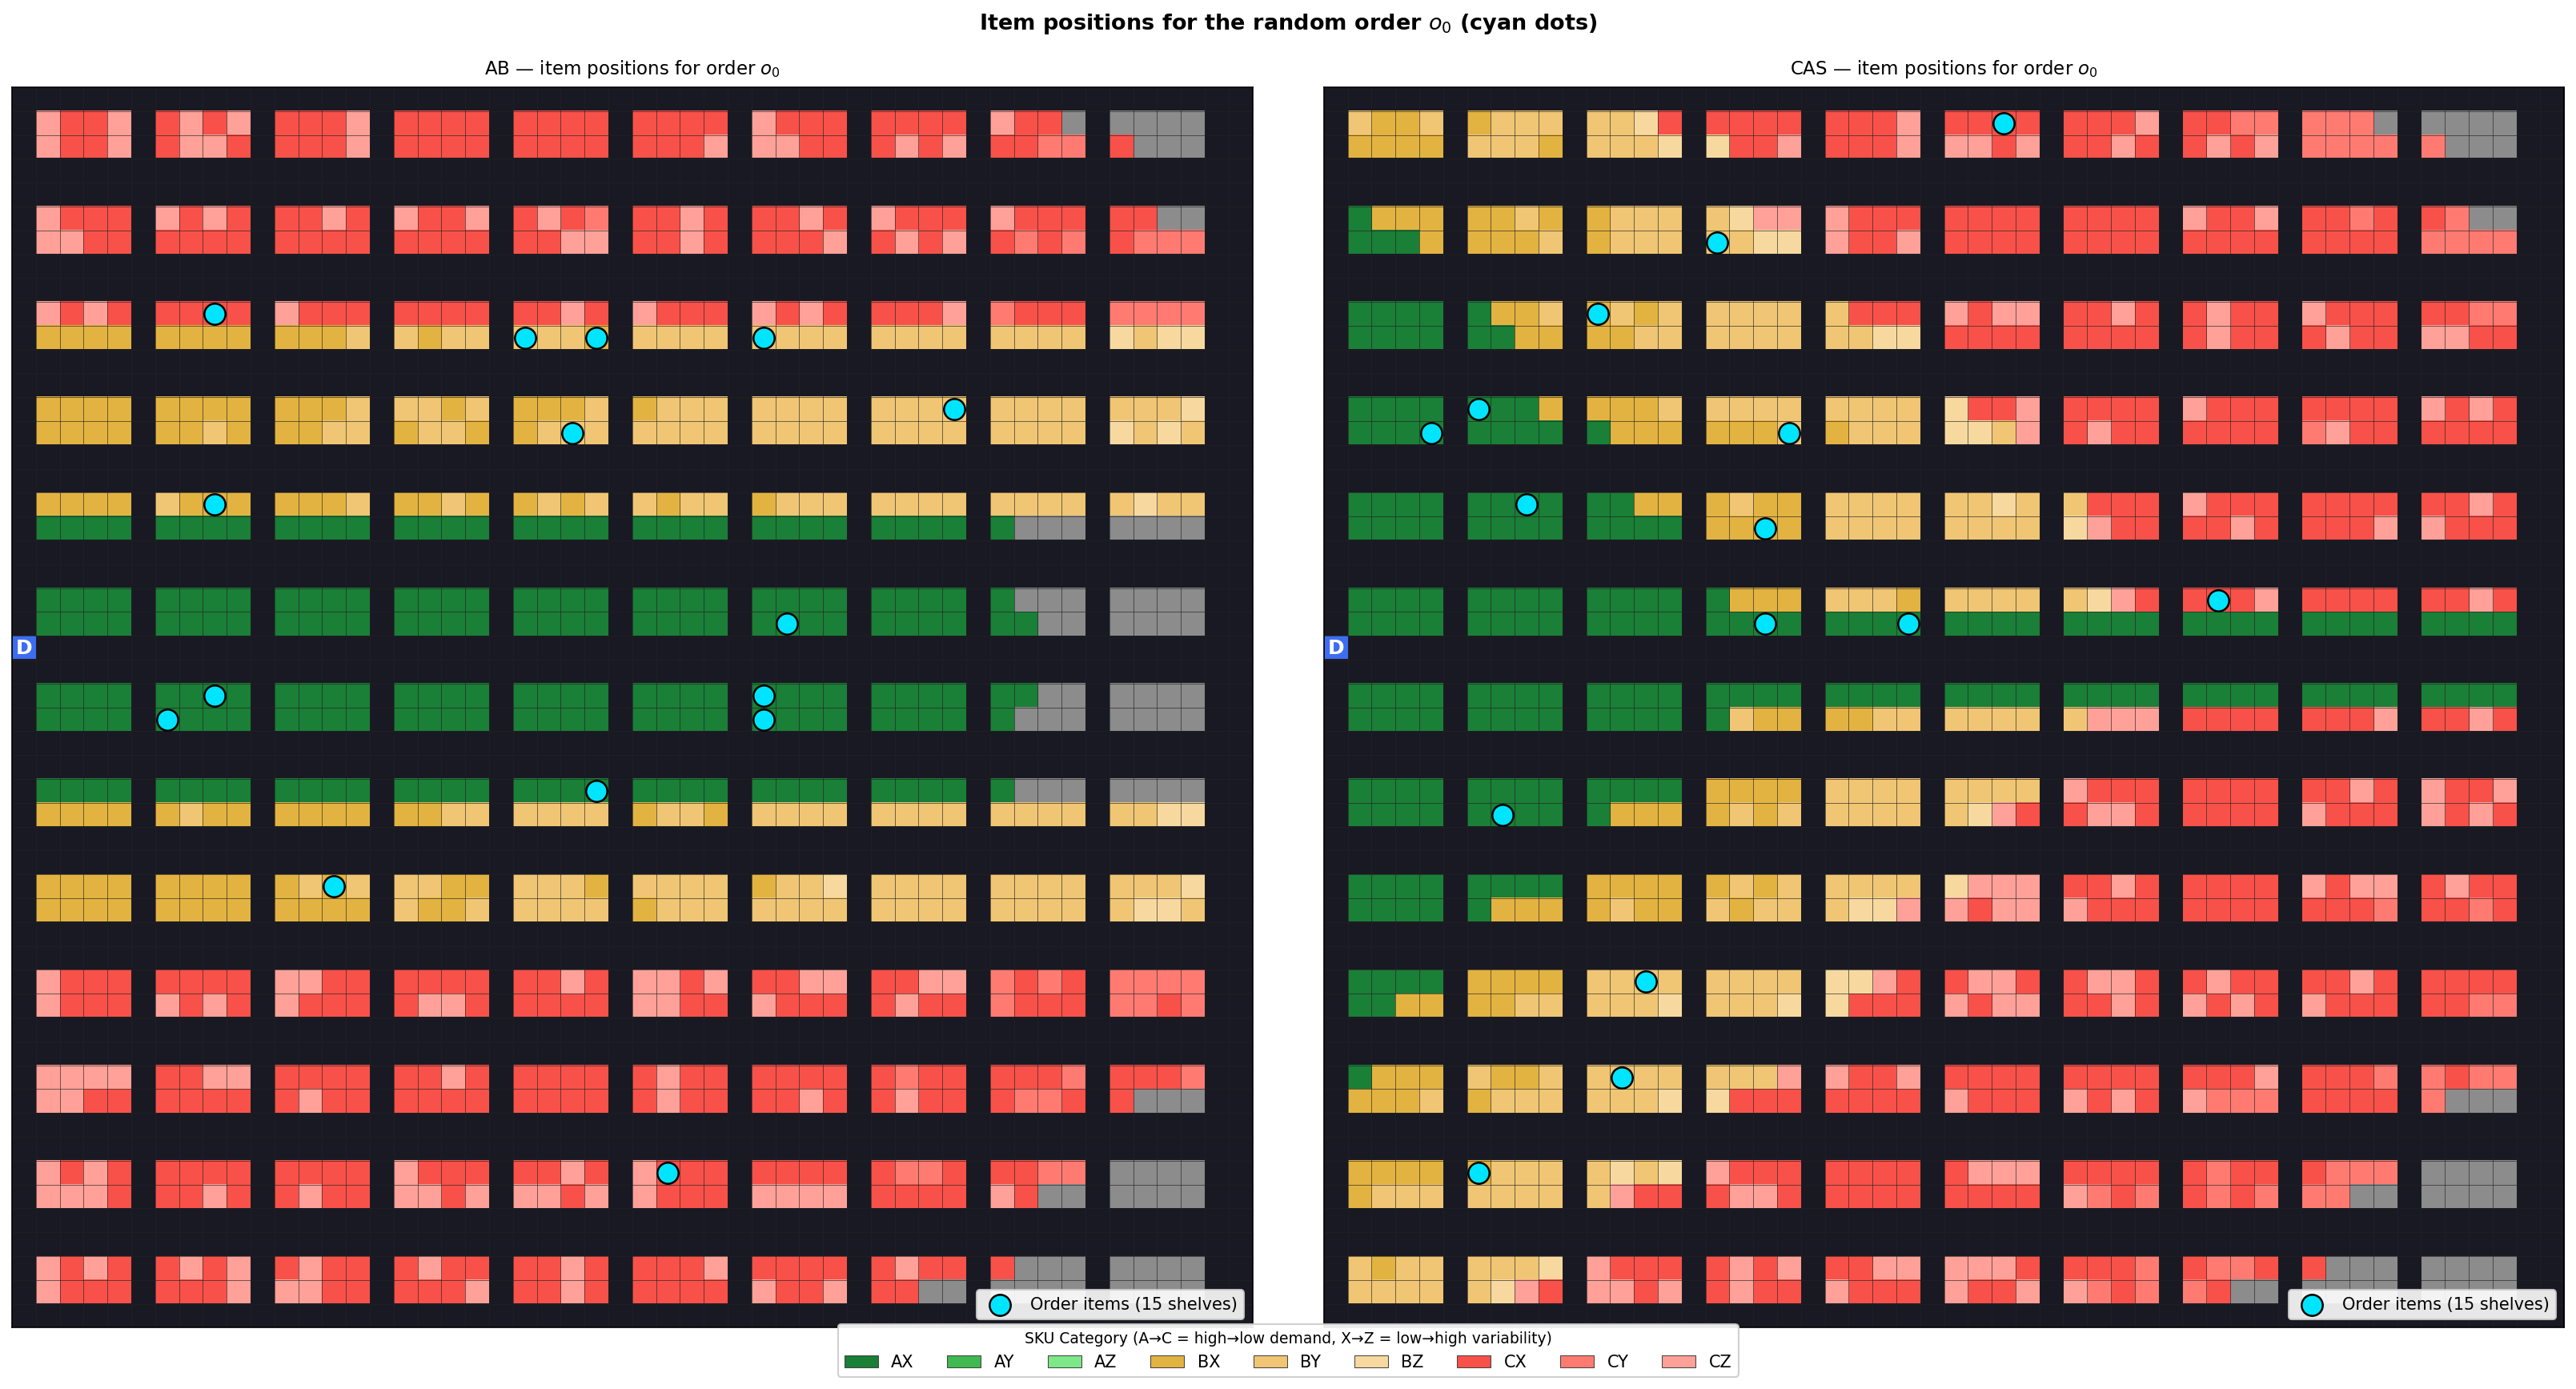
\includegraphics[width=\textwidth]{fig_ab_vs_cas_order0.png}
  \caption{Item positions for the random order $o_0$ under AB (left) and
    CAS (right). Cyan dots mark shelves containing SKUs from the order.
    Under AB the items form a compact cluster near the door; under CAS
    they are stretched along the central horizontal rows, with several
    items in the spilled positions far from the door.}
  \label{fig:ab_vs_cas_order0}
\end{figure}

\begin{figure}[H]
  \centering
  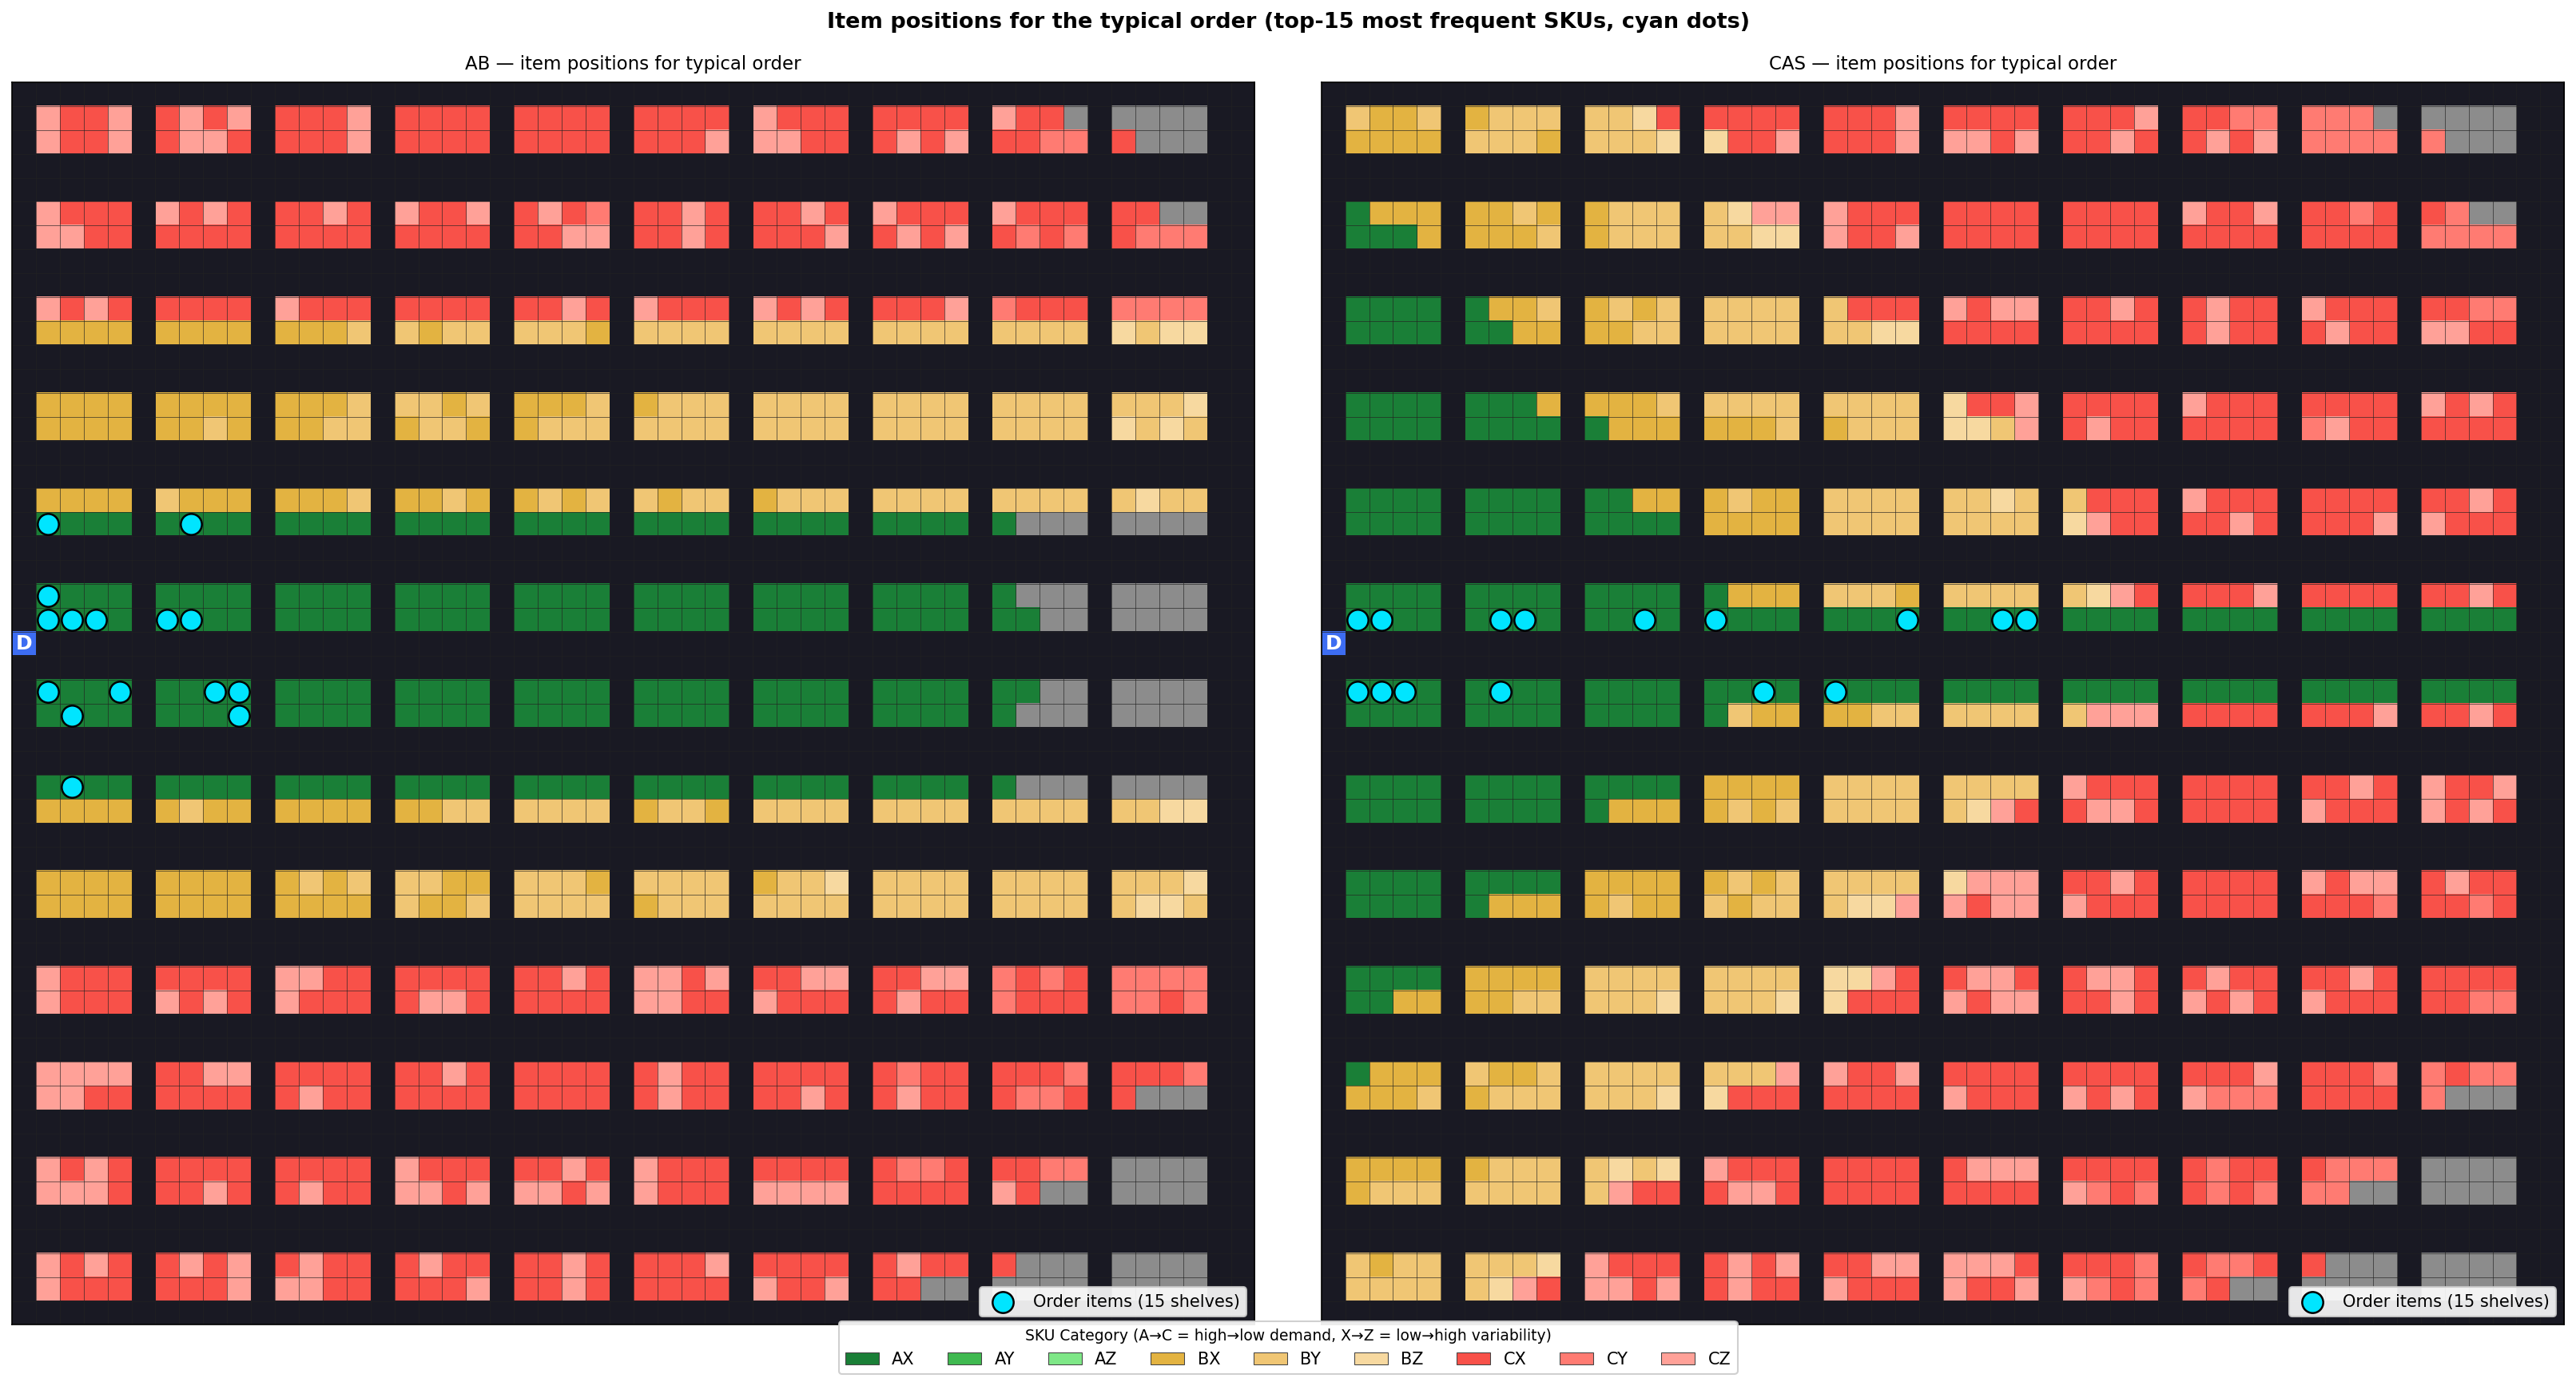
\includegraphics[width=\textwidth]{fig_ab_vs_cas_typical.png}
  \caption{Item positions for the typical order (top-$15$ most frequent
    SKUs) under AB (left) and CAS (right).
    Under AB the items are dispersed across six near-door rows; under CAS
    they collapse into a single tight cluster in the first columns of
    the central corridor, which explains the $69$-step typical-order
    route under CAS.}
  \label{fig:ab_vs_cas_typical}
\end{figure}

The pair of comparisons makes the trade-off behind the table numerical:
CAS specialises the layout for a stable, demand-concentrated order type
(typical) at the cost of less robust performance on broader orders
($o_0$); AB sacrifices a little typical-order performance in exchange for
balanced behaviour across both order types.

\paragraph{Heatmap.}
Figure~\ref{fig:cas_heatmap} shows the traffic heatmap before and after CAS.
The Baseline's focal hot plume at the door is replaced by a long
horizontal band along rows $23$--$24$ extending to the far end of the
warehouse, plus a residual vertical strip near the door from the spilled
A-SKUs in rows $18$--$29$.
The structure of the bottleneck has changed: instead of a single dense
plume immediately in front of the door, CAS produces a thinner but much
longer red band along the central corridor.
The heatmap thus confirms the table's verdict: CAS makes the typical-order
picks dramatically cheaper but does not actually disperse warehouse-wide
traffic --- it just elongates the bottleneck along a different axis.

\begin{figure}[H]
  \centering
  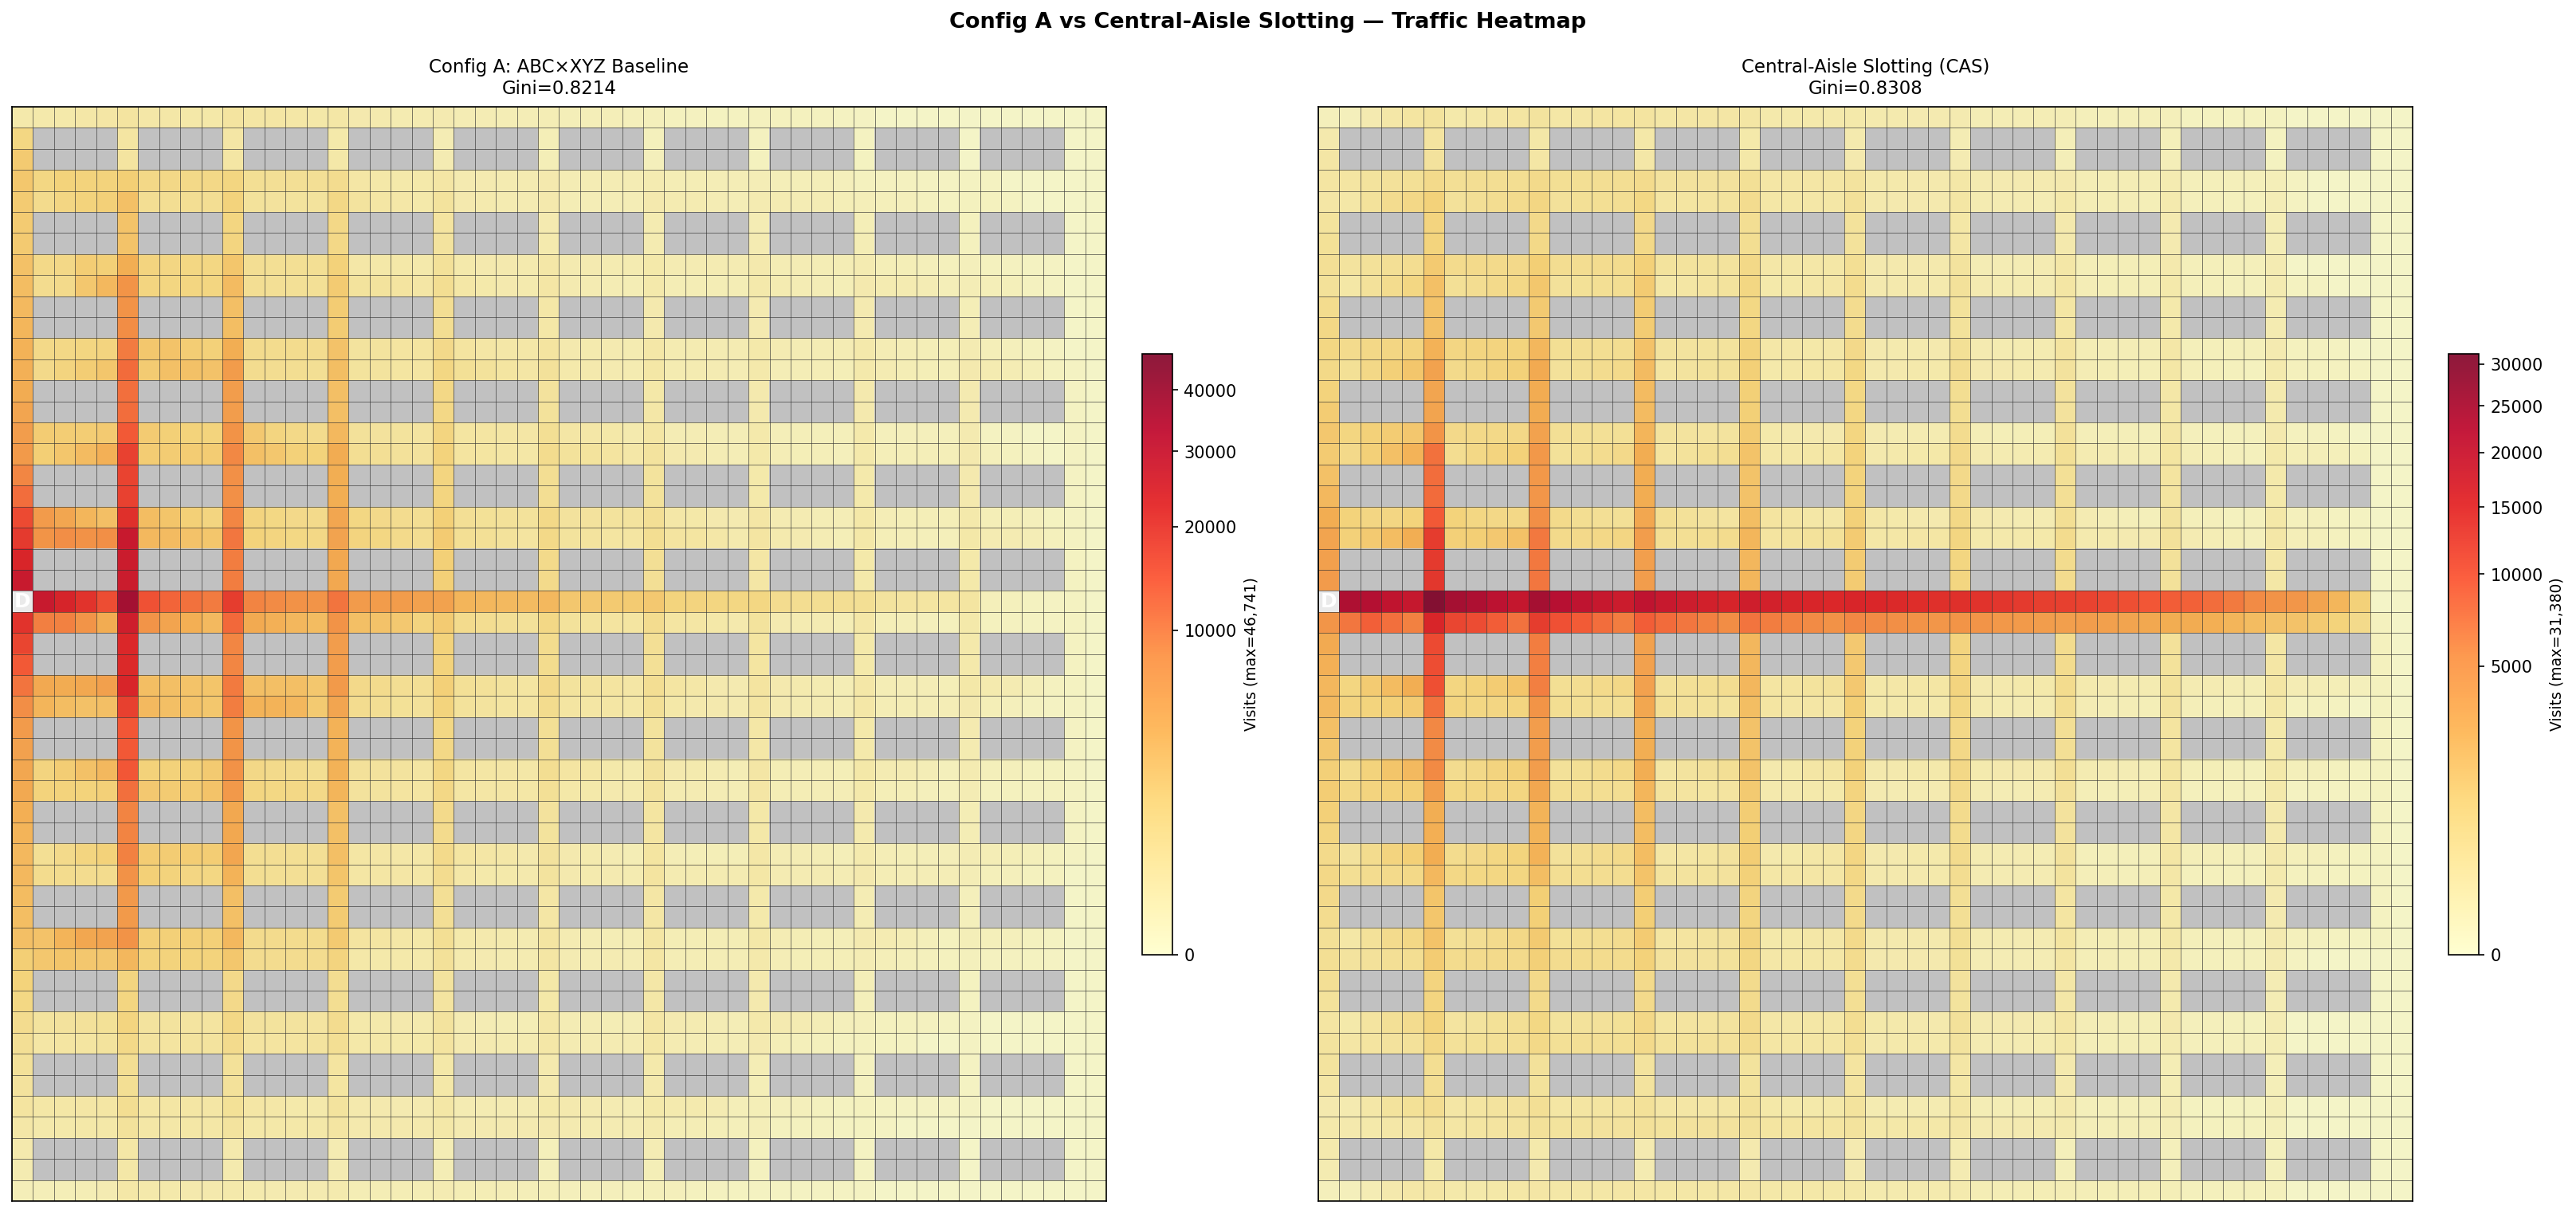
\includegraphics[width=\textwidth]{fig_cas_heatmap.png}
  \caption{Traffic heatmap before (left) and after (right) Central-Aisle
    Slotting.
    The focal entry-corridor plume of the Baseline is replaced by a long
    horizontal band along the door axis;
    Gini is essentially unchanged ($0.672$ vs.\ baseline $0.670$).}
  \label{fig:cas_heatmap}
\end{figure}

\paragraph{Discussion.}
The CAS experiment suggests that single-axis dispersion --- whether
lateral (AB) or longitudinal (CAS) --- can substantially improve
typical-order metrics in the present warehouse layout, and that the
central corridor is an under-used resource in the original
ABC$\times$XYZ placement.
Its weakness is that it concentrates non-typical traffic into a different
single corridor, so the gain on a stable demand profile (heavy A-traffic
dominates) does not transfer to an unpredictable demand profile (random
orders).
Aisle-Balanced, by contrast, sacrifices a few percent of typical-order WPC
to keep \emph{both} order types short, and the Gini stays high precisely
because it intentionally maintains six parallel bands instead of one wide
one.
The choice between CAS and Aisle-Balanced is therefore an explicit
specialisation decision: \textbf{CAS is preferable when the demand mix is
strongly concentrated and stable}; \textbf{Aisle-Balanced is preferable when
the demand mix may shift} or when robustness across order types is
operationally important.
Under demand-unit weighting (A~=~$56.2\%$, B~=~$33.7\%$, C~=~$10.1\%$ order
probability), orders are more diverse than under revenue-weighting, which
partially undermines CAS's specialisation advantage: the spill-zone penalty
becomes more frequent and the typical-order gain ($-47.1\%$ WPC) is smaller
than under a concentrated demand profile.

For the present study, Aisle-Balanced remains the recommended baseline
because it generalises across both representative orders, but CAS provides
a useful upper bound on what is achievable under a fixed-demand
specialisation and confirms that the lateral-concentration diagnosis is
correct: the bottleneck is not about proximity to the door in itself, but
about how A-traffic distributes among the equidistant near-door corridors.

%======================================================================
\section{Config C: Combining Congestion-Aware Routing and Heatmap-Informed Slotting}
%======================================================================

The $2\times2$ experimental design has the routing axis and the slotting
axis as its two intervention points.
Section~9.3.1 measured Config~A (routing axis alone, on the original
ABC$\times$XYZ slotting) and Sections~9.3.2--9.4 measured Config~B (slotting
axis alone, with the simple distance-sort + BFS router).
The remaining quadrant of the $2\times2$ --- \textbf{Config~C}, both axes
active at once --- has not been measured.
This section closes the design.

\subsection{Method}

Config~C is not a new algorithm.
It is the composition of two already-validated components:
\begin{enumerate}
  \item Apply a heatmap-informed slotting to a fresh model
        (e.g.\ Aisle-Balanced or Central-Aisle Slotting).
        The model rebuilds its heatmap on the new placement under BFS
        routing, producing the edge-congestion field $c_e$.
  \item Use the Dijkstra-NN router with $\lambda = 5$ (Section~9.3.1)
        instead of the BFS router.
        Visit-order and path-finding share the cost
        $1 + \lambda c_e$ as in Config~A.
\end{enumerate}
WPC for all Config~C results is measured against the Baseline
ABC$\times$XYZ congestion field $c_e^{\text{base}}$, so the numbers are
directly comparable with all the tables in Section~9.3.

\subsection{Headline result: closing the $2\times2$ design}

Table~\ref{tab:config_c_2x2} closes the $2\times2$ design with CAS as
the slotting choice.
CAS is selected because it gives the strongest typical-order numbers
among the slotting variants (Section~9.4), so the question \emph{``does
adding congestion-aware routing on top buy anything?''} is sharpest there.

\begin{table}[H]
\centering
\caption{The $2\times2$ design closed by Config~C.
  WPC is measured against the Baseline ABC$\times$XYZ congestion field;
  $\Delta$ is the relative change against the Baseline cell.}
\label{tab:config_c_2x2}
\renewcommand{\arraystretch}{1.25}
\begin{tabular}{lcccccc}
\hline
\multirow{2}{*}{\textbf{Cell}} &
  \multicolumn{2}{c}{\textbf{Typ.\ steps}} &
  \multicolumn{2}{c}{\textbf{Typ.\ WPC}} &
  \multirow{2}{*}{\textbf{$o_0$ steps}} &
  \multirow{2}{*}{\textbf{$o_0$ WPC}} \\
 & Value & $\Delta$ & Value & $\Delta$ & & \\
\hline
Baseline (B + BFS)        & 147 & ---       & 55.86 & ---        & 361 & 108.58 \\
Config A (B + Dijkstra-NN) & 85 & $-42.2\%$ & 16.79 & $-69.9\%$ & 249 & 24.89 \\
Config B-CAS (CAS + BFS)   & 69 & $-53.1\%$ & 29.56 & $-47.1\%$ & 369 & 109.15 \\
\textbf{Config C (CAS + Dijkstra-NN)}
                           & \textbf{83} & $\bm{-43.5\%}$ & \textbf{9.15} & $\bm{-83.6\%}$
                           & \textbf{239} & \textbf{23.79} \\
\hline
\end{tabular}
\end{table}

Reading the table.
On the typical order, Config~C achieves the best WPC of all four cells
($9.15$, vs.\ $16.79$ for Config~A and $29.56$ for Config~B-CAS), but its
route length of $83$~steps lies \emph{between} Config~A ($85$~steps) and
Config~B-CAS ($69$~steps).
The Dijkstra-NN router detours around the busy central corridor that CAS
creates, adding a few steps relative to BFS but cutting WPC by $-83.6\%$
vs.\ Baseline.
On the random order~$o_0$, Config~C is the outright winner: $239$~steps
and WPC~$23.79$ --- better than Config~A ($249$ steps, $24.89$ WPC) and
far better than Config~B-CAS ($369$ steps, $109.15$ WPC).
Config~C therefore simultaneously dominates all alternatives on $o_0$ and
leads on typical WPC, at a modest cost of $14$~extra steps on the typical
route relative to Config~B-CAS.

\paragraph{Composition: closer to multiplicative than additive.}
A naive expectation might be that the gains of routing and slotting
\emph{add}: Config~A gives $-69.9\%$ typical WPC and Config~B-CAS gives
$-47.1\%$. Adding these is not operationally meaningful, since the sum
exceeds $100\%$. A multiplicative model is more consistent with the data:
$(1 - 0.699) \times (1 - 0.471) = 0.159$, which corresponds to a reduction
of $-84.1\%$ from the Baseline, close to the observed $-83.6\%$.
This suggests that slotting and routing act on different parts of the
WPC product: the slotting reduces the average $c_e$ along the shortest
path (placing items in cooler corridors), while routing further reduces
the path's contact with the hot edges that remain.
The single data point does not prove the multiplicative form, but it is
consistent with it.

\subsection{Extending the menu: all seven slottings under Dijkstra-NN}

Table~\ref{tab:config_c_matrix} reports the full $7 \times 2$ matrix:
each of the seven slottings of Section~9.3 evaluated under both BFS and
Dijkstra-NN routing.
The CA column is the Config~C generalisation.

\begin{table}[H]
\centering
\caption{Full $7 \times 2$ matrix of slottings under BFS and Dijkstra-NN routing
  ($\lambda = 5$). WPC against $c_e^{\text{base}}$; $K = 10\,000$ orders, seed $42$.
  $L_{95}$ is the 95th percentile of per-order route length over all $K$ orders.
  Best non-CAS Config~C cell highlighted in bold; CAS Config~C numbers in
  bold-italic.}
\label{tab:config_c_matrix}
\renewcommand{\arraystretch}{1.15}
\setlength{\tabcolsep}{3pt}
\begin{tabular}{l|ccccc|ccccc}
\hline
\multirow{2}{*}{\textbf{Slotting}} &
  \multicolumn{5}{c|}{\textbf{BFS routing}} &
  \multicolumn{5}{c}{\textbf{Dijkstra-NN routing (Config~C)}} \\
 & typ\,st & typ\,WPC & $o_0$\,st & $o_0$\,WPC & $L_{95}$
 & typ\,st & typ\,WPC & $o_0$\,st & $o_0$\,WPC & $L_{95}$ \\
\hline
Baseline (ABC$\times$XYZ) & 147 & 55.86 & 361 & 108.58 & 439 &  85 & 16.79 & 249 & 24.89 & 281 \\
DWC ($\Delta = 5$)         & 147 & 55.86 & 361 & 108.58 & 439 &  85 & 16.79 & 249 & 24.89 & 281 \\
HZR ($h = 0.15$)           & 389 & 28.20 & 513 &  67.12 & 559 & 255 & 13.29 & 283 & 26.26 & 335 \\
TAPS ($\alpha = 3$)        & 111 & 50.82 & 377 & 118.50 & 443 &  75 & 15.75 & 233 & 29.31 & 275 \\
\textbf{Aisle-Balanced}    & 107 & 46.25 & 353 &  83.37 & 371
                           & \textbf{63} & \textbf{10.62} & \textbf{263} & \textbf{28.73} & 273 \\
AAHMS ($K = 150$)          & 115 & 46.00 & 353 &  83.37 & 373 & 111 & 18.81 & 263 & 28.73 & \textbf{271} \\
CAS                        &  69 & 29.56 & 369 & 109.15 & 435
                           & \textit{\textbf{83}} & \textit{\textbf{9.15}}
                           & \textit{\textbf{239}} & \textit{\textbf{23.79}}
                           & \textit{\textbf{279}} \\
\hline
\end{tabular}
\end{table}

Several patterns emerge from the matrix.
\emph{First}, for most slottings, replacing BFS with Dijkstra-NN shortens
the typical route considerably: Baseline/DWC drop from $147$ to $85$~steps
($-42\%$), Aisle-Balanced from $107$ to $63$ ($-41\%$), TAPS from $111$
to $75$ ($-32\%$), and HZR from $389$ to $255$ ($-34\%$). Two exceptions
are worth noting: AAHMS shortens only marginally ($115 \to 111$, $-3.5\%$),
and CAS actually \emph{lengthens} the typical route from $69$ to $83$ steps
($+20\%$) because the router trades extra steps for lower WPC. In both
exceptions WPC still decreases substantially.
\emph{Second}, Dijkstra-NN reduces WPC compared to BFS on every tested
slotting, even when BFS WPC was already low. The smallest relative
reduction is on HZR ($28.20 \to 13.29$, $-53\%$), where
the slotting already dispersed hot traffic; CAS ($29.56 \to 9.15$,
$-69\%$) and Baseline/DWC ($55.86 \to 16.79$, $-70\%$) show
comparable relative gains.
\emph{Third}, the best Config~C cell on typical steps is \textbf{Aisle-Balanced~+~CA}
($63$~steps), while the best on typical WPC is \textbf{CAS~+~CA} ($9.15$).
On $o_0$, the picture is split: CAS~+~CA gives the lowest WPC
($23.79$, against the next-best $24.89$ for Config~A), while
\textbf{TAPS~+~CA} gives the shortest route ($233$~steps, against
$239$ for CAS~+~CA).
\emph{Fourth}, the $L_{95}$ column confirms the robustness pattern.
Under BFS routing, $L_{95}$ ranges from $371$ (AB) to $559$ (HZR),
with HZR being a clear outlier because $164\%$ longer typical routes
inflate the upper tail of the distribution.
Under Dijkstra-NN, $L_{95}$ falls into a much tighter range of
$271$--$335$~steps, with AAHMS~+~CA giving the lowest tail
($271$~steps) closely followed by AB~+~CA ($273$) and TAPS~+~CA
($275$). The differences between AAHMS, AB, TAPS, and CAS within
Config~C are small (within $8$~steps at the $95$-th percentile),
which means that for routine pickers all four candidates produce
similarly bounded worst-case routes. HZR stays the outlier at
$335$~steps, $20\%$ above the next-worst configuration, reinforcing
its exclusion on operational grounds.

\subsection{\texorpdfstring{$\lambda$}{lambda}-sensitivity under CAS}

The $\lambda$-sweep in Section~9.3.1 was performed on the Baseline
ABC$\times$XYZ layout.
Under CAS the hot zone has a different shape (a long horizontal band
rather than a focal plume), so the operating point of the
congestion penalty may shift.
Table~\ref{tab:config_c_lambda_cas} reports the sweep on CAS at
$\lambda \in \{0, 1, 2, 5, 10, 20\}$.

\begin{table}[H]
\centering
\caption{$\lambda$-sensitivity of Dijkstra-NN on the CAS layout
  ($K = 10\,000$ orders, seed $42$; WPC against $c_e^{\text{base}}$).
  Bold marks the column-wise best; $\mathbf{5}$ is the chosen operating point.}
\label{tab:config_c_lambda_cas}
\renewcommand{\arraystretch}{1.20}
\begin{tabular}{ccccccccc}
\hline
$\lambda$ & typ\,steps & typ\,WPC & $o_0$\,steps & $o_0$\,WPC
          & mean\,steps & $L_{95}$ & mean\,WPC & Gini \\
\hline
$0$  &  \textbf{69} & 29.56 & 369 & 109.15 & 336.3 & 435 & 102.52 & 0.672 \\
$1$  &  \textbf{69} & 11.74 & 221 &  30.45 & \textbf{222.3} & \textbf{275} & 28.56 & 0.672 \\
$2$  &  73 &  9.37 & \textbf{211} &  34.54 & 224.1 & \textbf{275} & 26.38 & 0.672 \\
$\mathbf{5}$ & 83 & 9.15 & 239 & 23.79 & 228.6 & 279 & 23.88 & 0.672 \\
$10$ & 89 & \textbf{8.67} & 265 & 30.13 & 236.8 & 289 & 22.30 & 0.672 \\
$20$ & 89 & \textbf{8.67} & 305 & \textbf{22.22} & 262.7 & 337 & \textbf{20.74} & 0.672 \\
\hline
\end{tabular}
\end{table}

The sweep on CAS under demand-unit weighting shows a different pattern from the
revenue-weighted setup.
At $\lambda = 0$ the CAS + BFS route is $69$~steps with WPC~$29.56$.
At $\lambda = 1$ WPC drops sharply to $11.74$ while steps stay at $69$;
at $\lambda = 2$ the route grows slightly to $73$~steps but WPC reaches $9.37$.
The $\lambda = 5$ result from the $7 \times 2$ matrix gives $83$~steps
and WPC~$9.15$ --- slightly longer route but lower WPC than $\lambda = 2$.
Extending to $\lambda = 10$ and $\lambda = 20$, the typical-order WPC
reaches its floor at $8.67$ (tied), while route length grows to $89$~steps
and mean route length increases from $228.6$ to $236.8$ and $262.7$~steps
respectively.
The $o_0$ column improves dramatically from $369$ steps at $\lambda = 0$ to
$211$~steps at $\lambda = 2$, then recovers to $265$ and $305$~steps at
$\lambda = 10$ and $\lambda = 20$, suggesting that the CA router is highly
effective at routing around the central hot band at moderate $\lambda$.

The chosen value $\lambda = 5$ used throughout Config~C is consistent with the
validated Baseline setting and offers a good WPC reduction ($-83.6\%$) with
acceptable route length.
A production deployment of CAS + Dijkstra-NN would benefit from a re-tune
around $\lambda \approx 1$--$2$ for minimum route length ($222$--$224$~steps mean),
or $\lambda \approx 10$--$20$ for minimum WPC ($8.67$, at the cost of
mean routes of $237$--$263$~steps).

\subsection{Practical winner: Aisle-Balanced + Dijkstra-NN}

Under demand-unit weighting, AB~+~CA offers the best balance across all
metrics: shortest typical route, best mean route length, and competitive
WPC on both order types.
CAS~+~CA achieves the lowest typical-order WPC ($9.15$) but pays a penalty
on typical steps ($83$ vs.\ $63$) relative to AB~+~CA:

\begin{itemize}
  \item Typical order: AB + CA gives $63$ steps and WPC $10.62$, within
        $20$~steps of CAS~+~CA but $8$~steps shorter;
  \item Order $o_0$: CAS + CA gives $239$ steps and WPC $23.79$;
        the WPC is the best value across the whole $7 \times 2$ matrix,
        while the route length is second-best (the shortest $o_0$ route
        in the matrix is TAPS~+~CA with $233$~steps);
  \item Mean batch route length: AB + CA gives $211.2$ steps, lower than
        any other configuration measured ($228.6$ for CAS~+~CA).
\end{itemize}

The recommended configuration for the present warehouse is therefore
\textbf{Aisle-Balanced slotting combined with Dijkstra-NN routing
($\lambda = 5$)}.
CAS + CA is retained in the design space as the upper bound on typical-order
WPC under demand-stable specialisation.

\subsection{Visual evidence}

\paragraph{Bar-chart summary.}
Figure~\ref{fig:config_c_summary} consolidates the four cells of
Table~\ref{tab:config_c_2x2} into bar charts.
The Config~C bar is the only one that simultaneously sits at or near
the minimum of every panel.

\begin{figure}[H]
  \centering
  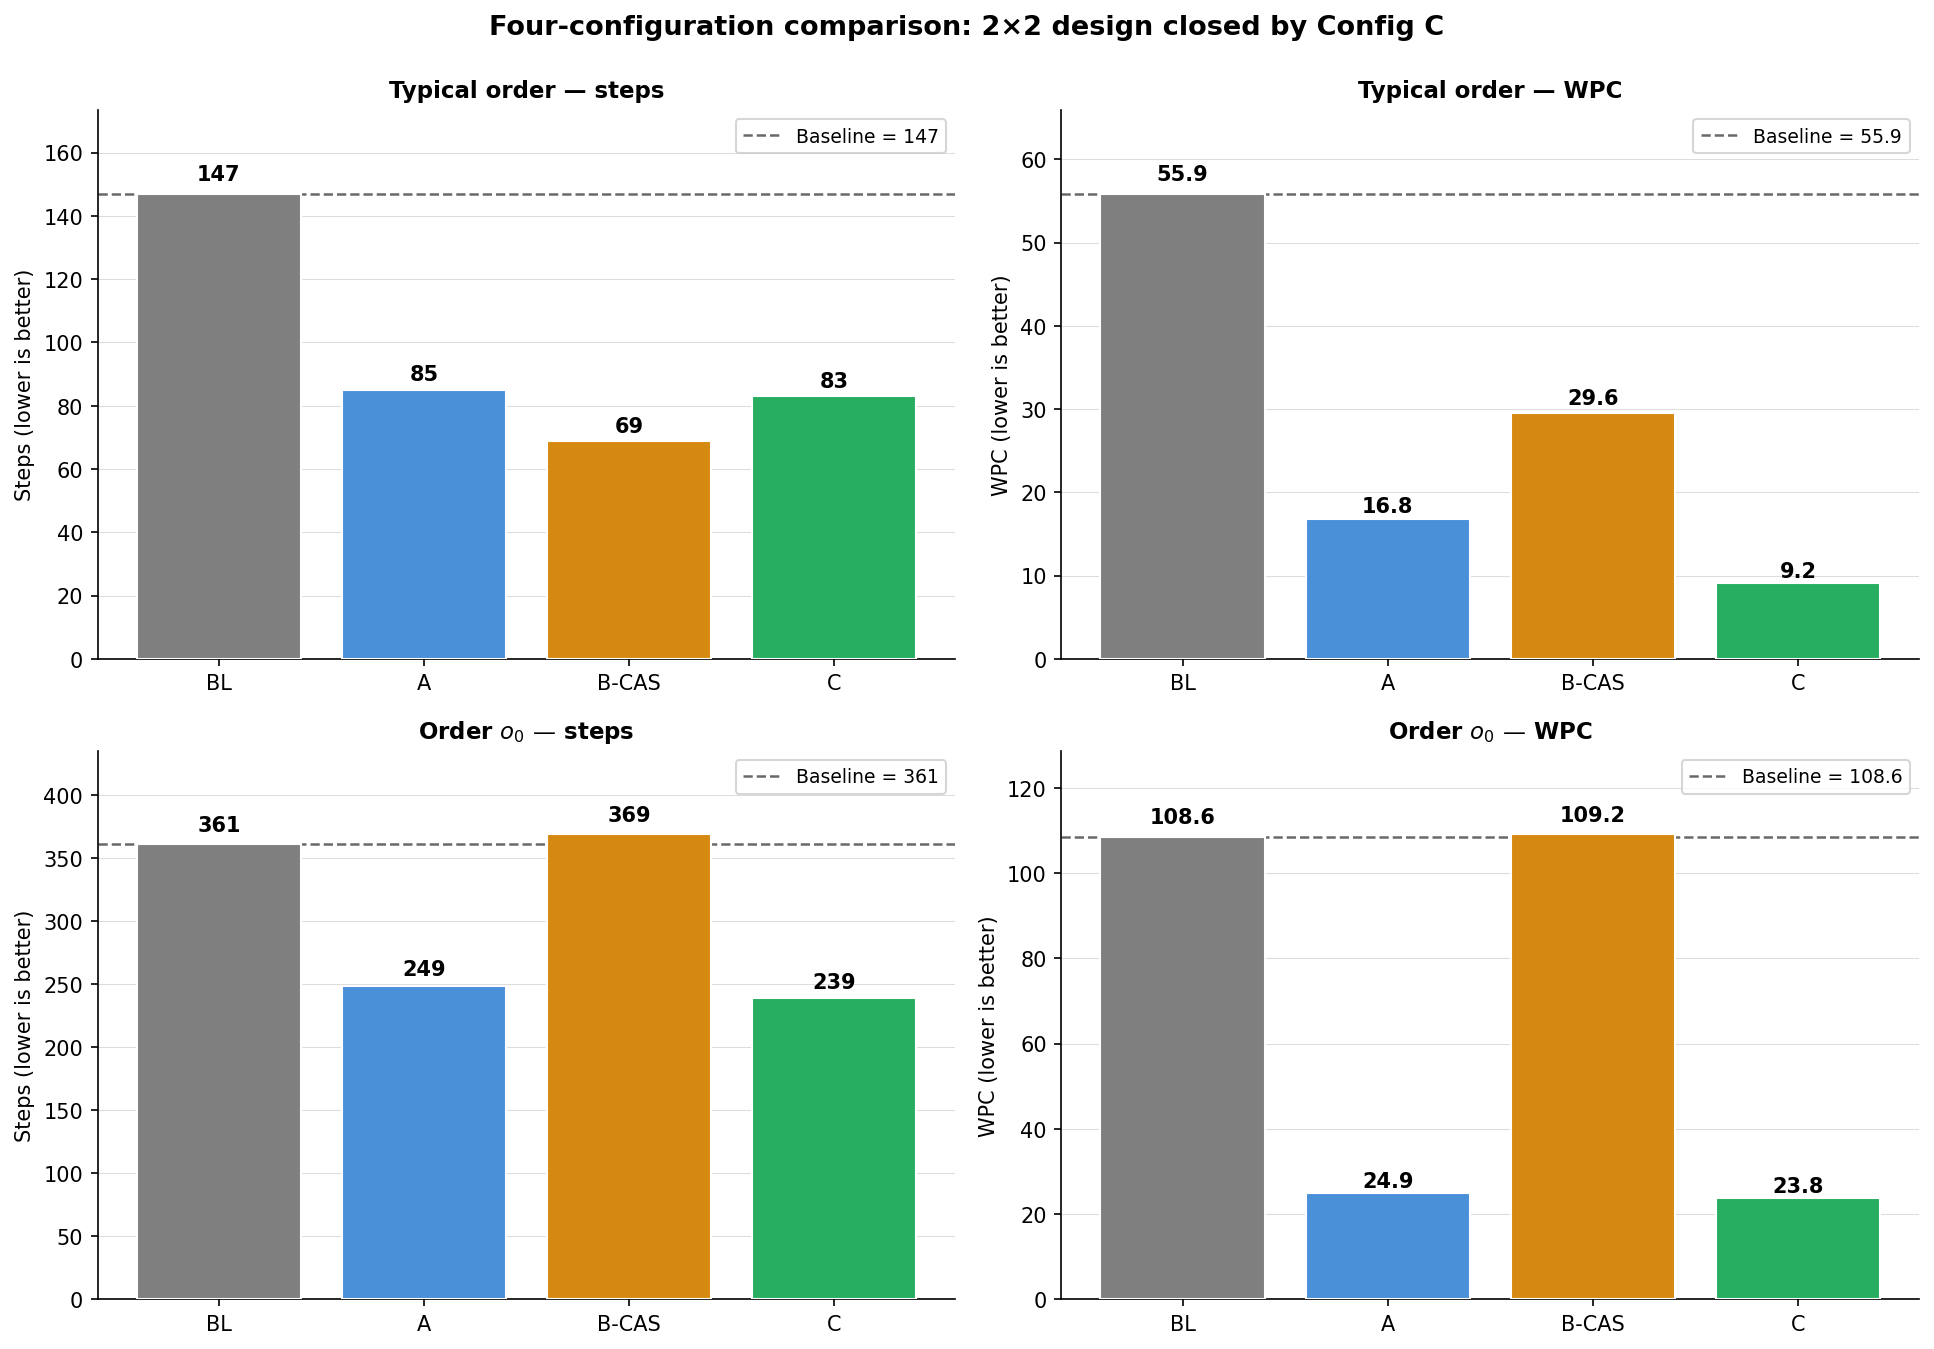
\includegraphics[width=0.90\textwidth]{fig_config_c_summary.png}
  \caption{Four-configuration comparison.
    Bars: Baseline (grey), Config~A (blue), Config B-CAS (orange),
    Config~C (green).
    Dashed lines show the Baseline value for each metric.
    Config~C wins typical-order metrics and matches or beats the
    Baseline on $o_0$.}
  \label{fig:config_c_summary}
\end{figure}

\paragraph{Recommended configuration: AB + Dijkstra-NN.}
Figure~\ref{fig:ab_routes} shows the picking routes on the
Aisle-Balanced layout, which corresponds to the recommended Config~C
cell.
On the typical order (bottom row), BFS already finds a short
$107$-step route across six near-door rows; Dijkstra-NN further
reduces it to $63$~steps by collecting all $15$ items in a tight
out-and-back sweep along the rows immediately around the door.
On $o_0$ (top row), the BFS route grows to $353$~steps because the
items are spread across the warehouse; Dijkstra-NN cuts the route to
$263$~steps by reordering the visits and detouring around the busiest
corridors.

\begin{figure}[H]
  \centering
  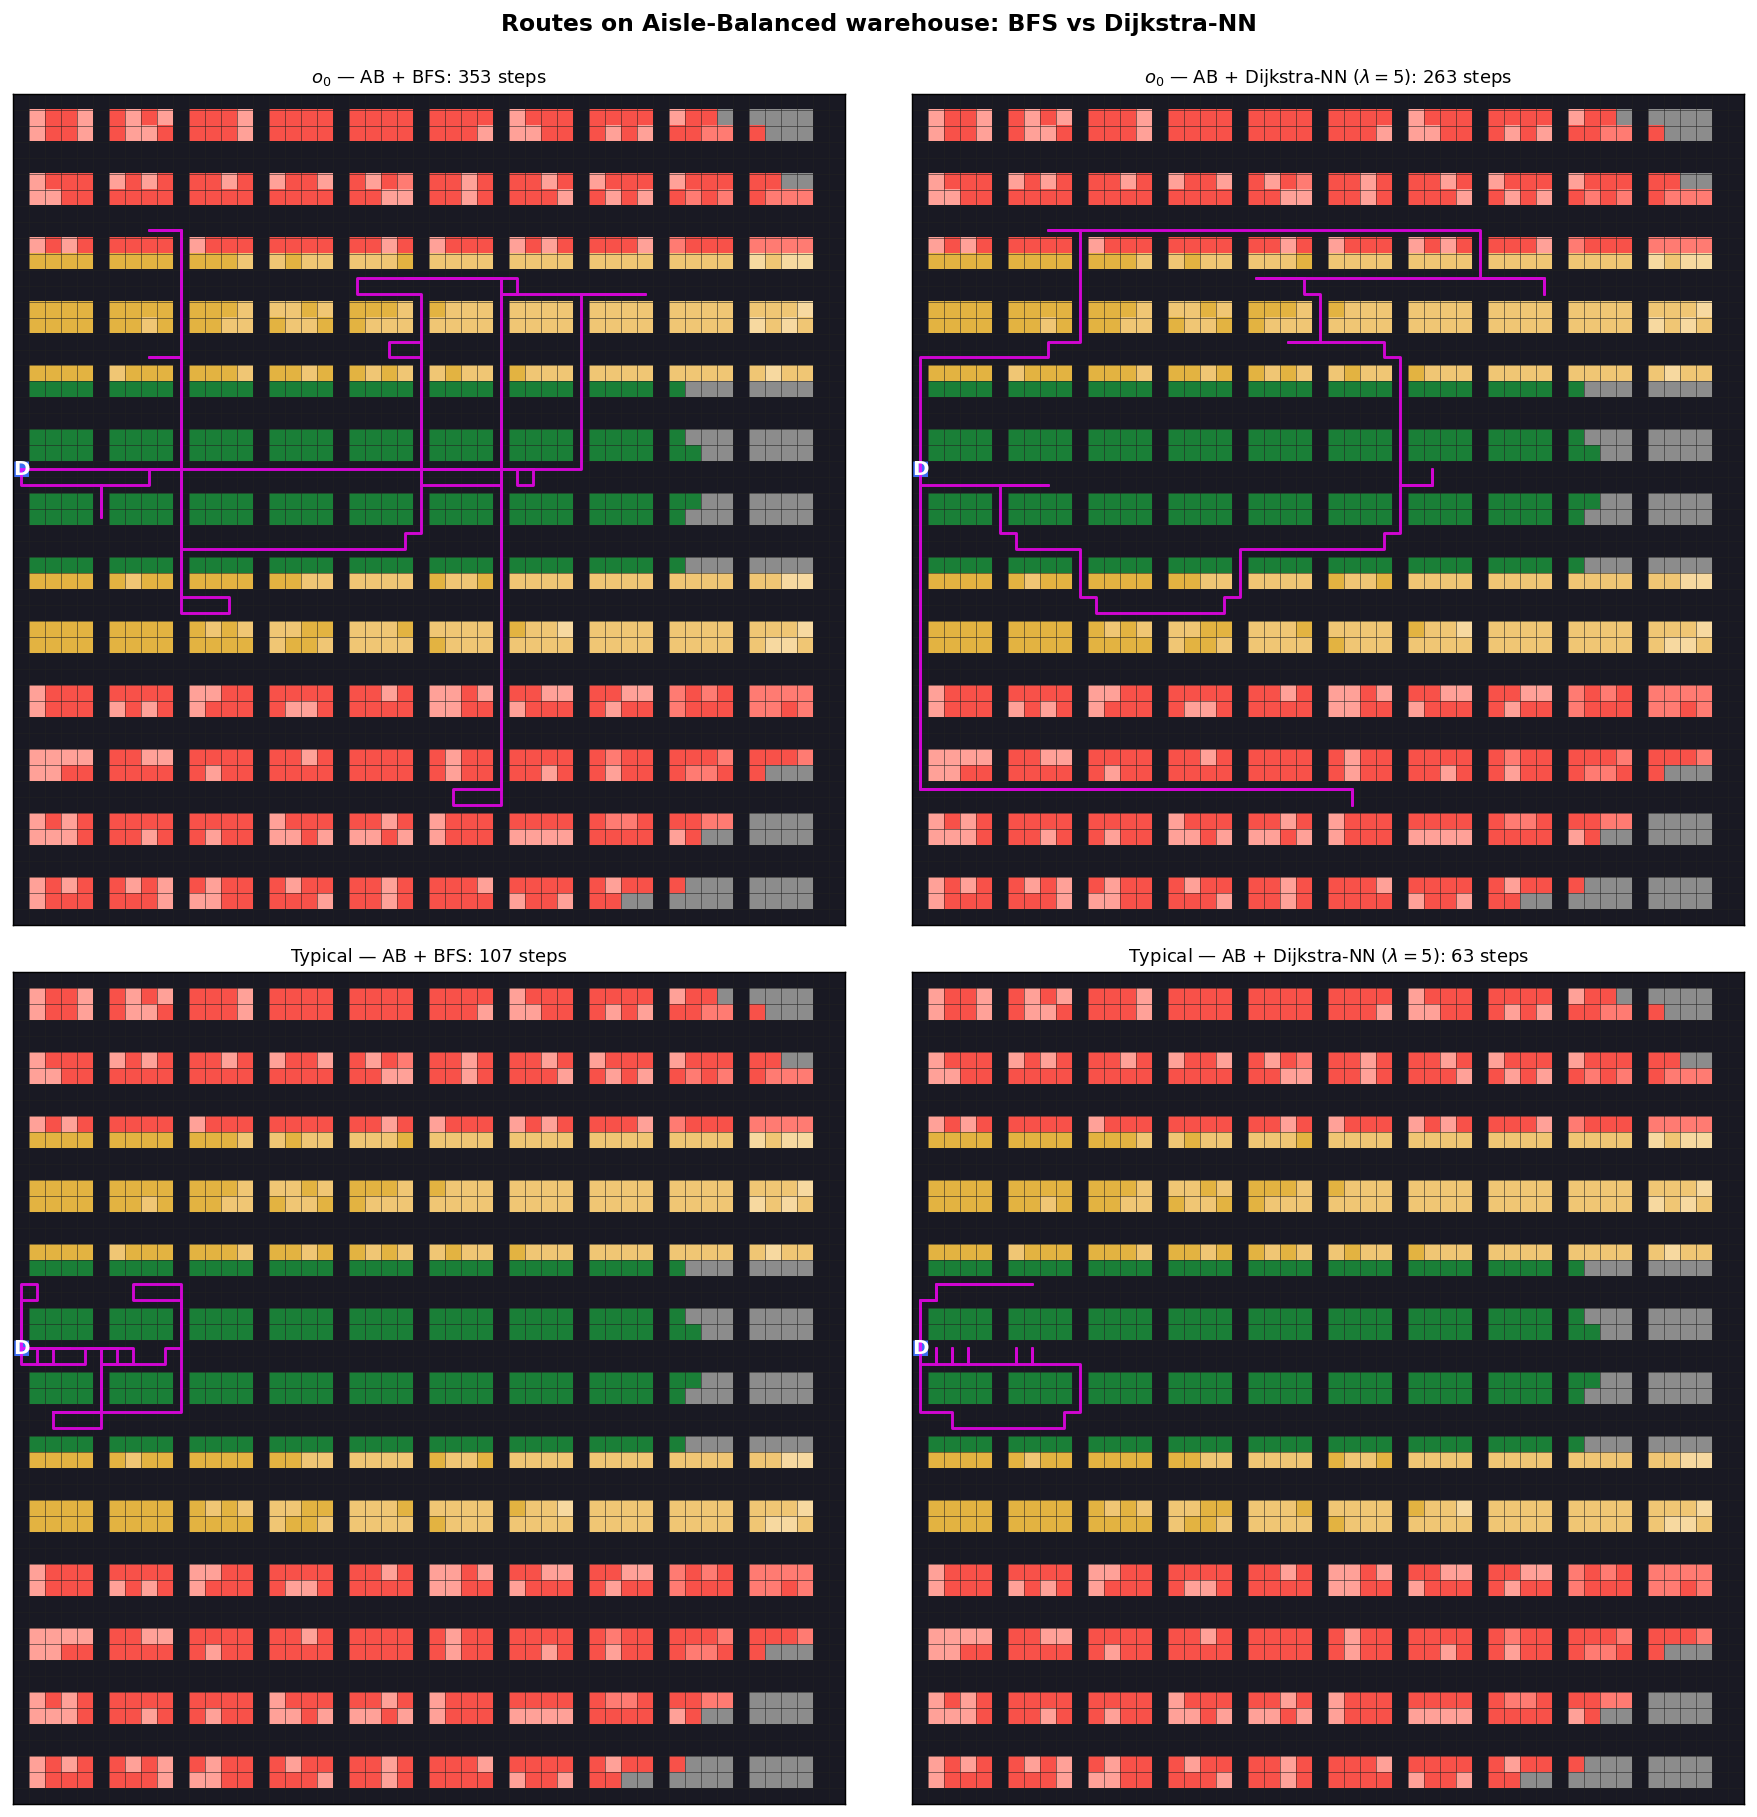
\includegraphics[width=\textwidth]{fig_ab_routes.png}
  \caption{Routes on the Aisle-Balanced warehouse (recommended Config~C).
    Rows: order $o_0$ (random) above; typical order below.
    Columns: BFS routing (left); Dijkstra-NN $\lambda = 5$ (right).
    Magenta = picking path; D = door.
    Dijkstra-NN shortens both routes on the AB layout: $107 \to 63$
    on the typical order and $353 \to 263$ on $o_0$.}
  \label{fig:ab_routes}
\end{figure}

\paragraph{Specialised configuration: CAS + Dijkstra-NN.}
For comparison, Figure~\ref{fig:config_c_routes} shows the same routes
on the CAS layout, the specialised alternative.
On the typical order, CAS + BFS already produces a very short
$69$-step horizontal sweep;
Dijkstra-NN lengthens it slightly to $83$~steps but cuts WPC from
$29.56$ to $9.15$ by routing through cells with lower baseline
congestion weights.
On $o_0$, Dijkstra-NN substantially reduces the spill detour,
bringing route length from $369$ to $239$~steps and WPC from $109.15$
to $23.79$.

\begin{figure}[H]
  \centering
  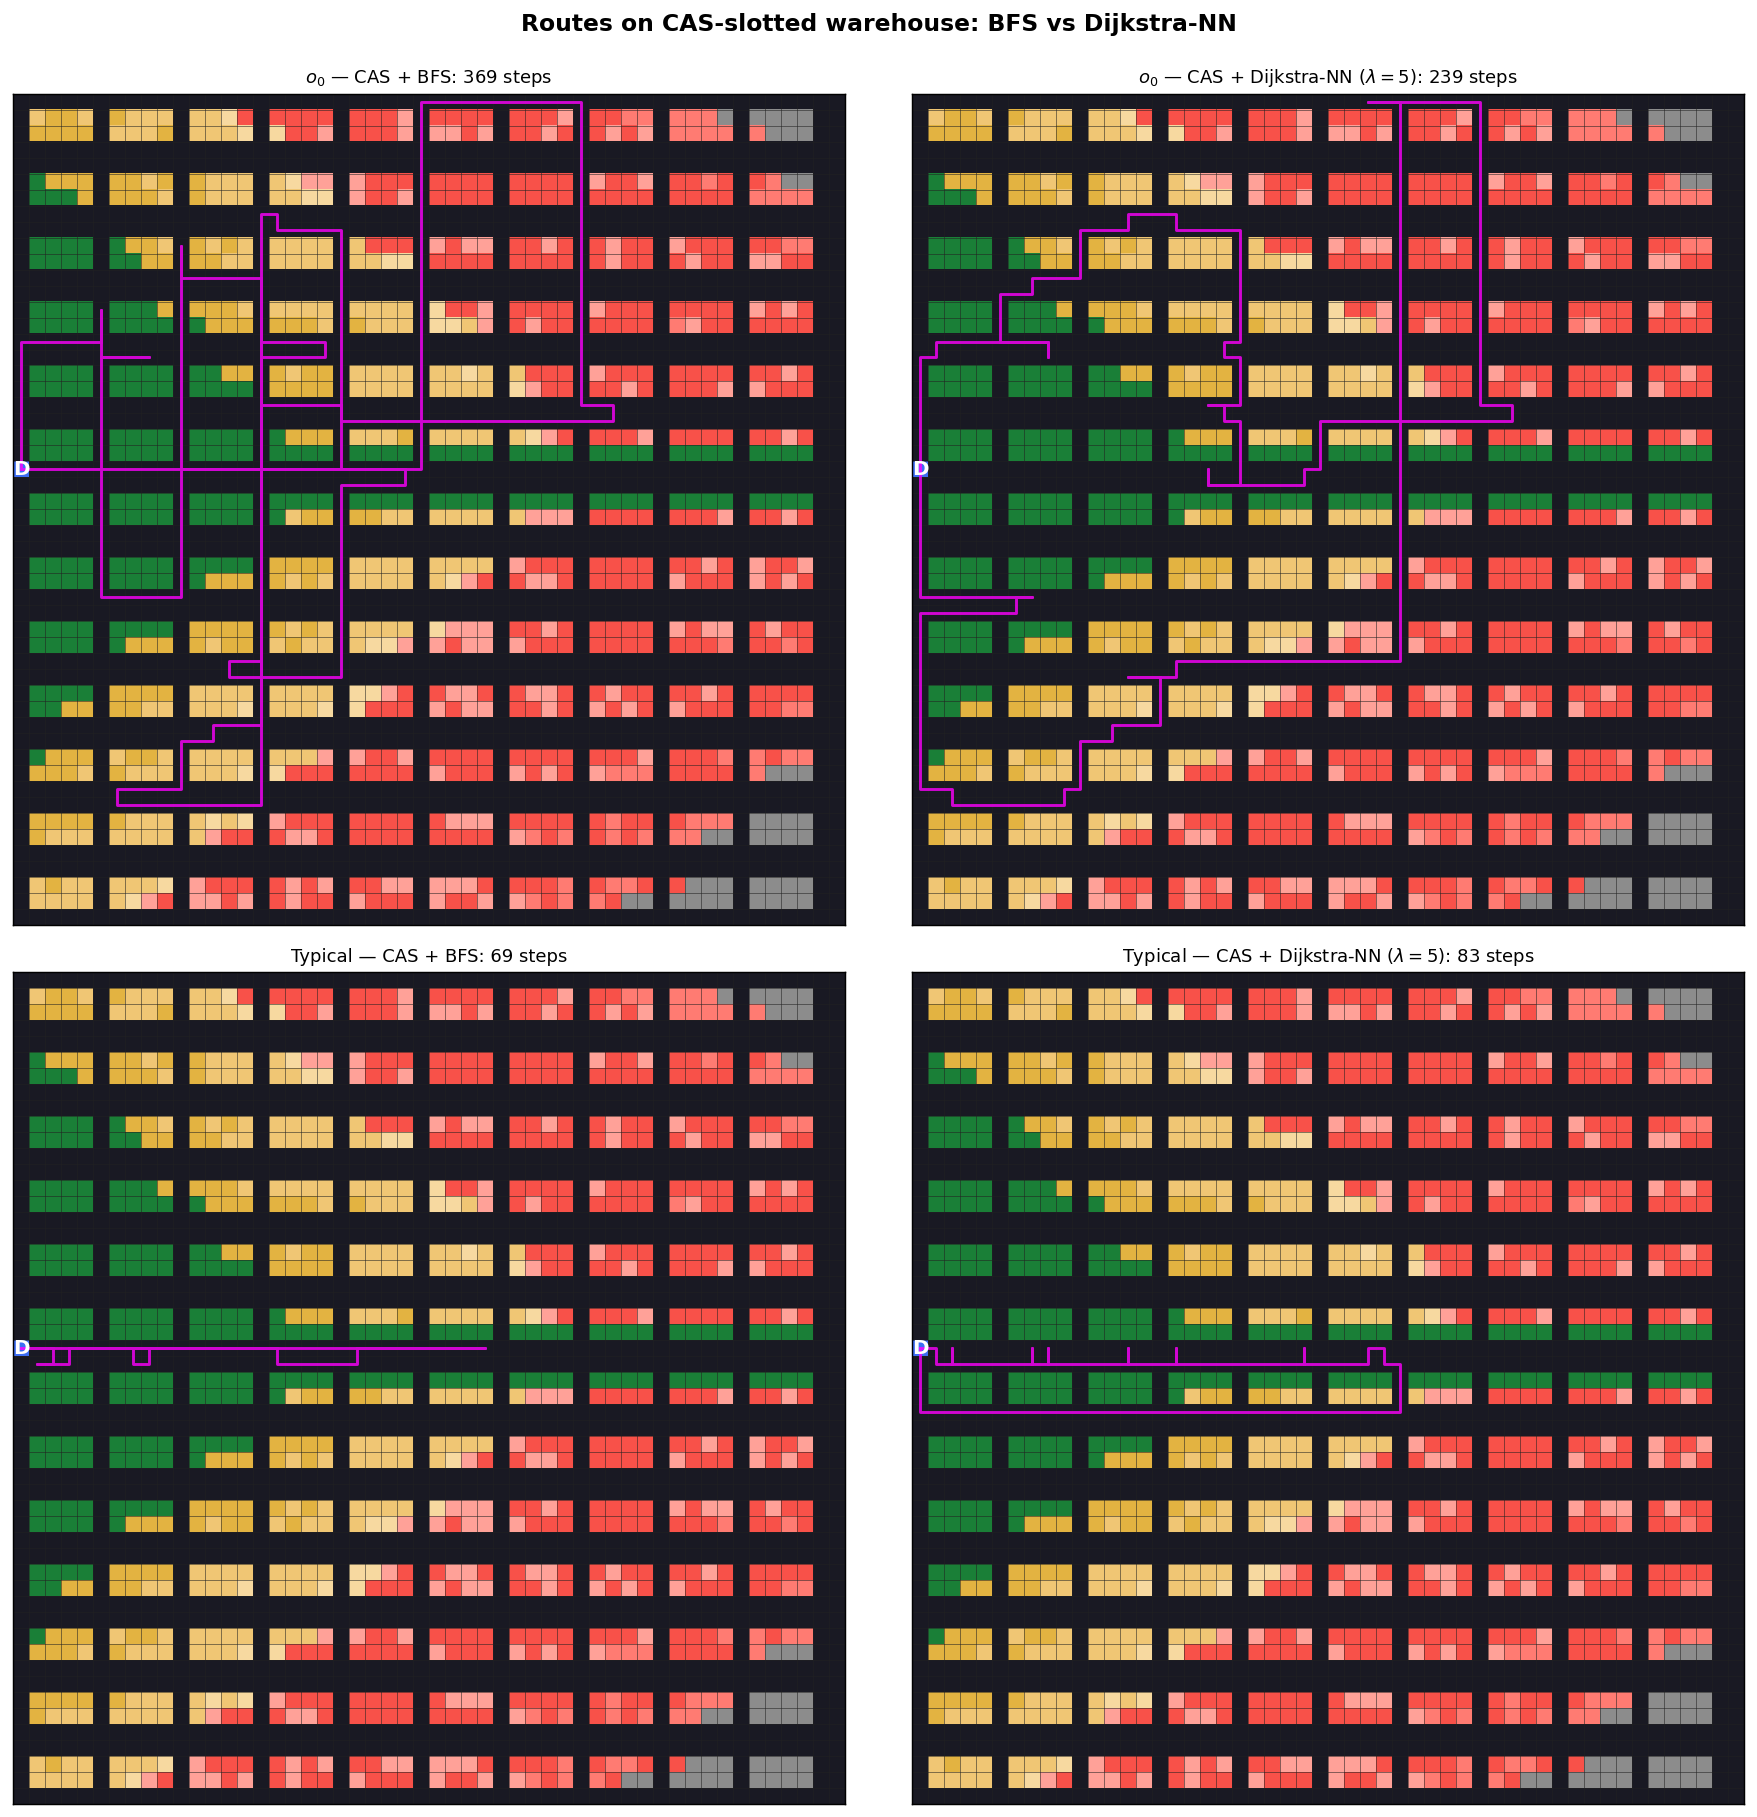
\includegraphics[width=\textwidth]{fig_config_c_routes.png}
  \caption{Routes on the CAS-slotted warehouse (specialised
    Config~C alternative).
    Rows: order $o_0$ (random) above; typical order below.
    Columns: BFS routing (left); Dijkstra-NN $\lambda = 5$ (right).
    Magenta = picking path; D = door.
    Dijkstra-NN shortens both routes; on the typical order the
    improvement is small (already short) but on $o_0$ it reroutes the
    detour through the cooler central corridor.}
  \label{fig:config_c_routes}
\end{figure}

\paragraph{Heat-map comparison: Baseline vs CAS vs AB under Dijkstra-NN.}
Figure~\ref{fig:three_way_heatmap} compares the traffic heat maps of
the three slottings (Baseline ABC$\times$XYZ, CAS, and Aisle-Balanced)
under the same Dijkstra-NN routing at $\lambda = 5$.
The three maps look visually similar at first glance: the
congestion-aware router actively spreads traffic across the warehouse
in all three layouts, and the dominant hot band sits along the door
axis (row $23$) in every case.
The differences appear in the peak visit counts and in the secondary
bands.
The Baseline (left) has the highest peak ($23\,712$ visits) with a
clearly concentrated hot stripe near the door; CAS (middle) has a
slightly lower peak ($23\,540$) but the hot band extends further
into the warehouse along the central corridor; and Aisle-Balanced
(right) has the lowest peak ($22\,921$, $-3.3\%$ versus Baseline)
with the most uniform spread of secondary bands across rows
$18$--$29$.
This pattern matches the numerical results of
Table~\ref{tab:config_c_matrix}: AB gives the shortest typical and
mean routes (its layout balances near-door traffic across several
rows), CAS gives the lowest WPC on the typical order (its
longitudinal A-band suits the top-15 SKU sweep), and the Baseline
sits between them with the most concentrated bottleneck.

\begin{figure}[H]
  \centering
  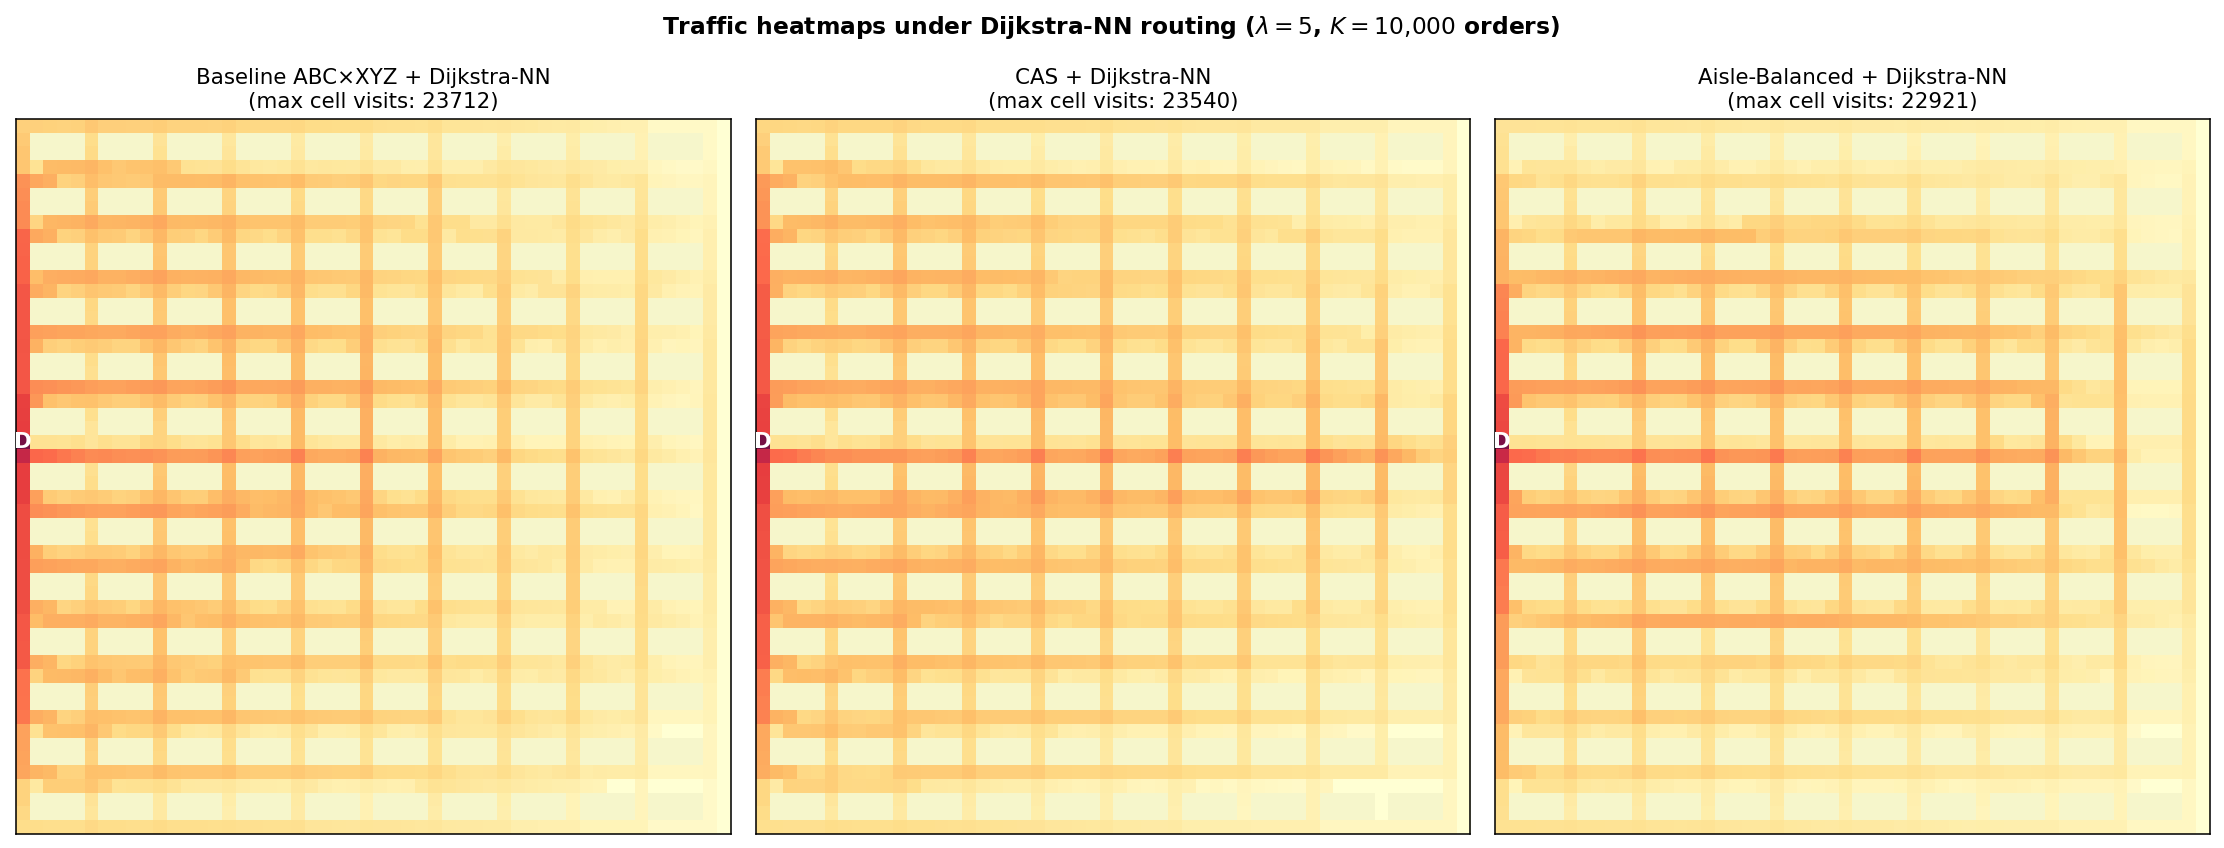
\includegraphics[width=\textwidth]{fig_three_way_heatmap.png}
  \caption{Traffic heat maps under Dijkstra-NN routing
    ($\lambda = 5$, $K = 10\,000$ orders).
    Left: Baseline ABC$\times$XYZ slotting. Middle: CAS slotting.
    Right: Aisle-Balanced slotting. All three panels use the same
    routing algorithm and order set, so any differences come purely
    from slotting. Shared YlOrRd colour scale with PowerNorm
    ($\gamma = 0.4$).}
  \label{fig:three_way_heatmap}
\end{figure}

\subsection{Discussion}

The Config~C experiment delivers three findings that revise the
single-axis conclusions of Sections~9.3 and 9.4.

\emph{Routing and slotting compose multiplicatively.}
The expected WPC under Config~C if the effects were merely additive
would be around $-117\%$ (Config~A's $-69.9\%$ plus Config B-CAS's
$-47.1\%$ on a Baseline of $55.86$~WPC --- the additive model produces
a number below zero, which is incoherent).
The actual $-83.6\%$ figure is consistent with the multiplicative model
in which slotting reduces the average $c_e$ a route encounters and
routing further reduces the route's contact with the remaining hot
edges; each axis works on the residual after the other has acted.

\emph{The recommended configuration changes from AB (with BFS) to
AB + Dijkstra-NN.}
In Section~9.3.6, Aisle-Balanced was recommended as the best
single-axis intervention; that recommendation now upgrades to
AB + Dijkstra-NN, which improves every metric over plain AB while
introducing no new computational cost beyond what Config~A already
required.
The hard-constraint criterion (route length) is satisfied on both
order types, and the soft objective (WPC) is reduced by a further
$50\%$--$55\%$ over plain AB.

\emph{CAS + Dijkstra-NN is the typical-order optimum but not the
recommended default.}
For installations where the demand mix is highly concentrated and
stable, CAS + CA provides the maximum reachable typical-order
performance.
For installations where mix robustness matters --- the more common
operational case --- AB + CA dominates.
This is a real trade-off rather than a strict preference, and the
choice is operator-dependent.

The original $2\times2$ design therefore yields a refined recommendation:
\begin{itemize}
  \item \textbf{Best routing only (no physical reshuffle):} Config~A
        (Dijkstra-NN on ABC$\times$XYZ slotting). $-77.4\%$ mean WPC,
        $-34.7\%$ mean steps, no warehouse changes required.
  \item \textbf{Best general-purpose (recommended):} Config~C with
        Aisle-Balanced slotting. Best mean batch route length ($211.2$~steps),
        best typical steps ($63$), competitive WPC on both order types.
  \item \textbf{Maximum typical-WPC reduction:}
        Config~C with CAS slotting. $-83.6\%$ typical WPC,
        WPC~$9.15$; fragile to demand shifts
        (typical-route steps $83$ vs.\ AB~+~CA's $63$).
\end{itemize}

%======================================================================
\section{Conclusion}
%======================================================================

This study investigated whether combining congestion-aware routing with
heat-map-informed slotting can reduce both route length and aisle
congestion in a small-to-medium single-depot warehouse. The proposed
$2 \times 2$ experimental design separated the slotting axis from the
routing axis and measured the contribution of each axis on its own
as well as their combined effect. Within Config~C, seven concrete
slotting strategies (Baseline, DWC, HZR, TAPS, Aisle-Balanced, AAHMS,
and CAS) were evaluated under Dijkstra-NN routing, and the most balanced
one was selected as the practical recommendation.

\paragraph{Main findings.}
\begin{itemize}
  \item Routing alone (Config~A, Dijkstra-NN at $\lambda = 5$) reduced
        mean route length from $339.8$ to $221.9$ steps ($-34.7\%$) and
        mean WPC from $108.5$ to $24.57$ ($-77.4\%$) without any
        physical reshuffle of items.
  \item Slotting alone (Config~B): among six slotting variants tested
        with BFS routing, Aisle-Balanced offered the best balance on
        the typical order ($107$ steps, WPC $46.25$), and CAS gave the
        strongest typical-order numbers ($69$ steps, WPC $29.56$) at
        the cost of weaker performance on the random order $o_0$.
  \item Combining both axes (Config~C) gave the largest overall gains.
        With Aisle-Balanced slotting, mean batch route length was
        $211.2$ steps and typical-order WPC was $10.62$.
        With CAS slotting, typical-order WPC reached $9.15$
        ($-83.6\%$ vs.\ Baseline).
  \item The two axes appear to compose closer to multiplicatively than
        additively: the observed Config~C reduction ($-83.6\%$) is
        within $0.5$ percentage points of the multiplicative prediction
        ($-84.1\%$).
\end{itemize}

\paragraph{Recommendation.}
For the present warehouse, Aisle-Balanced slotting combined with
Dijkstra-NN routing ($\lambda = 5$) is recommended as the best
general-purpose configuration: it has the shortest typical route
($63$~steps), the best mean batch route length ($211.2$~steps), and
competitive WPC on both order types. CAS combined with Dijkstra-NN is
retained as a specialised option for installations whose demand mix
is stable and strongly concentrated.

\paragraph{Limitations.}
The results were obtained from a single synthetic warehouse layout
($52 \times 52$ grid, $1\,000$ SKUs) and a single demand distribution
($10\,000$ orders generated from the Kaggle dataset).
The model assumes a single picker, unit shelf capacity, and a fixed
edge-congestion field, so multi-picker dynamic interactions are not
captured. The reported numerical values therefore describe relative
behaviour in the tested setting and should not be read as absolute
targets for real warehouses.

%======================================================================
\section{Future Work}
%======================================================================

Five directions seem most useful for follow-up research.

\paragraph{(i)~Validation on more realistic layouts.}
The present results were obtained on a single $52 \times 52$ grid with
uniform aisle width and no cross-aisles. Repeating the $7 \times 2$
matrix on layouts with cross-aisles, heterogeneous aisle widths, and
one-way picking lanes would test whether the AB/CAS trade-off holds in
more realistic geometries.

\paragraph{(ii)~Multi-picker simulation with dynamic congestion.}
The current model uses a static congestion field $c_e$ computed once
from the baseline simulation. Extending the model to a multi-picker
simulation, in which congestion is updated as pickers move, would
allow the $L_{95}$ metric to capture real-time interactions and
queueing effects between pickers.

\paragraph{(iii)~Held-out evaluation over multiple order samples.}
All experiments use a single fixed seed ($42$) and the same $10\,000$
orders both for heat-map construction and for evaluation, as justified
in Section~5.5. A more elaborate protocol --- for example, $k$-fold
averaging over multiple independent order samples generated under
different seeds --- would measure the variance of the reported metrics
and confirm that the recommended configurations remain best across
samples.

\paragraph{(iv)~Other routing algorithms.}
This work compared two routing algorithms: BFS (Baseline) and
Dijkstra-NN (Config~A and Config~C). A natural next step is to compare
with other shortest-path algorithms, such as A$^{*}$ with a
door-distance heuristic. A$^{*}$ should give the same paths as
Dijkstra under an admissible heuristic but with lower runtime cost.
The present study used Dijkstra-NN because it was the simplest variant
consistent with the $1 + \lambda c_e$ cost; a wider comparison would
test whether faster heuristic search changes the speed--quality
trade-off in practice.

\paragraph{(v)~Additional evaluation metrics.}
The current evaluation uses three metrics: mean route length, $L_{95}$,
and WPC. A useful extension is the \emph{Congestion Relief Ratio}
(CRR), defined as the share of baseline-routing corridor cells that
the alternative strategy avoids:
\[
  \mathrm{CRR} = \frac{|\{\text{cells in BFS path}\} \setminus \{\text{cells in CA path}\}|}
                       {|\{\text{cells in BFS path}\}|}.
\]
CRR gives a direct spatial measure of how much of the originally hot
area is actually avoided. Values close to~$1$ mean that the
alternative route bypasses almost all of the previously congested
segments; values close to~$0$ mean that the two routes share most of
the same bottlenecks. CRR was not used in the main analysis because
WPC already captures the same effect in weighted form, but reporting
CRR alongside WPC would help distinguish ``slight congestion
reduction along the same path'' from ``actual rerouting around the
hot zone'', which is informative in spatial discussions.

\newpage
%======================================================================
\begin{thebibliography}{9}
\addcontentsline{toc}{section}{Bibliography}

\bibitem{ref1}
Trubchenko, T.\,G., Kiseleva, E.\,S., Loshchilova, M.\,A., Dreval, A.\,N., Ryzhakina, T.\,G., \& Shaftelskaya, N.\,V.
Application of ABC and XYZ analysis to inventory optimisation at a commercial enterprise.
\textit{SHS Web of Conferences}, 80, 01007, 2020.
\url{https://doi.org/10.1051/shsconf/20208001007}

\bibitem{ref2}
Pekar\v{c}\'{i}kov\'{a}, M., Kliment, M., Kronov\'{a}, J., Trebu\v{n}a, P., \& Hovana, A.
Simulation-based optimisation of material supply in automotive production using RTLS data.
\textit{Applied Sciences}, 15(16), 9102, 2025.

\bibitem{ref3}
Kofler, M., Beham, A., Wagner, S., \& Affenzeller, M.
Affinity-based slotting in warehouses with dynamic order patterns.
In: Klempous, R., Nikodem, J., Jacak, W., \& Chaczko, Z. (Eds.),
\textit{Advanced Methods and Applications in Computational Intelligence}.
Topics in Intelligent Engineering and Informatics, vol.~6.
Springer, Heidelberg, 2014.
\url{https://doi.org/10.1007/978-3-319-01436-4_7}

\bibitem{ref4}
Winkelhaus, S., \& Grosse, E.\,H.
Logistics 4.0: a systematic review towards a new logistics system.
\textit{International Journal of Production Research}, 58(1), 18--43, 2020.
\url{https://doi.org/10.1080/00207543.2019.1612964}

\bibitem{ref9}
M\"{u}ller, J.\,M.
The impact of data-driven technologies on supply chain design.
In \textit{Proceedings of the 43rd International Conference on Information Systems
(ICIS 2022), Special Interest Group on Big Data}, AIS Electronic Library, Copenhagen, 2022.

\bibitem{ref10}
Stroumpoulis, A., \& Kopanaki, E.
Theoretical perspectives on sustainable supply chain management and digital
transformation: a literature review and a conceptual framework.
\textit{Sustainability}, 14(8), 4862, 2022.
\url{https://doi.org/10.3390/su14084862}

\bibitem{ref5}
Hagle, C. Maximizing warehouse productivity with heat maps.
\textit{Pallets of Wisdom} (blog), LIDD Consultants, 2023.
Available at: \url{https://lidd.com/warehouse-productivity-heat-maps/}
(date accessed: 24 May 2026).

\bibitem{ref6}
Kabir, S. ABC-XYZ Inventory Classification Dataset.
\textit{Kaggle}, 2024.
Monthly demand data and sales values for inventory segmentation analysis.
Available at: \url{https://www.kaggle.com/datasets/shahriarkabir/abc-xyz-inventory-classification-dataset}
(date accessed: 24 May 2026).

\bibitem{ref7}
Casella, G., Volpi, A., Montanari, R., Tebaldi, L., \& Bottani, E.
Trends in order picking: a 2007--2022 literature review.
\textit{Production \& Manufacturing Research}, 11(1), 2191115, 2023.
\url{https://doi.org/10.1080/21693277.2023.2191115}

\bibitem{ref8}
GEODIS. Warehouse optimisation: slotting \& wave pick improvement.
\textit{GEODIS Blog}, GEODIS Group, 2023.
Available at: \url{https://geodis.com/us-en/blog/warehouse-optimisation-slotting-wave-pick-improvement}
(date accessed: 24 May 2026).

\bibitem{ref_ratliff}
Ratliff, H.\,D. \& Rosenthal, A.\,S.
Order-picking in a rectangular warehouse: a solvable case of the travelling salesman
problem.
\textit{Operations Research}, 31(3), 507--521, 1983.

\bibitem{ref_petersen}
Petersen, C.\,G.
An evaluation of order picking routeing policies.
\textit{International Journal of Operations \& Production Management}, 17(11),
1098--1111, 1997.

\end{thebibliography}

\end{document}
